\documentclass[usenatbib,fleqn]{mn2e}

\makeatletter
\newlength{\abovecaptionskip}%
\setlength{\abovecaptionskip}{10\p@}
\makeatother
\usepackage{threeparttable}


\usepackage{amsmath,amssymb}
\usepackage{mathrsfs}
\usepackage{graphicx}
\usepackage{epstopdf}
\usepackage{hyperref}
\epstopdfsetup{outdir=./figures/}
\graphicspath{{./figures/}}
\usepackage{url}
\usepackage{aas_macros}
\usepackage{astro}
\usepackage{deluxetable}
% \usepackage{natbib}

% \renewcommand{\l}{\left}
% \renewcommand{\r}{\right}

\newcommand{\Mdot}{\dot{M}}
\newcommand{\eddr}{\dot{M}/\dot{M}_{\rm Edd}}
\newcommand{\MdotEdd}{\dot{M}_{\rm Edd}}
\newcommand{\Mdotb}{\dot{M}_{\rm bondi}}

\newcommand\lsim{\mathrel{\rlap{\lower4pt\hbox{\hskip1pt$\sim$}}
    \raise1pt\hbox{$<$}}}
\newcommand\gsim{\mathrel{\rlap{\lower4pt\hbox{\hskip1pt$\sim$}}
    \raise1pt\hbox{$>$}}}
\newcommand{\rs}{r_s}
\newcommand{\rb}{r_b}
\newcommand{\rcirc}{r_{\rm circ}}
\newcommand{\rss}{r_{\rm ss}}
\newcommand{\lrs}{\l_{\rs}}
\newcommand{\lambdars}{\lambda_{\rs}}
\newcommand{\vw}{\tilde{v}_{w}}

\newcommand{\dxdy}[2]{\frac{d #1}{d #2} }
\newcommand{\ddr}[1]{\dxdy{#1}{r}}
\newcommand{\drhodt}{\dxdy{\rho}{t}}
\newcommand{\dpdr}{\dxdy{p}{r}}
\newcommand{\dvdr}{\dxdy{v}{r}}
\newcommand{\dsdr}{\dxdy{s}{r}}
\newcommand{\dphidr}{\dxdy{\Phi}{r}}

\newcommand{\ke}{\frac{v^2}{2}}
\newcommand{\kew}{\frac{\tilde{v}_{w}^2}{2}}

\newcommand{\gammaf}{\frac{\gamma}{\gamma-1}}
\newcommand{\gammafi}{\frac{\gamma-1}{\gamma}}
\newcommand{\cs}{\frac{p}{\rho}}
\newcommand{\Q}{q (\ke+\kew-\gammaf \cs)}

\newcommand{\kb}{k_{\rm b}}
\renewcommand{\mp}{m_{\rm p}}
\newcommand{\pc}{\rm pc}

\newcommand{\Menc}{M_{\rm enc}}
\newcommand{\rhostar}{\rho_*}
\newcommand{\Mstar}{M_{\star}}
\newcommand{\Mseight}{M_{\star,8}}
\newcommand{\Mbh}[1][]{M_{\bullet#1}}
\newcommand{\Mbheight}{M_{\bullet,8}}
\newcommand{\MbheightExp}{\frac{\Mbh}{10^8 \Msun}}

\newcommand{\phirs}{\frac{G \Menc}{\rs}}
\newcommand{\soi}{\rm soi}
\newcommand{\rsoi}{r_{\soi}}
\newcommand{\rIa}{r_{\rm Ia}}
\newcommand{\EIa}{E_{\rm Ia}}
\newcommand{\RateIa}{R_{\rm Ia}}
\newcommand{\sigsoi}{\sigma_{\soi}}

\newcommand{\vwO}{v_{w}}
\newcommand{\kewO}{\frac{\vwO^2}{2}}
\newcommand{\x}{\frac{r_s}{\rsoi}}
\newcommand{\vwNorm}{\frac{\vwO}{\sigsoi}}
\newcommand{\vwOFH}{v_{500}}
\newcommand{\vwOFHexp}{\frac{\vwO}{500 \, {\rm km/s}}}

\newcommand{\pyear}{{\rm yr}^{-1}}
\newcommand{\tage}{t_{\star}}
\renewcommand{\th}{t_h}
\newcommand{\tcool}{t_{\rm cool}}
\newcommand{\tff}{t_{\rm ff}}

\newcommand{\densSlope}{\nu}

\topmargin -1 cm

\author[Generozov, Stone, \& Metzger]{Aleksey Generozov$\thanks{E-mail: ag@astro.columbia.edu}$, Nicholas Stone, Brian~D.~Metzger\\
  Columbia Astrophysics Laboratory, Columbia University, 550 West 120th
  Street, New York, NY 10027}


\begin{document}
\title{Circumnuclear Media and Accretion Rates of Quiescent Supermassive Black Holes}
\maketitle

\begin{abstract}
  We calculate steady-state, one-dimensional hydrodynamic profiles of
  hot gas in the nuclei of nominally quiescent galaxies for a range of
  central black hole mass $M_{\bullet}$, parameterized gas heating
  rate, and observationally-motivated stellar density profiles.  Mass
  is supplied to the circumnuclear medium by stellar winds, while gas
  is heated primarily by stellar winds, supernovae, and black hole
  feedback.  Analytic estimates are provided for the stagnation radius
  (where the radial velocity of the gas passes through zero) and the
  black hole mass accretion rate, $\dot{M}$, as a function of black
  hole mass and the gas heating efficiency, the latter of which is
  related to the star-formation history.  We assess the conditions
  under which radiative instabilities develop, separately in the case
  of a single burst of star formation and in the case of the average
  star formation history of galaxies hosting a given black hole
  mass. The measured nuclear X-ray luminosities, $L_{X}$, of a sample
  of quiescent black holes are combined with our results for $\dot{M}$
  to conclude that early-type quiescent black holes in the local
  universe are consistent with accreting in a locally thermally-stable
  state (on scales of the sphere of influence), possibly between
  cycles of thermal instability on larger galactic scales.  The
  maximum accretion rate of a thermally-stable flow is too low to
  explain the short growth times of low mass black holes in the local
  universe.  The latter must instead result from gas being fed in from
  large radii, either due to galaxy mergers associated with
  hierarchical growth or thermal instabilities on larger, galactic
  scales.  Our results have implications for attempts to constrain the
  occupation fraction of SMBHs in low mass galaxies using the mean
  $L_{\rm X}-M_{\bullet}$ correlation, as well as to the diversity of
  circumnuclear media densities encountered by relativistic jets from
  tidal disruption events.
\end{abstract}

\begin{keywords}
  black hole physics --  galaxies: active
\end{keywords}


\section{Introduction}
\label{sec:introduction}

Supermassive black holes (SMBHs) lurk in the centers of most, if not
all nearby galaxies (see reviews by,
e.g. \citealt{KormendyRichstone:1995a};
\citealt{FerrareseFord:2005a}). However, only a few percent of these
manifest themselves as luminous Active Galactic Nuclei (AGN).  Nearly
quiescent SMBHs, such as those hosting low luminosity AGN, constitute
a silent majority (e.g.~\citealt{Ho:2009a}).

Understanding why most SMBHs appear to be inactive requires
characterizing their gaseous environments.  Gas near the sphere of
influence of the SMBH, hereafter the `circumnuclear medium' (CNM),
controls the mass accretion rate, $\dot{M}$.  The accretion rate in
turn sets the luminosity of the black hole and the impact of this
energy and momentum output on larger physical scales (`feedback').
The presence of dense gas in the nuclear region may also lead to runaway
cooling, resulting in bursty episodes of star formation and AGN
activity (e.g.~\citealt{Ciotti&Ostriker07}; \citealt{Ciotti+10}).

Knowledge of how $\dot{M}$ depends on the SMBH mass, $\Mbh$, and other
properties of the galactic nucleus informs key questions related to
the co-evolution of SMBHs and their host galaxies with cosmic time
(e.g.~\citealt{Kormendy&Ho13}; \citealt{HeckmanBest:2014a}).  SMBH growth
in the low redshift universe is dominated by low mass black holes,
$M_{\bullet} \lesssim 10^{8}M_{\odot}$ (e.g.~\citealt{Heckman+04}), a
fact which is often attributed to the general trend of `cosmic
down-sizing' resulting from hierarchical structure growth (e.g,
\citealt{Gallo+08}).  However, the physical processes involved in
growing low mass blacks may be distinct from those operating at higher
SMBH masses and accretion rates in quasars.  A key open question is
whether SMBHs grow primarily by accreting gas fed in directly from
galactic or extra-galactic scales, or whether significant growth
results also from internal, secular processes such as local stellar
mass loss in the nuclear region.

A better understanding of what mechanisms regulate accretion onto
quiescent SMBHs would have implications for a variety of observations,
such as constraints on the occupation fraction of SMBHs in low mass
galaxies.  \citet{Miller+15} use the average relationship between the
nuclear X-ray luminosities, $L_{X}$, of a sample of elliptical
galaxies and their associated SMBH masses to infer tentative evidence for a
SMBH occupation fraction less than unity in galaxies with stellar
masses $M_{\star} \lesssim 10^{10}M_{\odot}$ ($M_{\bullet} \lesssim
10^{7}M_{\odot}$).  This method relies on extrapolating a power-law
fit of the $L_X-\Mbh$ distribution to low values of $L_{\rm X}$ below
the detection threshold, a potentially problematic assumption if
different physical processes control the accretion rates onto the
lowest mass SMBHs.

%The conclusions of
%\citet{Miller+15} are thus sensitive to possible changes in
%the $L_X$-$\Mbh$ relationship at small $\Mbh$.
% AG: In our model we obtain a steeper relationship, but we have difficulty matching the observed relationship above the detection threshold

The gas density in galactic nuclei also influences the emission from
stellar tidal disruption events (TDEs), such as the high energy
transient {\it Swift} J1644+57 (\citealt{Levan+11};
\citealt{Bloom+11}, \citealt{Burrows+11}; \citealt{Zauderer+11}).
This transient event was powered by an impulsive relativistic jet,
which produced synchrotron radio emission as the jet material was
decelerated by shock interaction with the CNM of the previously
quiescent SMBH (\citealt{Giannios&Metzger11}; \citealt{Zauderer+11}).
Detailed modeling of J1644+57 showed that the CNM density was much
lower than that measured surrounding Sgr A$^{\star}$
(\citealt{Metzger+12}; \citealt{BergerZauderer+:2012a}).  However, a TDE jet
injected into a denser CNM would be decelerated more rapidly,
producing substantially different radio emission than in J1644+57.
Variations in the properties of the CNM could help explain why most
TDEs appear to be radio quiet (e.g.~\citealt{Bower+13};
\citealt{VanVelzen+13}).

Gas comprising the CNM can in principle originate from several
sources: (1) wind mass loss from predominantly evolved stars; (2)
stellar binary collisions; and (3) unbound debris from a recent TDE.
Stellar wind mass loss is probably the dominant source insofar as
collisions are relevant only in extremely dense stellar environments
for very young stellar populations (\citealt{Rubin&Loeb11}), while
\citet{MacLeod+13} find that TDEs contribute subdominantly to the
time-averaged accretion rate of quiescent SMBHs.

\citet{Ho:2009a} determines the SMBH accretion rates in a sample of
early-type galaxies using X-ray observations to determine the
Bondi accretion rate and based on estimates for the mass loss rate of
evolved stars.  Both methods lead to the conclusion that the available
gas reservoir is more than sufficient to power the observed
low-luminosity AGN, assuming the standard $\sim$ 10 per cent radiative
efficiency for thin disk accretion.  Much
evidence now suggest that low-luminosity AGN result from accretion
proceeding in a radiatively inefficient mode
(\citealt{Yuan&Narayan14}), due either to the advection of
gravitationally-released energy across the SMBH horizon
(e.g.~\citealt{Narayan&Yi95}) or due to the low efficiency with which the inflowing gas ultimately reaching the viscinity of the SMBH
(e.g.~\citealt{Blandford&Begelman99}; \citealt{Li+13}).

%In fact, the temperature profile is assumed to be flat inside of the
%Bondi radius.  In reality, the cusp in the velocity dispersion near
%the SMBH, should cause a cusp in the gas temperature profile (assuming
%the kinetic energy of stellar winds is efficiently thermalized in
%shocks).
%% AG-give sense of scale.

Another approach to determine the SMBH accretion rate, which we adopt
in this paper, is to directly calculate the density, velocity and
temperature profiles of the CNM using a physically motivated
hydrodynamic model.  Mass is injected to the nuclear environment via
stellar winds, while energy input results from several sources
including stellar winds, supernovae, and AGN feedback
(\citealt{Quataert:2004a,De-ColleGuillochon+:2012a,ShcherbakovWong+:2014a}).
Unlike previous works, which focused primarily on modeling individual galaxies, here
we systematically analyze the CNM properties across a range of galaxy properties, including different SMBH masses, stellar density profiles, and
star formation histories (\citealt{WangMerritt:2004a}).

Past studies, employing multi-dimensional numerical hydrodynamics and
including variety of (parameterized) physical effects, have focused on
massive elliptical galaxies (e.g.~\citealt{Ciotti&Ostriker07};
\citealt{Ciotti+10}).  A key finding of these works is the periodic
development of cooling instabilities on galactic scales, which
temporarily increase the gas accretion rate towards the nucleus until
feedback becomes effective to shut off the flow and halt
SMBH growth.  Here we instead focus on time-independent models,
neglecting radiative cooling.  This approach allows us to
systematically explore the relevant parameter space and to derive
simple analytic expressions that prove useful in exploring whether
cooling instabilties manifest across the expected range of galaxy
properties, or whether other (non-AGN) forms of feedback can result in
steady accretion.  Even if cooling instabilties develop on galactic
scales over longer $\sim$ Gyr timescales, a state of
quasi-steady accretion may exist between these inflow events on
smaller radial scales comparable to the sphere of influence.  We are
thus motivated to explore whether steady flow is achieved within the
nucleus under any circumstances, or whether the gas content is always
building towards instability.
%A chief goal of our analysis is to provide a framework for interpreting the properties of quiescent galactic nuclei given the comparatively well understood physics of stellar winds and supernova heating.

In the presence of strong heating, one-dimensional steady-state flow
is characterized by an inflow-outflow structure, with a critical
radius known as the``stagnation radius" $\rs$ where the radial
velocity passes through zero.  Mass loss from stars interior to the
stagnation radius is accreted, while that outside $\rs$ is unbound in
an outflow from the nucleus.  The stagnation radius, rather than the
Bondi radius, thus controls the SMBH accretion rate (although we will
show that $\rs$ can in many cases lie within a factor of few of the
nominal Bondi radius).  When heating is sufficiently weak, however, no stagnation radius may exist at all, i.e. the entire ISM of the galaxy is flowing towards the SMBH.  A key goal of this work is to
assess under what conditions a stagnation radius exists, as this
question is intimately tied to that of cooling instability.
% Furthermore, in some cases we find that no stagnation
% radius exists at all; this formally implies that the entire of ISM of
% the galaxy is feeding the SMBH, potentially resulting in much higher
% accretion rate than would be predicted by simple Bondi accretion. 


This paper is organized as followed.  In $\S\ref{sec:model}$ we
describe our model, including the sample of galaxies used in our
analysis ($\S\ref{sec:gal_model}$) and our numerical procedure for
calculating the steady-state hydrodynamic profile of the CNM
($\S\ref{sec:hydro}$).  In $\S\ref{sec:results}$ we describe some
analytic results, while in $\S\ref{sec:numerical}$ we describe our numerical results.  In $\S\ref{sec:discussion}$ we discuss the implications of our results, to topics including...   In $\S\ref{sec:conclusions}$ we summarize our conclusions.  Table \ref{table:definitions} provides the definitions of commonly used variables.  Appendices \ref{app:rs} and XXX provides useful analytic results, while Appendix \ref{app:windheat} describes our method for calculating stellar wind heating and mass input in greater detail.  


\begin{table*}
\begin{threeparttable}
%\centering
\begin{minipage}{18cm}
\caption{Definitions of commonly used variables}
\begin{tabular}{ll}
\hline
{Variable} & {Definition} \\
\hline
$M_{\bullet}$ & Black hole mass \\
$\tilde{v}_{w}$ & Total heating parameter, including minimum heating
rate from stellar and black hole velocity dispersion \\
$v_{w}$ & Total heating parameter, excluding heating rate from velocity dispersion \\
$r_{s}$ & Stagnation radius (where gas radial velocity goes to zero) \\
$r_{\rm soi}$ & radius of sphere of influence (eq.~[\ref{eq:rsoi}]) \\
$r_{\rm b}$ & outer break radius of stellar density profile \\ 
$r_{\rm Ia}$ & radius interior to which Ia SN are infrequent compared to the dynamical/inflow timescale (eq.~[\ref{eq:rIa}]) \\ 
$\rho_{\star}(r)$ & 3D radial stellar density profile \\
$\rho(r)$ & gas density of CNM \\
$M_{\star}(r)$ & total enclosed stellar mass inside radius $r$ \\
$M_{\rm enc}(r)$ & total encolsed mass inside radius $r$ (SMBH + stars) \\
$q(r)$ & mass source term due to stellar winds (eq.~[\ref{eq:q}]) \\
$\eta$ & parameter setting normalization of mass input from stellar winds (eq.~[\ref{eq:q}]) \\
$\tau_{\star}$ & age of stellar population, in case of a single burst of star formation \\
$\Gamma$ & power-law slope of radial stellar density profile interior to the break radius \\
$\sigma(r)$ & stellar velocity dispersion \\
$\dot{M}$ & mass accretion rate \\
$\dot{M}_{\rm Ia}$ & maximum mass accretion rate as limited by SN Ia blow-out (eq.~[\ref{eq:eddr_Ia}]) \\
$\dot{M}_{\rm C}$ & equilibrium accretion rate set by Compton heating (eq.~[\ref{eq:MdotC}]) \\
$\dot{M}_{\rm TI}$ & maximum accretion rate for thermally stable accretion (eq.~[\ref{eq:Mdotmax}]) \\
$\dot{q}_{\rm heat}/|\dot{q}_{\rm rad}|$ & ratio of external heating (stellar winds, SN Ia, MSPs) to radiative cooling (eq.~[\ref{eq:cooling2}]) \\
$t_{\rm h}$ & Hubble timescale \\
$\nu$ & gas density power-law slope at the stagnation radius (eq.~[\ref{eq:densSlope}]) \\
\hline
\label{table:definitions}  
\end{tabular}
\begin{tablenotes}
\item{$^{(a)}FILL IN$}
\end{tablenotes}
\end{minipage}
\end{threeparttable}

\end{table*}


\section{Model}
\label{sec:model}
\subsection{Galaxy models}
\label{sec:gal_model}
\citet{LauerFaber+:2007a} use Hubble Space Telescope WFPC2 imaging to
measure the radial surface brightness profiles for hundreds of nearby
early type galaxies. The measured brightness profile is generally
well-fit by a ``Nuker" law parameterization:
\begin{equation}
  I(\xi)=I_b 2^{(\beta-\Gamma)/\alpha} \xi^{-\Gamma} (1+\xi^\alpha)^{-(\beta-\Gamma)/\alpha}, \,\,\,\xi\equiv\frac{r}{r_b},
\end{equation}
i.e., a broken power law that transitions from an inner power law
slope, $\Gamma$, to an outer power law slope, $\beta > \Gamma$, at a
break radius, $\rb$.  Assuming the stellar population is spherically
symmetric, this corresponds to a stellar density $\rhostar \propto
r^{-1-\Gamma}$ for $r \ll \rb$ and $\rhostar\propto r^{-1-\beta}$ for
$r \gg \rb$.  To good approximation
\begin{align}
\rho_\star = 
\begin{cases}
\rho_\star|_{\rsoi} \left(r/\rsoi\right)^{-1-\Gamma} & r \leq r_b\\
\rho_\star|_{r_b} \left(r/r_b\right)^{-1-\beta} & r > r_b,
\label{eq:rhostar}
\end{cases}
\end{align}
where $\rho_\star|_{\rsoi}$ is the stellar density at the radius of the black hole sphere of influence (soi), 
\begin{equation}
\rsoi \simeq G \Mbh/\sigma^2 \approx 14 M_{\bullet,8}^{0.6}\,{\rm pc},
\label{eq:rsoi}
\end{equation}
where $M_{\bullet,8} \equiv M_{\bullet}/10^{8}M_{\odot}$ and the
second equality in (\ref{eq:rsoi}) employs the $\Mbh-\sigma$
relationship of \citet{McConnellMa+:2011a},
 \begin{align}
M_{\bullet} \simeq 2\times 10^{8}\left(\frac{\sigma}{200\,{\rm
      km\,s^{-1}}}\right)^{5.1}M_{\odot}.
\label{eq:Msigma}
\end{align}
Though of questionable validity for low mass black holes (e.g., \citealt{Greene&Ho07}), we adopt equation (\ref{eq:Msigma}) for lack of a better alternative.

A galaxy model is fully specified by four parameters: $\Mbh$,
$\Gamma$, $r_b$, and $\beta$.  We compute models for three different
black hole masses, $\Mbh = 10^6$, $10^7$, $10^8 \Msun$.  The
distribution of $\Gamma$ in the \citet{LauerFaber+:2007a} sample is
bimodal, with a concentration of ``core" galaxies with $\Gamma \lsim
0.3$ and a concentration of ``cusp" galaxies with $\Gamma \gsim 0.7$.
We bracket these possibilities by considering models with $\Gamma=0.8$
and $\Gamma=0.1$.  

We fix $\beta = 2$ (a typical value) because our results are generally
not sensitive to the properties of the gas flow on radial scales
$\gtrsim r_b$. The presence of the break radius $r_{b}$ is, however,
necessary to obtain a converged steady state for some regions of our
parameter space.  We consider solutions calculated for up to four
values of $\rb$: 50 pc, 100 pc, 200 pc, and 400 pc, motivated by the
range of break radii from the \citet{LauerFaber+:2007a}
sample.\footnote{For the core galaxies the break radius follows the
  scaling relationship $\rb\sim 106 \, (\Mbheight)^{0.39}$ pc, with
  scatter of approximately one dex.  Most the cusp galaxies have $\rb$
  between 100 and 1000 pc, without a clear trend with $\Mbh$.}  In
practice we calculate solutions for a range of $\rb$ only in cases
when its precise value is expected to have a significant affect on the
solution, in particular for high SMBH masses and low heating rates,
for which the stagnation radius approaches large radii.


\subsection{Hydrodynamic Equations}
\label{sec:hydro}

Following \citet{Quataert:2004a} (see also \citealt{HolzerAxford:1970a,De-ColleGuillochon+:2012a,ShcherbakovWong+:2014a}), we calculate the density $\rho$, temperature $T$, and radial velocity $v$ of the CNM for each galaxy model by solving the equations of one-dimensional, time-dependent hydrodynamics,
\begin{align}
  &\drhodt+\frac{1}{r^2}\frac{\partial}{\partial r}\left(\rho r^2 v\right)=q \label{eq:drhodt}\\
  &\rho \left(\frac{\partial v}{\partial t} + v\frac{\partial
      v}{\partial r}\right) =-\frac{\partial p}{\partial r}- \rho\frac{GM_{\rm enc}}{r^{2}} -q v \label{eq:dvdt}\\
  &\rho T\left(\frac{\partial s}{\partial t} + v\frac{\partial
      s}{\partial r}\right)=q\left[\ke+\kew-\gammaf \cs \right] 
, 
\label{eq:dsdt}
\end{align}
where $p$ and $s$ are the pressure and specific entropy, respectively, and $M_{\rm enc} = M_{\star}(r) + \Mbh$ is the
enclosed mass.  We adopt an ideal gas equation of state with $p = \rho kT/\mu m_p$ with $\mu = 0.62$  and $\gamma = 5/3$. 

The source term in equation (\ref{eq:drhodt}),
\begin{align}
  q=\frac{\eta \rhostar}{\th},
\label{eq:q}
\end{align}
represents mass input from stellar winds, which we parameterize in
terms of the fraction $\eta$ of the stellar density $\rhostar$ being
recycled into gas on the Hubble time $\th = 1.4 \times 10^{10}$ yr.
To good approximation $\eta\simeq 0.02 (\tau_{\star}/t_h)^{-1.3}$ at
time $\tau_{\star}$ following an impulsive star burst (e.g.,
\citealt{Ciotti+91})\footnote{\citet{Ciotti+91} give the mass return
  rate from evolved stars as a function of B-band luminosity instead
  of volumetrically, but our expressions are equivalent.}, although
$\eta$ is significantly higher for continuous star formation histories
(bottom panel of Fig.~\ref{fig:vwSources}).

Source terms $\propto q$ also appear in the momentum and entropy
equations (eqs.~[\ref{eq:dvdt}] and [\ref{eq:dsdt}]) because the isotropic injection of mass represents, in the SMBH rest frame, a source of momentum
and energy relative to the mean flow.  Physically, these result from
the mismatch between the properties of virialized gas injected locally
by stellar winds and the mean properties of the background flow.  The
term $\propto -q c_{s}^{2}$ is important because it acts to potentially stabilize the flow to runaway cooling ($\S\ref{sec:instability}$).

The term $\propto \vw^2 = \sigma(r)^2+v_{w}^2$ in the entropy equation
accounts for external heating sources (e.g.,
\citealt{ShcherbakovWong+:2014a}).  The first term approximates the
minimum amount of shock heating from stellar winds due to the random
movement of stars with respect to one another at the characteristic
velocity of $\sigma \approx \sqrt{GM_{\rm enc}/r}$.  This heating is
present even in old stellar populations for which mass and energy
injection are dominated by AGB winds with low velocities $\ll \sigma$.
The second term, $v_{w}^{2}$, parameterizes all additional sources of
heating, including faster main sequence or Wolf-Rayet stellar winds,
spin-down energy from millisecond pulsars, supernovae, AGN feedback,
etc.  As will be discussed in $\S\ref{sec:heating}$, the value of
$v_{w}$ will in general depend on the SMBH mass and the age of the
stellar population.  We further assume that $v_w$ is constant with
radius, i.e. that the volumetric heating rate is proportional to the
local stellar density.

To isolate the physics of interest, our baseline calculations neglects three potentially important effects: heat conduction, radiative cooling, and rotation.  Electron heat conduction results in an an additional term on the right hand side of the entropy equation of the form:  
\begin{equation}
\dot{q}_{\rm cond} = \nabla\cdot(\kappa \nabla T),
\label{eq:qdotcond}
 \end{equation}
where $\kappa_{\rm
  eff}=\kappa_{\rm spitz}/(1+\psi)$ (\citealt{DaltonBalbus:1993a}) is
the conducitivity and $\kappa_{\rm spitz} = \kappa_0 T^{5/2}$ is the
classical \citet{Spitzer62} value ($\kappa_0\simeq 2\times 10^{-6}$ in
cgs units).  The flux limitor $\psi = \kappa_{\rm spitz} \nabla
T/(5\phi \rho c_s^3)$ saturates the conductive flux if the mean free
path for electron coulomb scattering exceeds the
temperature length scale, where $c_s \equiv (kT/\mu m_p)^{1/2}$ is the
isothermal sound speed and $\phi \lesssim 1$ is an uncertain
dimensionless constant (we adopt $\phi = 0.1$).  Even a weak magnetic
field that is oriented perpendicular to the flow could suppress the
conductivity by greatly reducing the electron mean free path.  However, for radially-decreasing temperature profiles
of interest, the flow is susceptible to the magneto-thermal instability (\citealt{Balbus01}), the non-linear evolution of which is believed to result in a radially-directed field geometry (\citealt{Parrish&Stone07}).  We show later in $\S\ref{sec:conductivity}$ that neglecting conductivity results in at most only order-unity errors in the key properties of the solutions.

Radiative cooling contributes an additional term to equation (\ref{eq:dsdt}) of the form
\begin{equation}
\dot{q}_{\rm rad} = -\Lambda(T)n^{2},
\label{eq:qdot_rad}
\end{equation}
where $n = \rho/\mu m_p$ is the gas number density and $\Lambda(T)$ is the cooling function.  We neglect radiative cooling in our baseline calculations, despite the fact that this is not justified when the wind heating $\vwO$ is low or if the mass return rate $\eta$ is high.  However, once radiative cooling becomes important compared to other sources of heating and cooling, its presence leads to thermal instability (e.g.~\citealt{McCourt+12}) that cannot be accounted for by our 1D
time-independent model.  A main goal of this work is to use solutions neglecting radiation to ascertain over what range of physical conditions cooling instabilities are most likely to develop ($\S\ref{sec:instability}$).

Equations (\ref{eq:drhodt})-(\ref{eq:dsdt}) are solved using a sixth
order finite difference scheme with a third order Runge-Kutta scheme
for time integration and artificial viscosity terms in the velocity
and entropy equations for numerical stability
(\citealt{Brandenburg:2003a}).  We assume different
choices of $v_{w} = 300, 600, 1200$ km s$^{-1}$ spanning a
physically plausible range of heating rates.  Although we are interested in the steady-state inflow/outflow solution (assuming one exists), the time-dependent equations are solved to avoid numerical issues that arise near the critical sonic points, of which there are up to two because of the supersonic
inflow on small radial scales and a possible supersonic outflow on large scales.  Also note that our solutions can be scaled to any value of the mass input parameter, $\eta$, since the mass and energy source terms scale linearly with $\rho$ or $\rho_{\star}$; however, the precise value of $\eta$ must be specified when cooling or thermal conduction are included, since these scale as gas density to a different power.  We check the accuracy of our numerical solutions by confirming that mass is conserved across the grid, in addition to the integral constraint on the energy (Bernoulli integral). 



\section{Analytic Results}
\label{sec:results}

We first describe analytic estimates of physical quantities, such as the stagnation radius $\rs$ and the mass accretion rate, the detailed derivation of which are given in Appendix \ref{app:rs}.  Our results are expressed in terms of the SMBH mass $M_{\bullet}$, total heating rate $\tilde{v}_{w}$, and wind mass loss parameter $\eta$.

\subsection{Flow Properties Near the Stagnation Radius}

Continuity of the entropy derivative at the stagnation radius where $v = 0$ requires that the temperature at this location be given by (eq.~[\ref{eq:first_law}])
\begin{align}
T|_{r_{s}}& = \frac{\gamma-1}{\gamma}\frac{\mu m_p
  \tilde{v}_{w}^{2}}{2k} \approx \frac{2}{5} \frac{7}{7-2\nu} \frac{\mu m_p
   v_{w}^{2}}{2k}\nonumber\\ 
 &\approx
 \begin{cases}
  4.5\times 10^6\ \, v_{500}^2 \,\,{\rm K} & \text{core} \\
  5.3\times 10^6\ \, v_{500}^2 \,\,{\rm K} & \text{cusp},
 \end{cases}
\label{eq:Tanalytic}
\end{align}
where we have assumed $\gamma=5/3$, $v_{500} \equiv v_{w}/(500$ km
s$^{-1}$) and $\densSlope \equiv -d{\rm ln}\rho/d{\rm ln\,r}|_{r_{\rm
    s}}$ is the density power-law slope at $r = r_{\rm s}$.
Empirically, we find that
\begin{align}
\densSlope \simeq \frac{1}{6} \left(4 \Gamma+3\right).
\label{eq:densSlope}
\end{align}

Hydrostatic equilibrium furthermore determines the value of the stagnation radius (Appendix \ref{app:rs}, eq.~\ref{eq:rs2main})
\begin{align}
  \rs=\frac{G \Mbh}{\densSlope
    v_w^{2}|_{\rs}}\left[\left(\frac{9-\Gamma}{2} -\densSlope\right)
    \frac{\Mstar|_{\rs}}{\Mbh} +\frac{7}{2}-\densSlope\right].
\label{eq:stag_analytic}
\end{align}

If the SMBH dominates the gravitational potential at the stagnation
radius, then $v_{w} \gtrsim \sigma$ and hence the stagnation radius
resides well inside the sphere of influence ($r_{\rm s} < r_{\rm
  soi}$; eq.~[\ref{eq:rsoi}]).  In this limit, equation
(\ref{eq:stag_analytic}) simplifies to
\begin{align}
  &\rs \underset{v_w \gtrsim \sigma}\approx \left(\frac{7}{2}-\densSlope\right)\frac{G \Mbh}{\densSlope v_w^2} \approx \begin{cases}
    9
 \, \pc \,\, \Mbheight v_{500}^{-2}\, \pyear& \text{core} \\
    4
 \, \pc \,\, \Mbheight v_{500}^{-2} \, \pyear  & \text{cusp}, 
  \end{cases}
  \label{eq:stag_simple}
\end{align}
where we have used equation~\eqref{eq:densSlope} to estimate
$\densSlope$: $\densSlope\approx 1$ and $\densSlope \approx 0.6$ for
core ($\Gamma = 0.1$) and cusp ($\Gamma = 0.8$) galaxies.  This
expression is similar to that obtained by \citet{Volonteri+11} on more
heuristic grounds (their eq.~6). 

In the opposite limit of weak heating ($v_{w} \ll \sigma$), the
stagnation radius moves to large radii $\gg r_{\rm soi}$ or may not
exist at all, formally implying that the entire ISM of the galaxy is
accreting.  This result makes intuitive sense: gas is supplied to the
nuclear by stars which are gravitationally bound to the black hole, so
outflows are possible only if the specific heating rate $\sim
v_{w}^{2}$ significantly exceeds the specific gravitational binding
energy $\sim \sigma^{2}$.  In fact, for core galaxies the specific heating rate necessary to produce an unbound outflow can greatly exceed $\sigma^{2}$ due to the additional gravitational potential of stars outside the sphere of influence (Appendix XXX).  


\subsection{SMBH Accretion Rate}

The accretion rate onto the SMBH is given by the integrated mass loss rate interior to the stagnation radius (eq.~[\ref{eq:q}]), 
\begin{eqnarray}
  \dot{M} &=& 4\pi \int_{0}^{r_{s}}q r^{2}dr = \frac{\eta \Menc|_{r_{\rm s}}}{\th} \nonumber \\
&\approx&
  \begin{cases}
    6.1 \times 10^{-5} M_{\bullet,8}^{1.76}
    v_{500}^{-3.8}  \eta_{0.02} \Msun \, \pyear& \text{core} \\
    3.3 \times 10^{-5} M_{\bullet,8}^{1.48} 
    v_{500}^{-2.4}  \eta_{0.02} \Msun \, \pyear  & \text{cusp}, 
  \end{cases}
  \label{eq:mdot_analytic}
\end{eqnarray}
where we have assumed $v_{w} \gg \sigma$ by adopting equation (\ref{eq:stag_simple}) for $r_s$.  The resulting Eddington ratio is given by 
\begin{eqnarray}
\frac{\dot{M}}{\dot{M}_{\rm edd}} &\approx&
  \begin{cases}
    2.8 \times 10^{-5} M_{\bullet,8}^{0.76}
    v_{500}^{-3.8}  \eta_{0.02}   & \text{core}, \\
    1.5 \times 10^{-5} \Mbheight^{0.48} 
    v_{500}^{-2.4}  \eta_{0.02}   & \text{cusp}, 
  \end{cases}
  \label{eq:eddr_analytic}
\end{eqnarray}
where $\dot{M}_{\rm edd} = 2.6M_{\bullet,8}M_{\odot}$ yr$^{-1}$  is the Eddington accretion rate, assuming a radiative efficiency of ten per cent.  Note the sensitive inverse dependence of the accretion rate on the wind heating rate.  
%To reproduce the estimated values $\dot{M}/\dot{M}_{\rm edd} \lesssim 10^{-3}$ in low-luminosity AGN or quiescent galaxies, we thus require $v_{w} \gtrsim 150M_{\bullet,8}^{0.5}$ 

The gas density at the stagnation radius $\rho|_{r_{\rm s}}$ is more challenging to estimate accurately.  Using an alternative estimate of $\dot{M}$ as the gaseous mass within the stagnation radius divided by the free-fall time $t_{\rm ff}|_{r_{\rm s}} = (r_{\rm s}^{3}/GM_{\bullet})^{1/2}$,
\begin{align}
  &\dot{M}\sim\frac{(4 \pi/3) \rs^3 \rho|_{r_{\rm s}}}{\tff|_{r_{\rm s}}},
  \label{eq:mdot_gas}
\end{align}
 in conjuction with equations (\ref{eq:mdot_analytic}) and (\ref{eq:rs_simple}), one derives
\begin{align}
  \rho|_{r_{\rm s}}\approx
  \begin{cases}
    6 \times 10^{-26} \Mbheight^{-0.2} v_{500}^{-0.8}  \eta_{0.02} \,
    \, {\rm g \, cm^{-3}}& \text{core},\\
    1.0 \times 10^{-25}  \Mbheight^{-0.5} v_{500}^{0.6}  \eta_{0.02} \,\, {\rm g \,cm^{-3}} & \text{cusp}.
  \end{cases}
  \label{eq:rhors}
\end{align}

%Note that by combining equations~\eqref{eq:mdot_analytic}
%and~\eqref{eq:mdot_gas}, one can also write
%\begin{align}
%\rho|_{r_{\rm s}}=\frac{3 q|_{r_{\rm s}} \tff|_{r_{\rm s}}}{2-\Gamma}.
%\label{eq:rhors2}
%\end{align}

Our expression for the mass accretion rate (eq.~[\ref{eq:mdot_analytic}]) can be compared to the traditional Bondi rate for accretion onto a point source from an external medium of specified density and temperature (\citealt{Bondi52}):
\begin{align}
  \dot{M}_{\rm B} =4\pi \lambda r_{\rm B}^2 \rho|_{r_{\rm B}}v_{\rm ff}|_{r_{\rm B}},
\label{eq:bondi}
\end{align}
where $r_{\rm B} \equiv GM/c_{\rm s,ad}^{2}$ is the Bondi radius, $c_{\rm s,ad} = \sqrt{\gamma kT/\mu m_p}$ is the adiabatic sound speed, $v_{\rm ff}|_{r_{\rm B}} = r_{\rm B}/t_{\rm ff}|_{r_{\rm B}} = (GM_{\bullet}/r_{\rm B})^{1/2}$ and $\lambda$ is a parameter of order unity.  

One observes a similarity between equation (\ref{eq:mdot_gas}) and the Bondi formula (eq.~[\ref{eq:bondi}]) if $r_{\rm B}$ is replaced by $\rs$.  Indeed, when the stagnation radius resides interior to the sphere of influence we find that (eq.~[\ref{eq:stag_simple}])
\begin{align}
  \rs\approx\frac{7}{2}\frac{G \Mbh}{\densSlope \vw^2} \approx
  \frac{7}{6 \densSlope}r_{\rm B},
  \label{eq:rs_simple}
\end{align}
where the second equality makes use of equation (\ref{eq:Tanalytic}).  

\subsection{Heat Conduction}
\label{sec:conductivity}

Our analytic derviations neglect the effects of heat conduction, an assumption we now check.  The ratio of the magnitude of the conductive heating rate (eq.~[\ref{eq:qdotcond}]) to the external heating rate at the stagnation radius is given by
\begin{align}
  \left.\frac{\nabla\cdot(\kappa \nabla T)}{q v_{\rm
w}^{2}/2}\right|_{r_{\rm s}} &\sim \frac{2t_{\rm h}\kappa_0
T|_{r_{\rm s}}^{7/2}}{r_{\rm s}^{2}\eta \rho_{\star}|_{r_{\rm s}}
\tilde{v}_{w}^{2}}
 \left(\frac{1}{1+\frac{\kappa_0 T^{7/2}|_{r_{\rm s}}}{5 \rs
    \phi \rho c_s^3}}\right)
\nonumber \\ &\sim {\rm min}
  \begin{cases}
  20 \eta_{0.02}^{-1}
M_{\bullet,8}^{-0.8} v_{500}^{6.8} &  \text{unsaturated (core)}\\
 20 \eta_{0.02}^{-1}
M_{\bullet,8}^{-0.5} v_{500}^{5.4} &  \text{unsaturated (cusp)}\\
  2 \phi & \text{saturated},
  \end{cases}
 \label{eq:conduction}
\end{align}
where the second equality makes use of equations (\ref{eq:Tanalytic}),
(\ref{eq:stag_simple}), and we have approximated $\nabla^{2} \sim
1/r_{\rm s}^{2}$, $\nabla \sim 1/r_{\rm s}$.  We have approximated the
stellar density profile as (eq.~[\ref{eq:rhostar}])
\begin{eqnarray}
  \rho_{\star}|_{r_{\rm s}} &\simeq& \frac{M_{\bullet}(2-\Gamma)}{4\pi r_{\rm soi}^{3}}\left(\frac{r_{\rm s}}{r_{\rm soi}}\right)^{-1-\Gamma} \nonumber \\
 &\approx& \begin{cases}
    6.1 \times 10^{-19}M_{\bullet,8}^{-1.2}v_{500}^{2.2}\,{\rm g\,cm^{-3}}
    & \text{core} \\
    2.1 \times 10^{-18} M_{\bullet,8}^{-1.5}v_{500}^{3.6}
    \,{\rm g\,cm^{-3}}  & \text{cusp}, 
  \end{cases}
  \label{eq:rhostarrs}
\end{eqnarray}
where the stagnation radius is assume to reside well inside the Nuker
break radius and for clarity we have not distinguished between cusp
and core galaxies.  Equation (\ref{eq:conduction}) shows that even in
the case of saturated conduction, the neglect of heat conduction
results in at most an order unity correction for plausible, causal values of
the saturation parameter $\phi < 0.1$, justifying its neglect in our
analysis.  Numerical experiments including conductivity confirm this
($\S\ref{sec:numerical}$).




\subsection{Thermal Instability}
\label{sec:instability}

Radiative cooling usually has its greatest impact near or external to
the stagnation radius, where the gas resides in near hydrostatic
balance.  If radiative cooling becomes important, it can qualitatively
alter key features of the accretion flow. Initially hydrostatic gas
that cools at constant pressure $P \propto nT$ at the rate
$\dot{q}_{\rm rad} = n^{2}\Lambda \propto T^{-2.7}$
(eq.~[\ref{eq:qdot_rad}]; see below) is thermally unstable
(\citealt{McCourt+12} and references therein), potentially resulting
in the formation of a multi-phase medium and enhanced star formation.
Even if the hot plasma of the CNM does not condense into cold clouds,
the loss of pressure can temporarily increase the black hole accretion
rate; when coupled to feed-back processes, the latter can lead to
time-dependent (e.g. limit cycle) behavior
(e.g.~\citealt{Ciotti&Ostriker07}; \citealt{Ciotti+10};
\citealt{Yuan&Li11}, \citealt{Gan+14}), which is also inconsistent
with our assumption of a steady, single-phase flow.

Radiative cooling can, however, be stabilized if it is overwhelmed by
other sources of cooling, namely the term $\propto -q c_{s}^{2}
\propto -qT$ in the entropy equation (eq.~[\ref{eq:dsdt}]).
Neglecting radiative cooling, this term is balanced at the stagnation
radius by the wind heating term, $\dot{q}_{\rm heat} = q
\tilde{v}_{w}^{2}/2$.  Thermal stability near the stagnation radius
can thus be assessed by comparing the ratio of wind heating to
radiative cooling $|\dot{q}_{\rm rad}|$ (eq.~[\ref{eq:qdot_rad}]),
\begin{align}
\left.\frac{\dot{q}_{\rm heat}}{|\dot{q}_{\rm rad}|}\right|_{\rm r_{\rm s}} \simeq
  \begin{cases}
   380 \eta_{0.02}^{-1} M_{\bullet,8}^{-0.76}v_{500}^{7.2}  &, \text{core}\\
   590 \eta_{0.02}^{-1} M_{\bullet,8}^{-0.48}v_{500}^{5.8}  &, \text{cusp},     
  \end{cases}
  \label{eq:cooling2}
\end{align}
where we have used equations (\ref{eq:rhors}) and (\ref{eq:rhostarrs})
for the gas and stellar densities at the stagnation radius,
respectively.  We have approximated the cooling function for $T <
2\times 10^{7}$ K as $\Lambda(T) = 1.1 \times 10^{-22} \left(T/10^6
  \text{K}\right)^{-0.7} $erg cm$^3 $s$^{-1}$ assuming solar
metallicity gas (\citealt{Draine:2011a}; his Fig. 34.1).

To within a constant of order unity, equation (\ref{eq:cooling2}) also
equals the ratio of the gas cooling timescale $t_{\rm cool} \equiv (3n
kT/2 \mu)/\dot{q}_{\rm rad}$ to the free-fall time $t_{\rm ff}$ at the
stagnation radius, as can be derived using the equality

\begin{align}
\rho|_{r_{\rm s}}=\frac{3 q\tff|_{r_{\rm s}}}{2-\Gamma}.
\label{eq:rhors2}
\end{align}
that results by combining equations
\eqref{eq:mdot_analytic},\eqref{eq:mdot_gas}, and
\eqref{eq:rhostarrs}.  \citet{McCourt+12} argue cooling instability
develops in a hydrostatic atmosphere if $t_{\rm cool} \ll t_{\rm ff}$,
so equation (\ref{eq:cooling2}) represents a good proxy for
instability in this case as well.

Thermal stability ($\dot{q}_{\rm heat} > |\dot{q}_{\rm rad}|$; $t_{\rm
  cool} > t_{\rm ff}$) near the stagnation radius thus requires a
critical minimum heating rate
\begin{align}
v_{w} > v_{\rm TI} \simeq
  {\rm max}\begin{cases}
   200 \eta_{0.02}^{0.14} M_{\bullet,8}^{0.11}\,{\rm km\,s^{-1}}  &, \text{core}\\
   200 \eta_{0.02}^{0.17} M_{\bullet,8}^{0.08}\,{\rm km\,s^{-1}}   &, \text{cusp}\\
f(r_b/r_{\rm soi})\sigma,     
  \end{cases}
  \label{eq:cooling3}
\end{align}
The requirement $v_{\rm w} \gtrsim \sigma$ results because the top two lines are derived using equation (\ref{eq:rs_simple}) for $r_s$.  However, when $v_{\rm w} \lesssim f(r_b/r_{\rm soi})\sigma$ the stagnation radius moves to very large radii, or may not exist at all (see also Fig.~\ref{fig:stag}), resulting in much higher gas densities and inevitable cooling instability.  The dimensionless function f is approximately unity for cusp galaxies, but increases $\propto (r_b/r_{\rm soi})^{1/2}$ for core galaxies (Fig.~XXX).  
%Our numerical results in $\S\ref{sec:numerical}$ demonstrate that $\tilde{v}_{w} \gtrsim v_{\rm CI} \sim 200-300$ km s$^{-1}$ is generally sufficient for stability at all radii (Fig.~\ref{fig:cooling}).   

The existence of a minimum heating rate for thermal stability (eq.~[\ref{eq:cooling2}]) implies a corresponding maximum accretion rate,
\begin{align}
\frac{\dot{M}_{\rm TI}}{\dot{M}_{\rm edd}} \simeq
  {\rm min}\begin{cases}
   6\times 10^{-4} \eta_{0.02}^{0.47} M_{\bullet,8}^{0.34} &, \text{core}\\
   2\times 10^{-4} \eta_{0.02}^{0.59} M_{\bullet,8}^{0.29}    &, \text{cusp}\\
\eta M_{\bullet}/\dot{M}_{\rm edd}t_{\rm h} \approx 6. 6\times 10^{-5}\eta_{0.02}&, v_{\rm TI} < \sigma,
  \end{cases}
  \label{eq:Mdotmax}
\end{align}
which is derived using equation (\ref{eq:eddr_analytic}) to calculate $\dot{M}(v_{\rm TI})$.



% For each of our galaxies Table \ref{tab:eta} provides the maximum value of $\eta$ such that $H/C >$1 at all radii.  Roughly speaking, this is the maximum $\eta$ for which it would be safe to ignore cooling.  If cooling is important, the CNM is likely to be thermally unstable, resulting in the formation of a cold medium that could substantially enhance the rate of accretion onto the SMBH.  

%\begin{align}
 % \Lambda(T)\simeq
  %\begin{cases}
   % 2.3 \times 10^{-24} \left(T/10^6 \text{K}\right)^{0.5} $erg cm$^3 $s$^{-1}& \text{if } T \gsim 2 \times 10^7 \text{K} \\
   % 1.1 \times 10^{-22} \left(T/10^6 \text{K}\right)^{-0.7}  $erg cm$^3 $s$^{-1}& \text{if } T \lsim 2 \times 10^7 \text{K}     
  %\end{cases}
  %\label{eq:cooling}
%\end{align}


\begin{figure}
  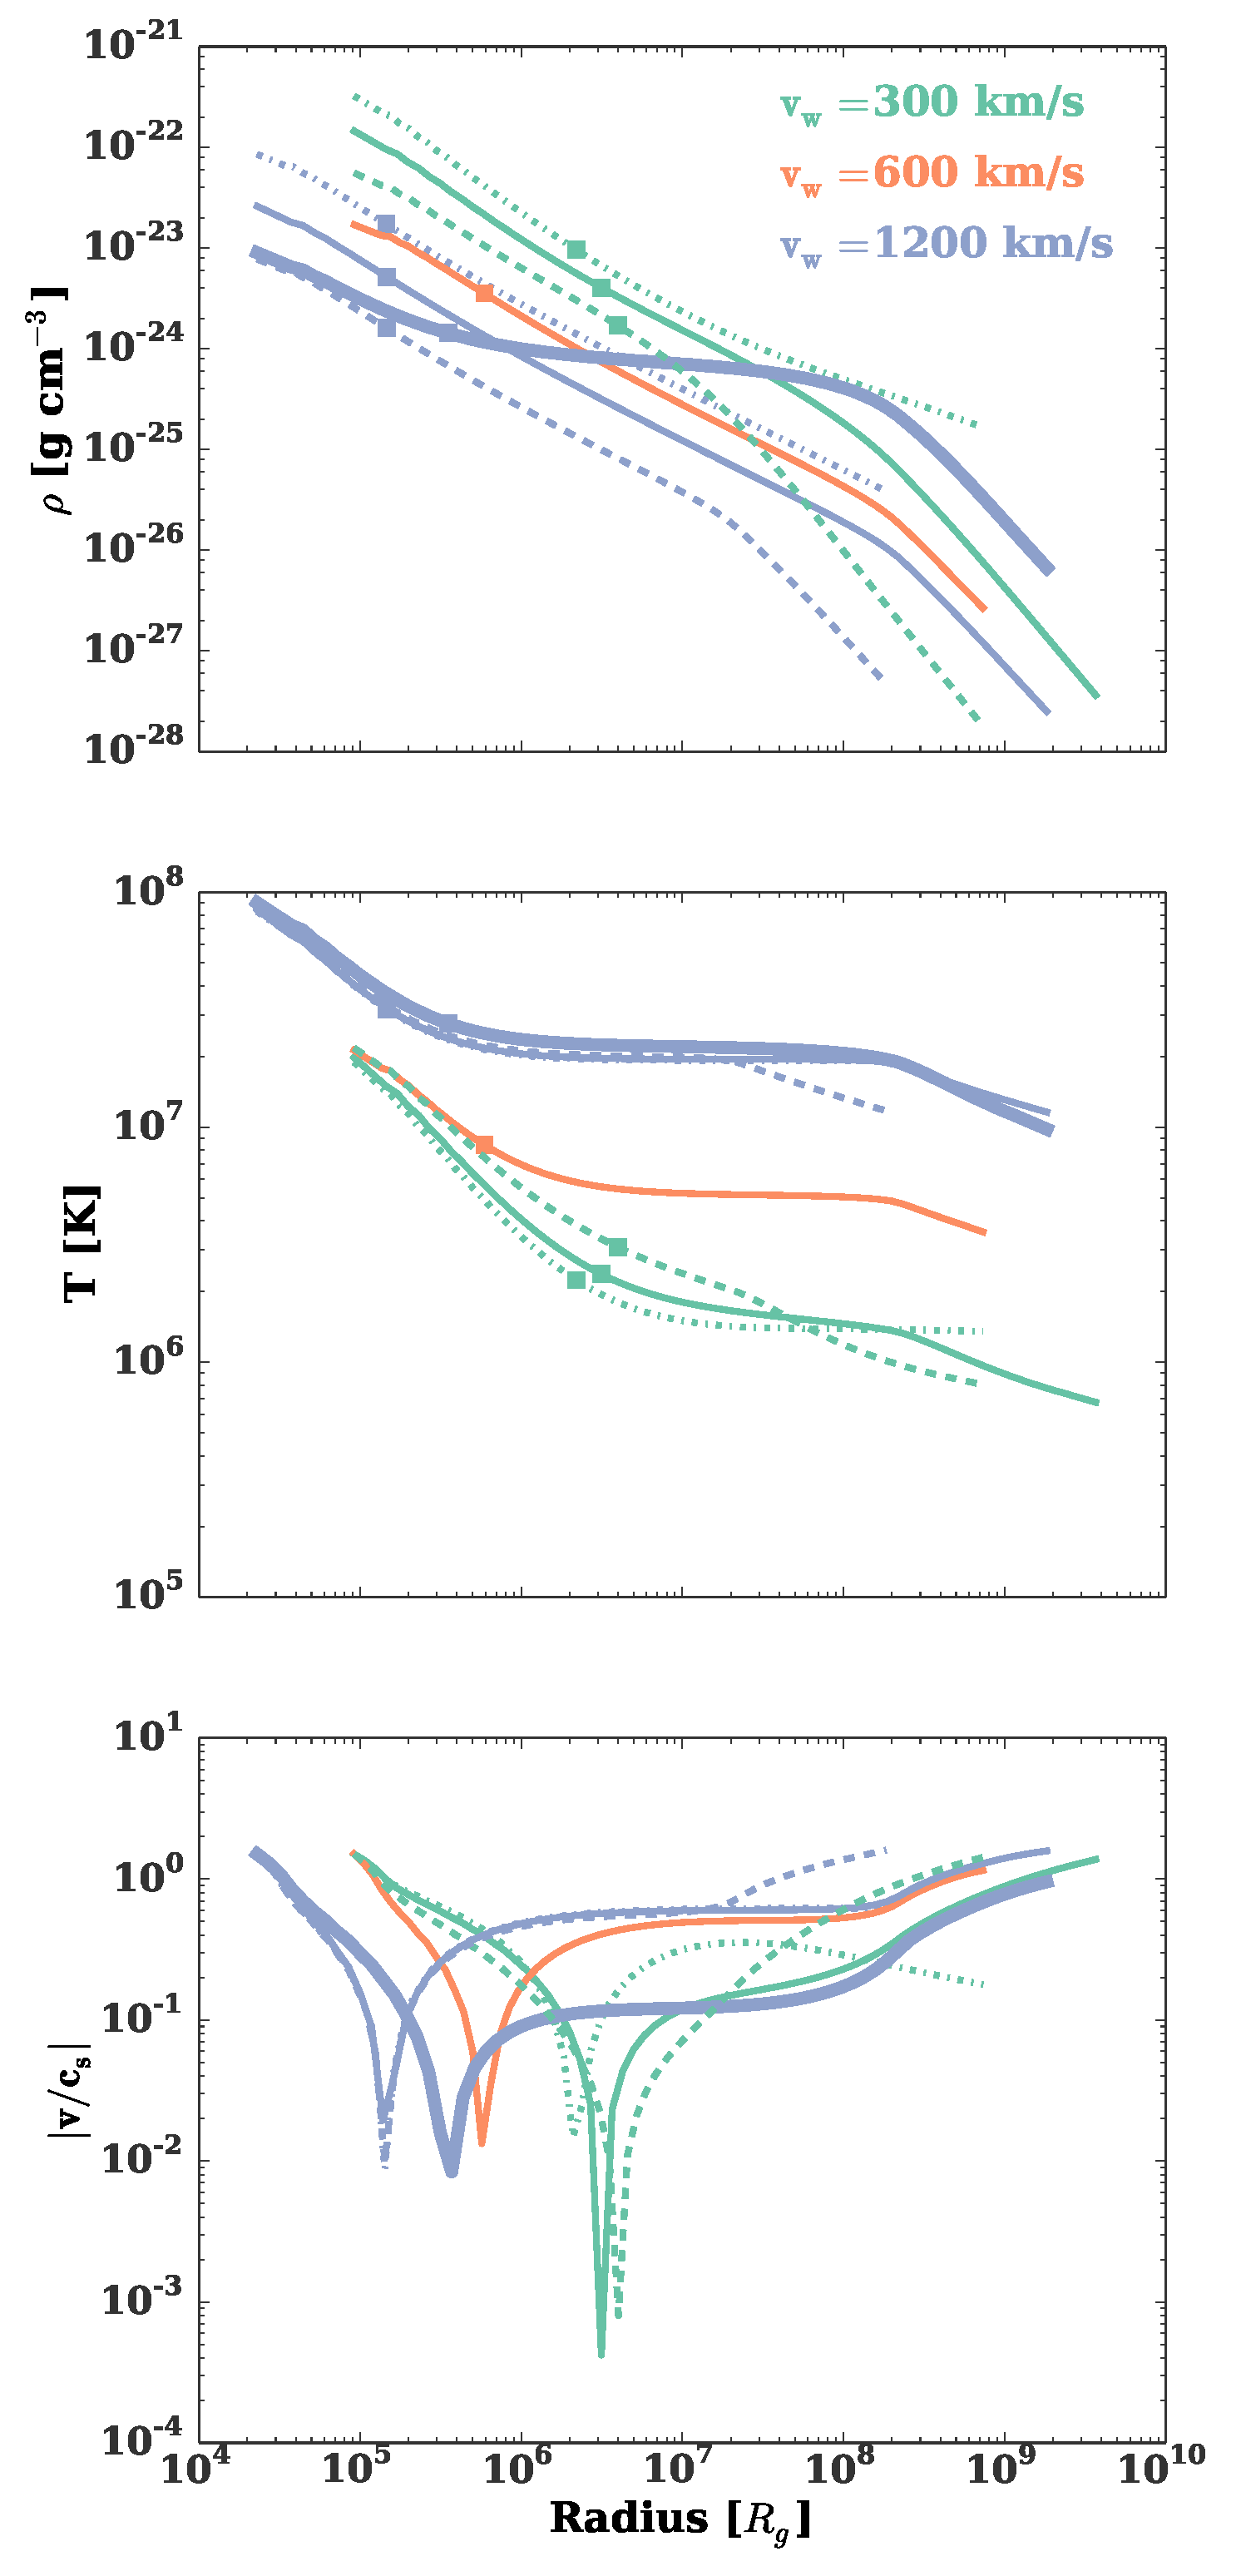
\includegraphics[width=\columnwidth]{profiles.eps}
  \caption{\label{fig:profiles}Radial profiles of the CNM density
    ({\it top}), temperature ({\it middle}), and velocity ({\it bottom}),
    calculated for a representative sample of galaxies.  Different colors
    denote different values of the effective wind heating rate,
    $\vwO=1200$ km s$^{-1}$ ({\it blue}), $\vwO$=600 km s$^{-1}$ ({\it
      orange}), and 300 km s$^{-1}$ ({\it green}).  Different
    linestyles correspond to different values of $\Mbh$, $\Mbh=10^6
    \Msun$ ({\it dot-dashed}), $\Mbh=10^7 \Msun$ ({\it solid}), and
    $\Mbh=10^8 \Msun$ ({\it dashed}). Thin lines correspond to cusp
    galaxies ($\Gamma$=0.8) and thick lines correspond to core
    galaxies ($\Gamma$=0.1). Squares mark the location of
    the stagnation radius for each solution.
 }
\end{figure}

  \subsection{Angular Momentum}
  \label{sec:rotation}

  Our spherically symmetric model neglects the effects of angular
  momentum on the gas evolution.  However, all galaxies possess some
  net rotation, resulting in centrifugal forces becoming important at
  some radius $r_{\rm circ} = l^{2}_{r_{s}}/(GM_{\bullet})$.  Here
  $l_{r_{s}} = \langle r V_{\phi}\rangle |_{r_s}$ is the stellar
  specific angular momentum near the stagnation radius, from which
  most of the accreted mass originates, where $V_{\phi}$ is the
  stellar azimuthal velocity.

  \citet{EmsellemCappellari+:2007a} use two-dimensional kinematic data
  to measure the ratio of ordered to random motion in a sample of
  early type galaxies, which they quantify at each galactic radius $R$
  by the parameter
  \begin{align}
    \lambda_R \equiv \frac{\langle r|V|\rangle}{\langle R\sqrt{V^2+\sigma^2}\rangle} \underset{R \ll r_{\rm soi}}\sim \frac{V_{\phi}}{\sigma},
  \end{align}
  where $\sigma$ is the velocity dispersion and the brackets indicate
  a luminosity-weighted average.  The circularization radius of the
  accretion flow can be written in terms of $\lambda_R$ as

\begin{equation}
\frac{r_{\rm circ}}{r_{s}} \approx \frac{r_{s}}{r_{\rm soi}}\lambda_{R}^{2} \lesssim \lambda_{R}^{2},
\label{eq:rcirc}
\end{equation}
where we have used the definition $r_{\rm soi} \equiv
GM_{\bullet}/\sigma^{2}$ and in the second inequality have assumed
that $r_{\rm s} \lesssim r_{\rm soi}$, a condition which is satisfied
for the thermally-stable solutions of interest.

\citet{EmsellemCappellari+:2007a} (their Fig.~2) find that $\lambda_R$
is generally $< 0.1$ on radial scales $<$ 10 per cent of the galaxy
half-light radius and that $\lambda_R$ decreases with decreasing $R$ interior to this point.  From equation (\ref{eq:rcirc}) we thus conclude that $r_{\rm
  circ} \lesssim 0.01r_{s}$, i.e.~that gas will circularize well
inside the inner sonic point of the flow (typically located at $r\lsim
0.1r_{\rm s}$; Fig.~\ref{fig:profiles}).  Angular momentum should only
become dynamically important for thermally stable flows in a region
that is causally disconnected from the outer part of the flow where
the mass accretion rate is determined.


\section{Numerical Results}
\label{sec:numerical}

\begin{table*}
\begin{threeparttable}
%\centering
\begin{minipage}{18cm}
\caption{Summary of Numerical Solutions}
\begin{tabular}{lccccccccc}
  \hline
  {$M_{\bullet}$} & {$v_{w}$} & {$r_b^{(b)}$} &  $\Gamma$ &  $r_{\rm
    s}/r_{\rm soi}$ &  {$\left(\frac{\dot{M}}{\dot{M}_{\rm
          edd}}\frac{0.2}{\eta}\right)_{r_{s}}^{(c)}$} &
  {$\left(\dot{q}_{\rm heat}/|\dot{q}_{\rm rad}|\frac{0.2}{\eta}\right)_{r_s}^{(d)}$} & Issues? \\
  ($M_{\odot}$) & (km s$^{-1}$) & (pc) &- & - & - &  & \\ 
\hline
 & & & Cusp Galaxies, $\Gamma^{(a)} = 0.8$ & & & & & \\
$    10^{ 6 }$ & 300 & 0.8 & 100 & 0.14 & $ 6.4 \times 10^{ -5 }$ & 17 \\
... & 600 & 0.8 & 100 & $ 3.4 \times 10^{ -2 }$ & $ 1.1 \times 10^{ -5 }$ & $ 1.6 \times 10^{ 3 }$ \\
... & 1200 & 0.8 & 100 & $ 8.2 \times 10^{ -3 }$ & $ 1.9 \times 10^{ -6 }$ & $ 7.2 \times 10^{ 4 }$ \\
$    10^{ 7 }$ & 300 & 0.8 & 25 & 0.65 & $ 3.9 \times 10^{ -4 }$ & 1.8 \\
... & ... & 0.8 & 50 & 0.65 & $ 3.9 \times 10^{ -4 }$ & $\mathbf{0.82}$ \\
... & ... & 0.8 & 100 & 0.83 & $ 5.2 \times 10^{ -4 }$ & $\mathbf{0.33}$ \\
... & ... & 0.8 & 200 & 0.91 & $ 5.9 \times 10^{ -4 }$ & $\mathbf{0.18}$ \\
... & ... & 0.8 & 400 & 2.3 & $ 1.8 \times 10^{ -3 }$ & $\mathbf{ 1.9 \times 10^{ -2 }}$ \\
... & 600 & 0.8 & 25 & $ 8.9 \times 10^{ -2 }$ & $ 3.6 \times 10^{ -5 }$ & $ 4.4 \times 10^{ 2 }$ \\
... & ... & 0.8 & 100 & $ 8.9 \times 10^{ -2 }$ & $ 3.6 \times 10^{ -5 }$ & $ 4.4 \times 10^{ 2 }$ \\
... & 1200 & 0.8 & 100 & $ 2.1 \times 10^{ -2 }$ & $ 6.4 \times 10^{ -6 }$ & $ 2.4 \times 10^{ 4 }$ \\
$    10^{ 8 }$ & 300 & 0.8 & 25 & 1.3 & $ 9.4 \times 10^{ -4 }$ & $\mathbf{1}$ \\
... & ... & 0.8 & 50 & 2.1 & $ 1.6 \times 10^{ -3 }$ & $\mathbf{0.19}$ \\
... & ... & 0.8 & 100 & 3.8 & $ 3.3 \times 10^{ -3 }$ & $\mathbf{ 2.2 \times 10^{ -2 }}$ \\
... & ... & 0.8 & 200 & 7.3 & $ 7.2 \times 10^{ -3 }$ & $\mathbf{ 2.1
  \times 10^{ -3 }}$ \\
... & 450 & 0.8 & 100 & 0.72 & $ 4.4 \times 10^{ -4 }$ & 4 \\
...$^{\dagger}$ & ... & 0.8 & 100 & 3.3 & $ 2.8 \times 10^{ -3 }$ & $\mathbf{2.8}$\\
... & 600 & 0.8 & 25 & 0.26 & $ 1.3 \times 10^{ -4 }$ & $ 1.1 \times 10^{ 2 }$ \\
... & ... & 0.8 & 100 & 0.28 & $ 1.5 \times 10^{ -4 }$ & 76 \\
...$^{\dagger}$ & ... & 0.8 & 100 & 0.29 & $ 1.5 \times 10^{ -4 }$ &
70 \\
...$^{\ddagger}$ & ... & 0.8 & 100 & 0.31 & $ 1.6 \times 10^{ -4 }$ & 73 \\
... & ... & 0.8 & 200 & 0.3 & $ 1.5 \times 10^{ -4 }$ & 67 \\
... & ... & 0.8 & 400 & 0.31 & $ 1.6 \times 10^{ -4 }$ & 58 \\
... & 1200 & 0.8 & 100 & $ 5.4 \times 10^{ -2 }$ & $ 2.0 \times 10^{
  -5 }$ & $ 7.2 \times 10^{ 3 }$ \\
  \hline
 & & & Core Galaxies, $\Gamma = 0.1$ & & & & & & \\
$    10^{ 6 }$ & 600 & 0.1 & 25 & $ 9.9 \times 10^{ -2 }$ & $ 8.2
\times 10^{ -6 }$ & 99 & Conv\\
... & ... & 0.1 & 50 & 0.34 & $ 8.5 \times 10^{ -5 }$ & $\mathbf{0.45}$ \\
... & 1200 & 0.1 & 25 & $ 1.7 \times 10^{ -2 }$ & $ 2.9 \times 10^{ -7 }$ & $ 1.4 \times 10^{ 5 }$ \\
... & ... & 0.1 & 50 & $ 1.7 \times 10^{ -2 }$ & $ 2.9 \times 10^{ -7 }$ & $ 1.4 \times 10^{ 5 }$ \\
... & ... & 0.1 & 100 & $ 1.7 \times 10^{ -2 }$ & $ 2.9 \times 10^{ -7 }$ & $ 1.4 \times 10^{ 5 }$ \\
$    10^{ 7 }$ & 600 & 0.1 & 25 & 0.24 & $ 4.3 \times 10^{ -5 }$ & 41 \\
... & ... & 0.1 & 50 & 0.57 & $ 2.3 \times 10^{ -4 }$ & $\mathbf{0.38}$ \\
... & 1200 & 0.1 & 25 & $ 4.4 \times 10^{ -2 }$ & $ 1.8 \times 10^{ -6 }$ & $ 2.2 \times 10^{ 4 }$ \\
... & ... & 0.1 & 50 & $ 4.7 \times 10^{ -2 }$ & $ 2.0 \times 10^{ -6 }$ & $ 1.7 \times 10^{ 4 }$ \\
... & ... & 0.1 & 100 & $ 5.3 \times 10^{ -2 }$ & $ 2.5 \times 10^{ -6 }$ & $ 9.8 \times 10^{ 3 }$ \\
$    10^{ 8 }$ & 600 & 0.1 & 25 & 0.39 & $ 1.1 \times 10^{ -4 }$ & 31 \\
... & ... & 0.1 & 50 & 0.66 & $ 3.0 \times 10^{ -4 }$ & 3 \\
... & ... & 0.1 & 100 & 2.6 & $ 4.0 \times 10^{ -3 }$ & $\mathbf{ 5.7 \times 10^{ -3 }}$ \\
... & 1200 & 0.1 & 25 & 0.1 & $ 8.4 \times 10^{ -6 }$ & $ 5.6 \times 10^{ 3 }$ \\
... & ... & 0.1 & 50 & 0.11 & $ 9.8 \times 10^{ -6 }$ & $ 4.0 \times 10^{ 3 }$ \\
... & ... & 0.1 & 100 & 0.12 & $ 1.2 \times 10^{ -5 }$ & $ 2.4 \times 10^{ 3 }$ \\
... & ... & 0.1 & 200 & 0.16 & $ 2.1 \times 10^{ -5 }$ & $ 6.5 \times 10^{ 2 }$ \\
... & ... & 0.1 & 400 & 3.3 & $ 6.2 \times 10^{ -3 }$ & $\mathbf{ 5.8 \times 10^{ -3 }}$ \\
  \hline

\label{table:models}  
\end{tabular}
\begin{tablenotes}
\item $^{(a)}$ Inner power-law index of stellar Nuker profile.
  $^{(b)}$ Break radius of stellar Nuker profile.  $^{(c)}$Accretion
  rate in Eddington units, normalized to a stellar mass input
  parameter $\eta = 0.2$.  $^{(d)}$Ratio of wind heating rate to
  radiative cooling rate at the stagnation radius.  Thermally unstable
  solutions are shown in bold text.  $\dagger$Calculated with
  radiative cooling included, assuming mass loss parameter $\eta =
  0.2$.  $\ddagger$Calculated with radiative cooling and conductivity
  included, assuming mass loss parameter $\eta = 0.2$ and conductivity
  saturation parameter $\phi = 0.1$ (recall that the
  conductive heat flux saturates to $F_{\rm cond}=5\phi \rho c_s^3$). 
\end{tablenotes}
\end{minipage}
\end{threeparttable}

\end{table*}




%\begin{table*}
%\centering
%\begin{minipage}{18cm}
%\caption{Comparison of numerical solutions with and without
 % cooling. We have chosen $\eta=0.04$, which one would expect for 
  %the average star formation history for $\Mbh=10^8\Msun$ 
 % (see Figures~\ref{fig:eta} {\bf AG-cite star formation history
  %  figure once it is made.}). Note that we have deliberately chosen a solution
  %near our thermal stability threshold where cooling is beginning
  %to become important.
%}
%\begin{tabular}{lccccccccccccc}
%\hline
%{$M_{\bullet,8}$} & {$v_{w}$} & {$\Gamma$} & {$r_b$} & {$\eta$} &
%{$\dot{M}/\dot{M}_{\rm edd}$} & {$(t_{\rm cool}/t_{\rm ff})_{r_s}$} & {comments}\\
%\hline
%1 & 300 & 0.8 & 50.0 & 0.04 & $ 3.3 \times 10^{ -4 }$ & 4.6 &  \\
%1 & 300 & 0.8 & 50.0 & 0.04 & $ 9.1 \times 10^{ -4 }$ & 5.6 & \\
%\hline
%\label{table:models}  
%\end{tabular}
%\end{minipage}
%\end{table*}

Our numerical results, summarized in Table \ref{table:models}, allow us to study a range of CNM properties and to assess the validity of the analytic estimates from the previous section.  Cases for which $\dot{q}_{\rm heat}/|\dot{q}_{\rm rad}|< 1$ at the stagnation radius are marked as `thermally unstable', as are cases for which the stagnation radius diverges and hence could not be resolved, resulting in their calculations being terminated.  

Figure~\ref{fig:profiles} shows profiles of the density $\rho(r)$,
temperature $T(r)$, and radial velocity $|v(r)|$ (expressed in units of the sound speed), for the cusp
($\Gamma=0.8$) solutions within our grid.  As expected, the gas
density increases towards the SMBH $\rho\propto r^{-\densSlope}$ with
$\densSlope\simeq1$, i.e. shallower than the $-3/2$ power law for
Bondi accretion. This power law behavior does not extend
through all radii, however, as the gas density profile has a break coincident
with the location of the break in the stellar light profile ($\rb=100$
pc). The temperature profile is relatively flat at large radii, but
increases as $\propto 1/r^{k}$ interior to the sphere of influence,
where $k\lesssim 1$, somewhat shallower than expected for virialized gas within the black hole sphere of influence.
The inwardly directed velocity increases towards the hole with a profile that is somewhat steeper than the local free-fall velocity $v \propto v_{\rm ff}\propto r^{-1/2}$.  The flow near the stagnation radius is subsonic, but becomes supersonic at two critical points, one located at small radii, $r \lesssim 0.1r_{\rm s}$, and the other located at large radii, $r \gtrsim 10^{3}r_{\rm s}$.  In many cases the supersonic transition is instigated by the transition to a steeper stellar density profile exterior to the outer Nuker break radius, making our solutions near $r_{\rm s}$ also potentially sensitive to the break radius value.
% {\bf BDM: I made this up - in general we need
%   more explanation of what the plots are actually showing, with some
%   physical explanation.}
% AG -- things are not quite approaching Bondi on the inner grid. I
% don't have a good physical explanation yet...

Figure~\ref{fig:stag} shows our results for the stagnation radius
$r_{\rm s}$, expressed in ratio to sphere of influence radius $r_{\rm
  soi}$, with different colors showing different values of $v_{w}$.
Cusp and core galaxies are marked with square and triangles,
respectively.  Shown for comparison are our analytic results
(eq.~[\ref{eq:rs2main}]) with solid and dashed lines for cusp and core
galaxies, respectively, calculated assuming $\densSlope = 1$ and
$\densSlope= 0.6$, respectively (eq.~[\ref{eq:densSlope}]).  Our analytic estimates are found to
provide accurate fits to the numerical results for $v_{\rm w} \gtrsim
\sigma$, but the assumptions leading to these estimates become invalid
for low $v_{\rm w}$ as the stagnation radius diverges to large radii.
For $v_{w} \gg \sigma$ the ratio $\rs/\rsoi$ does not depend
sensitively on break radius $r_{b}$, but the latter has a greater
influence when $v_{w} \lesssim \sigma$.  The three green squares which
are vertically aligned at the same value of $v_{w}/\sigma$ (close to
where the analytic estimate diverges) correspond to models with the
same black hole mass ($\Mbh = 10^7 \Msun$) and heating rate ($v_w =
300$ km s$^{-1}$) but different values of the break radius: $r_{b} = $
50, 100, and 400 pc (from top to bottom).  As $r_{\rm b} \rightarrow
r_{s}$, the effects of the break radius is to the push the stagnation
radius inwards, decreasing the SMBH accretion rate.

 Figure~\ref{fig:mdot_mass} shows the SMBH accretion rate for each of our numerical solutions in Eddington units for different values of $\vwO =$ 300, 600 and 1200 km s$^{-1}$, and for both core ($\Gamma$=0.1) and cusp galaxies ($\Gamma$=0.8).  Shown for comparison is our analytic estimate of $\dot{M}/\dot{M}_{\rm edd}$ from equation (\ref{eq:eddr_analytic}).  For high wind velocities ($v_{w} \gg \sigma$) the stagnation lies well inside the black hole sphere of influence and our analytic estimate provides a good fit to the numerical results.  However, for low wind velocities and/or high $M_{\bullet}$ (large $\sigma$), the numerical accretion rate considerably exceeds the analytic estimate as the stagnation radius diverges to large radii (Fig.~\ref{fig:stag}).  
%% AG: Describe conservation checks to additionally validate the results.

\begin{figure}
  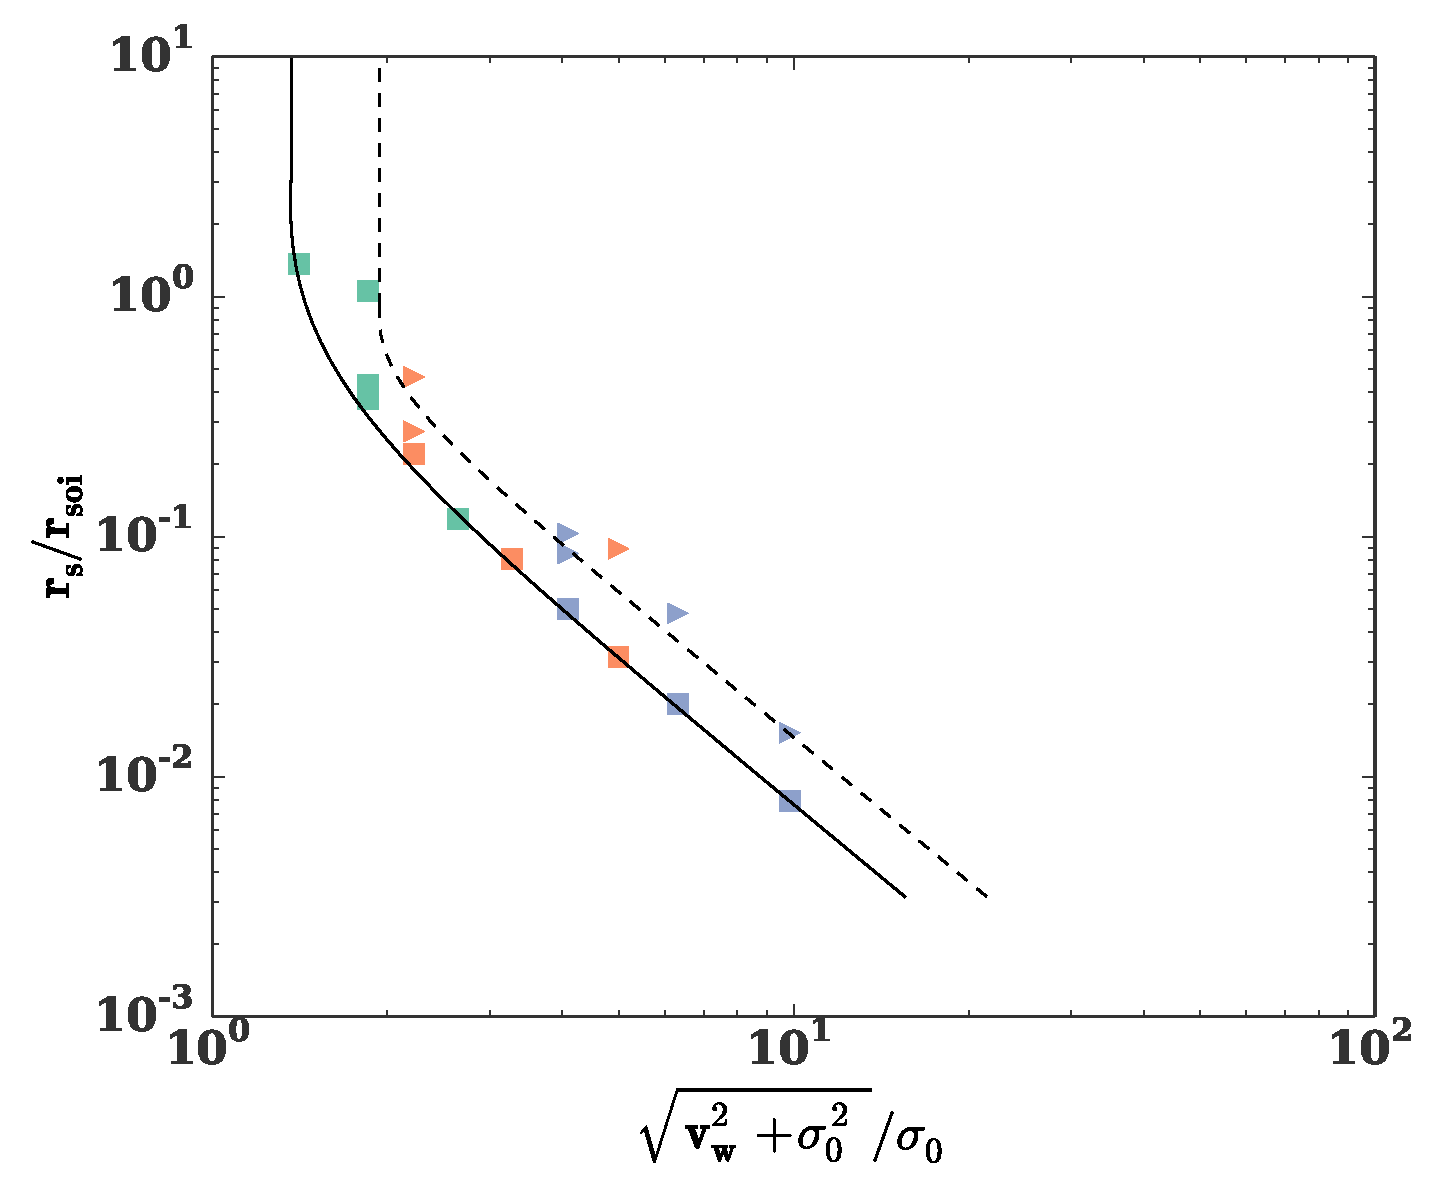
\includegraphics[width=\columnwidth]{rs.eps}
  \caption{\label{fig:stag} \emph{Top panel:} Stagnation radius
    $r_{s}$ in units of the sphere of influence radius $r_{\rm soi}$
    (eq.~[\ref{eq:rsoi}]) for galaxies in our sample as a function of
    the ratio of the effective wind heating rate $v_{w}$ to the
    stellar velocity dispersion $\sigma$.  Green, orange, and blue
    symbols correspond to different values of $v_{w} =$ 300, 600, and
    1200 km s$^{-1}$, respectively.  Squares correspond to cusp
    galaxies ($\Gamma = 0.8$), while triangles correspond to cores
    ($\Gamma = 0.1$). The black curves correspond to the analytic
    prediction from equation (\ref{eq:rs2main}), with solid and dashed
    curves calculated for parameters $\{\Gamma=0.8, \densSlope\simeq1\}$ and
    $\{\Gamma=0.1,\densSlope\simeq0.6\}$, respectively. }
\end{figure}


\begin{figure}
  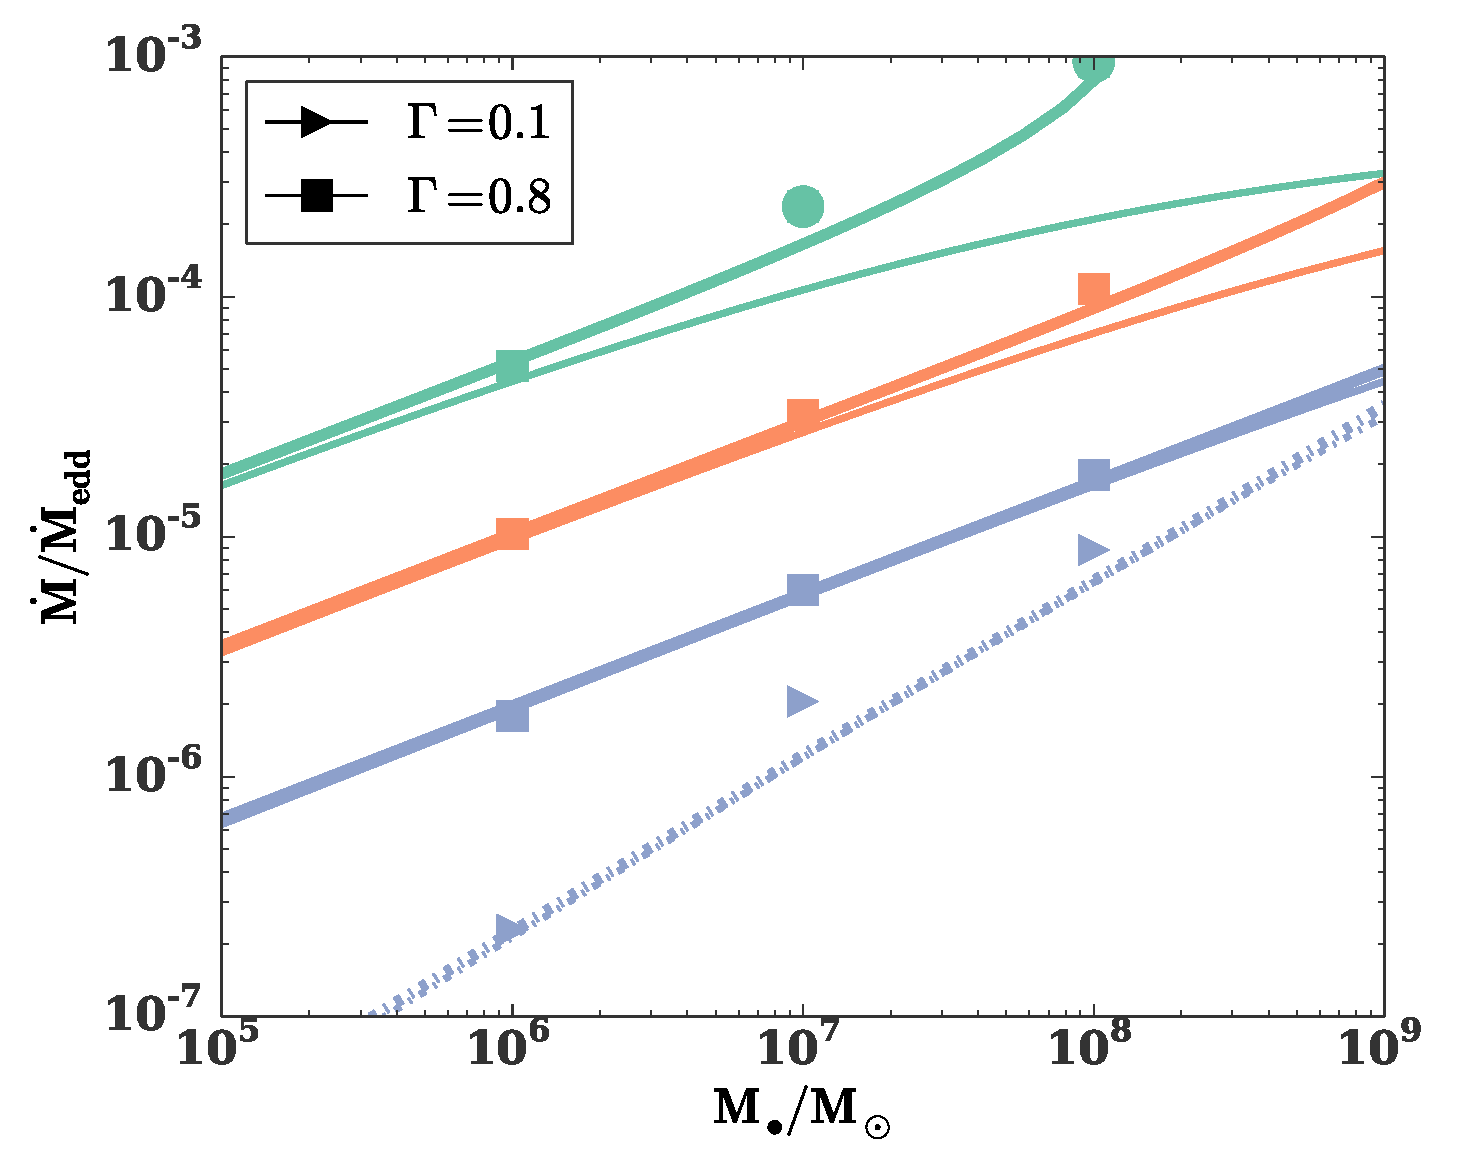
\includegraphics[width=\columnwidth]{mdot_mass.eps}
  \caption{\label{fig:mdot_mass} Accretion rate $\dot{M}/\dot{M}_{\rm edd}$ versus SMBH mass for galaxies in our sample, calculated for different values of the wind heating parameter $\vwO =$ 300 km s$^{-1}$ ({\it green}),
    600 km s$^{-1}$ ({\it orange}), and 1200 km s$^{-1}$ ({\it blue}).
    Squares correspond to cusp galaxies ($\Gamma=0.8$), while
    triangles correspond to cores ($\Gamma$=0.1). Solid and dashed curves correspond to our analytic estimates of $\dot{M}/\dot{M}_{\rm edd}$ (eq.~[\ref{eq:eddr_analytic}]) for cusp and core galaxies, respectively. }
\end{figure}


\begin{figure}
  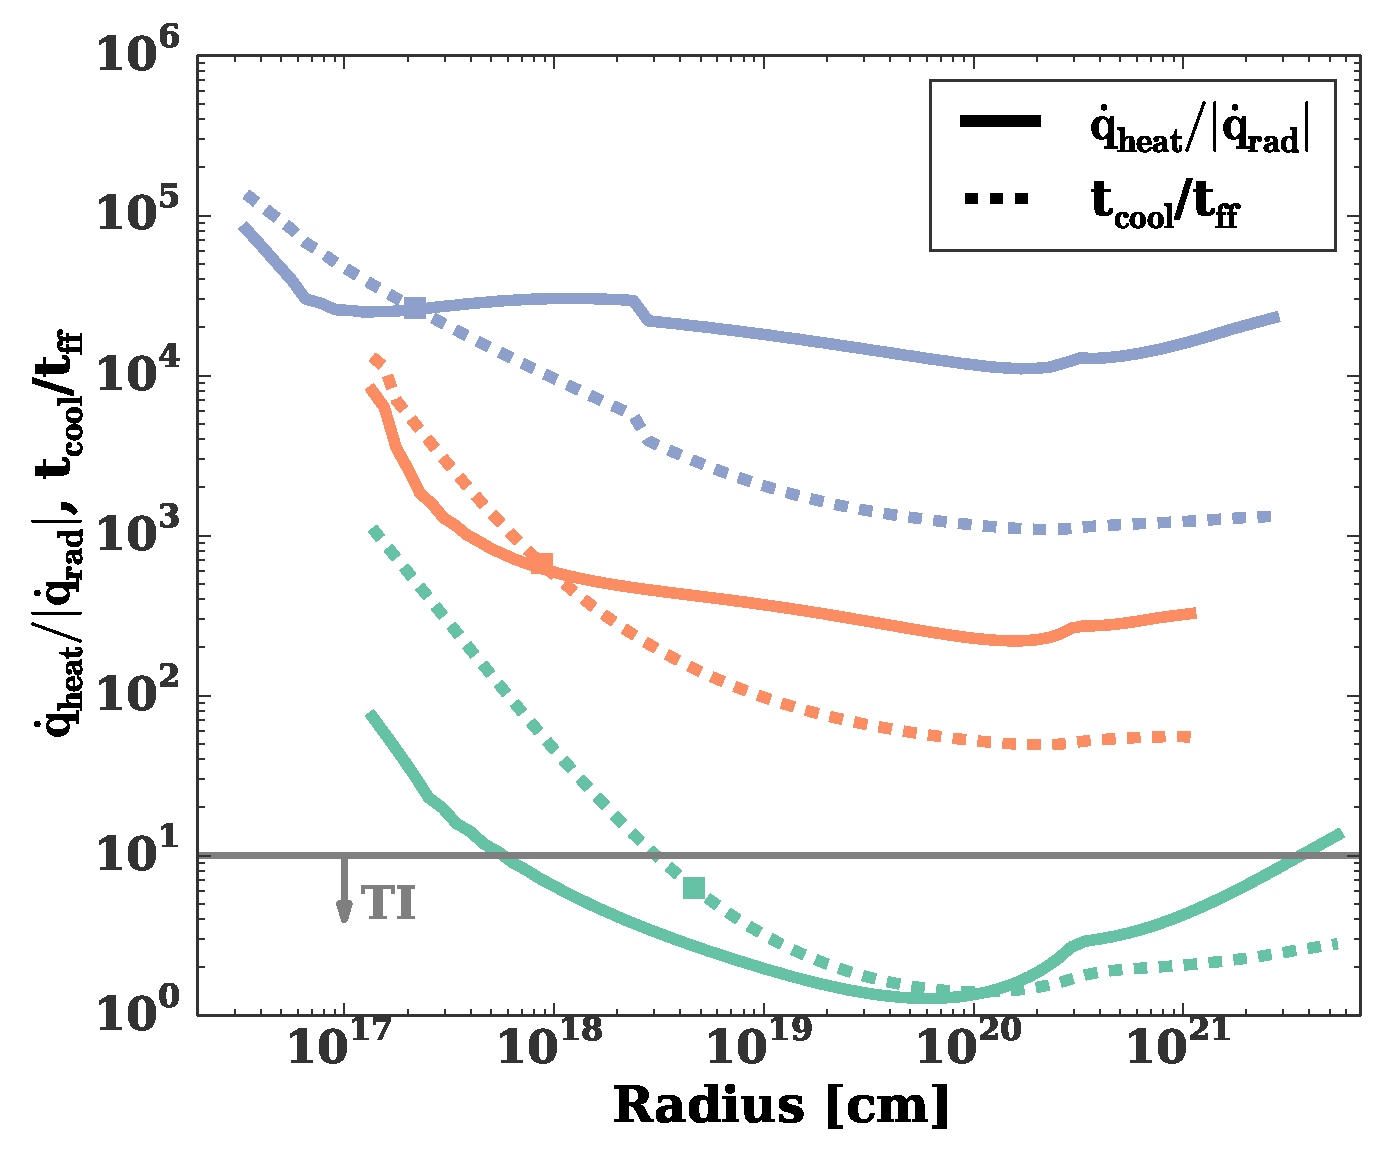
\includegraphics[width=\columnwidth]{cooling.eps}
  \caption{\label{fig:cooling} Ratio of the rate of heating to
radiative cooling, $\dot{q}_{\rm heat}/|\dot{q}_{\rm rad}|$, as a
function of radius (solid lines) for each of our solutions shown in
Figure \ref{fig:profiles}.  Dashed lines show for comparison the ratio
of the cooling to the free-fall timescale $t_{\rm cool}/t_{\rm ff}$.
For high heating rates both ratios are approximately equal at the
stagnation radius (marked as squares).  When $\dot{q}_{\rm
heat}/\dot{q}_{\rm rad} \lesssim 1$ and/or $t_{\rm cool}/t_{\rm ff}
\lesssim 10$, the flow is susceptible thermal instabilities.}
\end{figure}


Fig.~\ref{fig:cooling} shows the ratio of wind heating to radiative
cooling, $\dot{q}_{\rm heat}/|\dot{q}_{\rm rad}|$
(eq.~[\ref{eq:cooling2}] and surrounding discussion) as a function of
radius for our fiducial solutions shown in Figure \ref{fig:profiles}.
For high heating rates of $v_{w} = 600$ and $1200$ km s$^{-1}$ cooling
is unimportant across all radii, while for $v_{w} = 300$ km s$^{-1}$
we see that $\dot{q}_{\rm heat}/|\dot{q}_{\rm rad}|$ and $\tcool/\tff$
can be less than unity, depending on the wind mass loss parameter
$\eta$.  At the stagnation radius, the ratio $\dot{q}_{\rm
  heat}/|\dot{q}_{\rm rad}|$ reaches a value that lies within a factor
of two of its minimum across the entire grid; thus, the value of
$(\dot{q}_{\rm heat}/|\dot{q}_{\rm rad}|)_{r_{s}}$ provides a
diagnostic of thermal instabilty for the entire solution.

Also note that for $v_{w}=600$ and $1200$ km s$^{-1}$ we have that
$\dot{q}_{\rm heat}/|\dot{q}_{\rm rad}| \sim t_{\rm cool}/t_{\rm ff}$
near the stagnation radius.  However, the two ratios diverge from each
other at low heating ($v_{w} \lesssim 300$ km s$^{-1}$) because
equations (\ref{eq:mdot_gas}), (\ref{eq:rhors}) underestimate the true
gas density, which is greater in a subsonic inflow (weak heating) than
in a supersonic outflow (strong heating).

In addition to our standard set of solutions neglecting thermal conduction and cooling, we explore a few test simulations including these effects, as marked by dagger symbols in Table \ref{table:models}.  For solutions which are far from being thermally unstable when cooling is neglected (e.g. $M_{\bullet} = 10^{8}M_{\odot}$, $v_{w} = 600$ km s$^{-1}$, $r_{b} = 100$ pc, $\eta = 0.2$, $\dot{q}_{\rm heat}/|\dot{q}_{\rm rad}| = 76$), the effects of including radiative cooling on the key properties of the flow (stagnation radius, mass accretion rate, $\dot{q}_{\rm heat}/|\dot{q}_{\rm rad}|$ ratio) are small.  However, for solutions in which cooling stability is marginal (e.g. $\dot{q}_{\rm heat}/|\dot{q}_{\rm rad}| \sim $few), including cooling decreases the value of $\dot{q}_{\rm heat}/|\dot{q}_{\rm rad}|$ by a greater fraction.  Likewise, we find that the key properties of solutions including thermal conduction are always minor for our choice of the saturation parameter $\phi = 0.1$, and they act to offset the effects of radiative cooling, i.e. to make the flow more thermally stable (e.g.~\citealt{Zakamska&Narayan03}).  

\section{Sources of Heating}
\label{sec:heating}

Key properties of the flow, such as the SMBH accretion rate and the likelihood of thermal instability depend sensitively on the assumed heating rate $\propto qv_{w}^{2}$.  This section summarizes individual heating sources, providing estimates of the value of
\begin{align}
  v_{w} = \sqrt{\frac{2 t_h \dot{e}}{\eta \rhostar}}
  \label{eq:vw_eff}
\end{align}
for each, where $\dot{e}$ is volumetric heating rate.  

\subsection{Stellar winds} 

Energy and mass input to the CNM by stellar winds is the sum of contributions from main sequence and post-main sequence populations.  At early times following star formation, energy input is dominated by core collapse supernovae and by the fast outflows of Wolf-Rayet stars (e.g., \citealt{VossDiehl+:2009a}).  At later times energy input is dominated by main sequence winds (e.g., \citealt{NaimanSoares-Furtado+:2013a}).  Mass input is also dominated by massive stars for very young stellar populations, but for most stellar ages the slow AGB winds of evolved low-mass stars dominate the mass budget.  

In Appendix \ref{app:windheat} we calculate the wind heating rate from
stellar winds, $v_{\rm w}^{\star}$, and the mass loss parameter,
$\eta$ (eq.~[\ref{eq:q}]), as a function of age, $\tau_{\star}$, of a
stellar population which is formed impulsively (Fig.~\ref{fig:vwImp}).  
At the earliest times ($\tau_{\star} \lesssim 10^{7}$ yr), the wind
heating rate exceeds 1000 km s$^{-1}$, while much later ($\tau_{\star}
\sim t_{\rm h}$) stellar wind heating dominated by main sequence winds
is much lower, $v^{\star}_{\rm w} \sim 50-100 $ km s$^{-1}$.  We show
in $\S\ref{sec:combined}$ that for the case of quasi-continueous star
formation representative of the average star formation history of loss
mass galaxies, the stellar wind heating rate produced by stellar winds
can also be significant, $v_{\rm w}^{\star} \sim 1000$ km s$^{-1}$.  
Stellar winds thus contribute a potentially important source of both
energy and mass for the CNM.  An additional uncertainty in the stellar wind heating rate results from the uncertain thermalization efficiency of massive stellar winds.  We assume this efficiency to be unity, an optimistic assumption which is offset by our neglect of energy input from core collapse supernovae, which contribute an energy comparable to that from massive stellar winds.  

\subsection{Type Ia Supernovae} 

Type Ia supernovae (SNe Ia) represent a potentially important source of heating, which unlike core collapse SNe is present even in an evolved stellar population.  If each Ia supernova injects thermal energy $E_{\rm Ia}$ into the interstellar medium, and the SNe rate (per stellar mass) is given by $R_{\rm   Ia}$, then the resulting volumetric heating rate of $E_{\rm Ia}R_{\rm  Ia}$ produces an effective wind heating parameter (eq.~[\ref{eq:vw_eff}]) of \begin{align} v_{w}^{\rm Ia} =\sqrt{\frac{2 t_h R_{\rm Ia}
E_{\rm Ia}}{\eta}} \label{eq:vw_sne}.
\end{align} The thermal energy injected by each SN Ia, $E_{\rm Ia} \simeq
\epsilon_{\rm Ia} 10^{51}$ erg, depends on the efficiency $\epsilon_{\rm Ia}$
with which the initial blast wave energy is converted into bulk or turbulent
motion instead of being lost to radiation.  \cite{Thornton+98}
estimate a radiative efficiency $\epsilon_{\rm Ia} \sim 0.1$,
depending weakly on surrounding density, but \citet{Sharma+14} argues
that $\epsilon_{\rm Ia}$ can be considerably higher, $\sim 0.4$, if
the SNe occur in a hot dilute medium, as may characterize the circumnuclear medium.  Hereafter we adopt $\epsilon_{\rm Ia} = 0.4$ as fiducial.

The SN Ia rate, $\RateIa$, depends on the age of the stellar population, as it represent the convolution of the star formation rate and the Ia delay time distribution (DTD) divided by the present stellar mass.  In
the limit of impulsive star formation, $\RateIa$ is the DTD evaluated at the time since the star formation episode.  The observationally-inferred DTD (Fig. 1 of \citealt{MaozMannucci+:2012a}) has the
approximate functional form \begin{align}
  R_{\rm Ia} =1.7\times 10^{-14}\left(\tau_{\star}/t_{\rm
      h}\right)^{-1.12} M_{\odot}^{-1}\,{\rm yr^{-1}}
\label{eq:DTD}
  \end{align}
  where $\tau_{\star}$ is the time since star formation.

From equations (\ref{eq:vw_sne}), (\ref{eq:DTD}) we thus estimate that 
  \begin{eqnarray} 
    v_{w}^{\rm Ia} &\approx& 700(\epsilon_{\rm
      Ia}/0.4)^{0.5}(\tau_{\star}/t_{\rm h})^{-0.56}\eta_{0.02}^{-1/2}\,{\rm km
      \,s^{-1}} \nonumber \\
&\approx& 700(\epsilon_{\rm
      Ia}/0.4)^{0.5}(\tau_{\star}/t_{\rm h})^{0.09}\,{\rm km
      \,s^{-1}},
\label{eq:vIa}
  \end{eqnarray}
where the second line assumes $\eta\simeq 0.02 (\tau_{\star}/t_h)^{-1.3}$ for a single burst of star formation (e.g. , \citealt{Ciotti+91}).

The high value of $v_{w}^{\rm Ia}$ implies that Ia SNe represent an
important source of CNM heating.  However, SNe can only be
approximated as supplying heating which is spatially and temporally
homogeneous if the rate of SNe is rapid compared to the characteristic
evolution time of the flow at the radius of interest
(\citealt{ShcherbakovWong+:2014a}).  We define the ``Ia radius"
  \begin{align}
    r_{\rm Ia} \sim \left(\frac{G}{R_{\rm Ia}\sigma}\right)^{1/2} \sim
    38 M_{\bullet,8}^{-0.1}(\tau_{\star}/t_{\rm h})^{0.56}\,{\rm pc}
    \label{eq:rIa}
  \end{align}
  as the location exterior of which the time interval between
  subsequent supernovae $\tau_{\rm Ia} \sim (M_{\rm enc}R_{\rm
    Ia})^{-1} \sim G/(r\sigma^{2}R_{\rm Ia})$ exceeds the local
  dynamical timescale $t_{\rm dyn} \sim r/\sigma$, where we again
  adopt the Ia rate for an old stellar population and in the final
  equality we estimate the velocity dispersion using the
  $M_{\bullet}-\sigma$ relationship (eq.~[\ref{eq:Msigma}]).

Assuming that $v_{w}^{\rm Ia} \gg \sigma$ then by substituting
$v_{w}^{\rm Ia}$ (eq.~\ref{eq:vIa}) into equation (\ref{eq:rs_simple})
for the stagnation radius, we find that

\begin{align}
  \left.\frac{r_{\rm Ia}}{r_{\rm s}}\right|_{\rm v_{w}^{\rm Ia}}&\approx
  \begin{cases}
    8\, \eta_{0.02}^{-1} M_{\bullet,8}^{-1.1}(\epsilon_{\rm
     Ia}/0.4) (\tau_{\star}/t_{\rm h})^{-0.56}  & {\rm core}\\
    17\, \eta_{0.02}^{-1} M_{\bullet,8}^{-1.1}(\epsilon_{\rm
     Ia}/0.4) (\tau_{\star}/t_{\rm h})^{-0.56} &{\rm cusp}\\
   \end{cases} \nonumber\\
 &\approx 
 \begin{cases}
    8\, M_{\bullet,8}^{-1.1}(\epsilon_{\rm
     Ia}/0.4) (\tau_{\star}/t_{\rm h})^{0.74}  & {\rm core}\\
    17\, M_{\bullet,8}^{-1.1}(\epsilon_{\rm
     Ia}/0.4) (\tau_{\star}/t_{\rm h})^{0.74} &{\rm cusp}\\
   \end{cases}
\label{eq:rIars}
\end{align}
If $r_{\rm Ia} \gg r_{\rm s}$, then SN Ia heating can only be
approximated as a steady heating source near the stagnation radius for
extremely massive SMBHs with $M_{\bullet} \gtrsim 10^9 \Msun$ or in
the case of a very young stellar population ($\tau_{\star} \ll t_{\rm
h}$).  

%On the other hand, equation (\ref{eq:rIars}) may underestimate
%the importance of Ia heating because $r_{\rm Ia}/r_{\rm s}$ will be
%substantially smaller than its value estimated using $v_{w}^{\rm Ia}$
%if the heating rate excluding SN Ia is less than this.

Even if SN Ia are rare near the stagnation radius, they may cap the
SMBH accretion rate by periodically blowing gas out of the nucleus of
low mass galaxies.  Between successive supernovae, stars release a
gaseous mass $M_{\rm g} \approx \eta M_{\star}\tau_{\rm Ia}/t_{\rm h}$
interior to the Ia radius, which is gravitationally bound to the SMBH
by an energy $E_{\rm bind} \sim M_{\rm g}\sigma^{2}f^{2}$  {\bf BDM: update discussion}.  Thus, according
to the above definitions, $E_{\rm Ia}/E_{\rm bind} \sim (v_{w}^{\rm
  Ia})^{2}/2\sigma^{2} \gtrsim 1$.  Hence, SN Ia are in principle
capable of dynamically clearing out gas from radii $\sim r_{\rm Ia}
\gtrsim r_{\rm s}$, at least for low mass BHs with $\sigma \ll v^{\rm
  Ia}_{w}$.  Thus, even in cases when heating is sufficiently weak
that the stagnation radius formally exceeds $r_{\rm Ia}$, the
accretion rate is limited to a maximum value,
\begin{eqnarray}
\frac{\dot{M}_{\rm Ia}}{\dot{M}_{\rm edd}} &\approx& \frac{\eta M_{\bullet}}{\dot{M}_{\rm edd} t_{\rm h}}\left(\frac{R_{\rm Ia}}{R_{\rm soi}}\right)^{2-\Gamma} \approx \nonumber \\
 && \begin{cases}
    4.5 \times 10^{-4} M_{\bullet,8}^{-1.33}(\tau_{\star}/t_{\rm h})^{-0.2}
   & \text{core} \\
    2.2 \times 10^{-4} \Mbheight^{-0.84}(\tau_{\star}/t_{\rm h})^{-0.6}   & \text{cusp},
  \end{cases}
  \label{eq:eddr_Ia}
\end{eqnarray}
obtained substituting the Ia radius $r_{\rm Ia}$ (eq.~[\ref{eq:rIa}]) for $r_{\rm s}$ in the derivation leading to our estimate of $\dot{M}$ (eq.~[$\ref{eq:eddr_analytic}$]).  Note that $\dot{M}_{\rm Ia}$ usually exceeds the maximum accretion rate for a thermally stable flow $\dot{M}_{\rm TI}$ (eq.~[\ref{eq:Mdotmax}]), implying that dynamical `blow-out' from SNe Ia cannot alone prevent cooling instabilities in the nuclei of low mass galaxies.  Also note that Ia supernovae only cap the accretion rate to this maximum value if the gas feeding the black hole is supplied by local stellar mass loss: the gaseous mass can become much greater if the nucleus is fed externally, e.g. due to a galaxy merger or to cooling flows developing within the galaxy over much longer timescales (e.g.~\citealt{Ciotti&Ostriker07}). 



\subsection{Millisecond Pulsars}
 Energy injection from the spin-down of millisecond pulsars (MSPs) is a potentially
important heating source.  If the number of MSPs per unit stellar mass
is $n_{\rm msp}$ and each contributes on average a spin-down
luminosity $\bar{L}_{\rm sd}$, then the resulting heating per unit
volume $\dot{e} \approx \bar{L}_{\rm sd}n_{\rm msp}\epsilon_{\rm msp}$ results in an
effective heating rate (eq.~ [\ref{eq:vw_eff}]) of 
\begin{eqnarray} v_{w}^{\rm MSP} \sim
30\left(\frac{\epsilon_{\rm msp}}{0.1}\right)^{1/2}\left(\frac{\bar{L}_{\rm
sd}}{10^{34}\,{\rm erg\,s^{-1}}}\right)^{1/2} \eta_{0.02}^{-1/2}\,{\rm
km\,s^{-1}},
 \label{eq:vmsp}
  \end{eqnarray} 
where $\epsilon_{\rm msp}$ is the thermalization efficiency of
the wind, normalized to a value $\lesssim 0.1$ based on that inferred by modeling the interstellar media of globular clusters
\citep{NaimanSoares-Furtado+:2013a}.  Our numerical estimate assumes a
pulsar density $n_{\rm msp} \sim 3 \times 10^{-40} $ MSPs g$^{-1}$, calculated from the estimated $\sim 30,000$ MSPs in the Milky Way (\citealt{Lorimer13}) of stellar mass $\approx 6\times 10^{10}M_{\odot}$.

Based on the ATNF radio pulsar catalog (\citealt{Manchester+05}), we estimate the average spin-down luminosity of millisecond pulsars in the field to be $\bar{L}_{\rm sd} \sim 10^{34}$ erg s$^{-1}$, resulting in $v_{w}^{\rm MSP} \lesssim 30$ km s$^{-1}$ for $\eta \gtrsim 0.02$.  For higher spin-down
luminosities, $L_{\rm sd}\simeq 10^{35}$ ergs s$^{-1}$ characteristic
of some Fermi-detected pulsars, then the higher value of $v_{w}^{\rm MSP}
\lesssim 300$ km s$^{-1}$ makes MSP heating in principle important
under the most optimistc assumptions $\epsilon_{\rm msp} = 1$ and $\eta = 0.02$.  On the other hand, it seems likely that the stellar binaries giving rise to MSPs could be disassociated by stellar interactions in the dense nuclear cluster, reducing the numbers of MSPs as compared to the field population estimate above.  


\subsection{SMBH Feedback}

Feedback from accretion onto the SMBH represents an important source of heating which, however, is also the most difficult to quantify (e.g., \citealt{Brighenti&Mathews03}, \citealt{DiMatteo+05}; \citealt{Kurosawa&Proga09}; \citealt{Fabian12} for a recent review).  A key difference between AGN heating and the other sources discussed thus far is its dependence on the SMBH accretion rate $\dot{M}$, which is itself a function of the heating rate (eq.~[\ref{eq:mdot_analytic}]).  

\subsubsection{Compton Heating}

There are two types of SMBH feedback: kinetic and radiative.  Radiative feedback is potentially effective even in low luminosity AGN via Compton heating (e.g., \citealt{Sazonov+04}, \citealt{Ciotti+10}), which provides a volumetric heating rate (\citealt{Gan+14})
\begin{align}
\dot{e} = 4.1\times 10^{-35}n^{2}\xi T_{\rm C}\,{\rm erg\,cm^{-3}\,s^{-1}},
\end{align}
where $\xi = L/n r^{2}$ is the ionization parameter and $L$ is the SMBH luminosity with Compton temperature $T_{\rm C} \sim 10^{9}$ K $\gg T$ (e.g., \citealt{Ho99}, \citealt{Eracleous+10}).  

The importance of Compton heating can be estimated by assuming the SMBH
radiates with a luminosity $L = \epsilon \dot{M}c^{2}$, where
$\epsilon$ is the radiative efficiency and where $\dot{M}$ is
estimated from equation (\ref{eq:mdot_analytic}).  Then using
equations (\ref{eq:rs_simple}), (\ref{eq:mdot_analytic}),
(\ref{eq:rhors}), (\ref{eq:rhostarrs}) we calculate that from equation
(\ref{eq:vw_eff}) that the effective heating rate at the stagnation radius is given by
\begin{align} v_{w}^{\rm C} \simeq
  \begin{cases} 27 \eta_{0.02}^{0.5}T_{\rm
C,9}^{0.5}\epsilon_{-2}^{0.5} M_{\bullet,8}^{0.38}v_{500}^{-1.4}\,{\rm
km\,s^{-1}} &, \text{core}\\ 30 \eta_{0.02}^{0.5}T_{\rm
C,9}^{0.5}\epsilon_{-2}^{0.5} M_{\bullet,8}^{0.24}v_{500}^{-0.7}\,{\rm
km\,s^{-1}} &, \text{cusp},
  \end{cases}
  \label{eq:vC}
\end{align} where $T_{C,9} = T_{C}/10^{9}$ K and $\epsilon_{-2} =
\epsilon/0.01 \sim 1$.  We caveat that, unlike
stellar wind heating, Compton heating depends on radius, scaling as
$v_{w}^{\rm C}(r) \propto (n^{2}\xi/\rho_{\star})^{1/2} \propto
r^{(\Gamma-\densSlope-1)/2}$, i.e. $\propto r^{-0.6}$ and $\propto r^{-0.75}$
for core ($\Gamma = 0.8$; $\densSlope \simeq 1$) and cusp ($\Gamma = 0.1$;
$\densSlope \simeq 0.6$) galaxies, respectively.  Our model's assumption that the heating
parameter be radially constant is not satisfied, but this variation is sufficiently weak that it should not significantly alter
our conclusions.

If Compton heating acts alone, i.e. $\tilde{v}_{w} = v_{w}^{C}$, then solving equation
(\ref{eq:vC}) for $\tilde{v}_{\rm w}$ yields
\begin{align} v_{w}^{\rm C} \simeq
  \begin{cases} 150 \eta_{0.02}^{0.21}T_{\rm
C,9}^{0.21}\epsilon_{-2}^{0.21} M_{\bullet,8}^{0.16}\,{\rm km\,s^{-1}}
&, \text{core}\\ 96 \eta_{0.02}^{0.29}T_{\rm
C,9}^{0.29}\epsilon_{-2}^{0.29} M_{\bullet,8}^{0.14}\,{\rm km\,s^{-1}}
&, \text{cusp},
  \end{cases}
  \label{eq:vC2}
\end{align} 
Compton heating can thus be significant in young stellar populations with relatively high mass loss rates, e.g. $v_{w}^{\rm C} \gtrsim 300$ km s$^{-1}$ for $\eta \gtrsim 1$.  The mass accretion rate corresponding to the state where Compton heating limits the average accretion rate is given by substituting equation (\ref{eq:vC2}) into equation (\ref{eq:eddr_analytic}):
\begin{align}
\frac{\dot{M}_{C}}{\dot{M}_{\rm edd}} \approx 
\begin{cases} 3\times 10^{-3} \eta_{0.02}^{0.20}T_{\rm
C,9}^{-0.8}\epsilon_{-2}^{-0.8} M_{\bullet,8}^{0.15}
&, \text{core}\\ 8\times 10^{-4} \eta_{0.02}^{0.30}T_{\rm
C,9}^{-0.7}\epsilon_{-2}^{-0.7} M_{\bullet,8}^{0.14}
&, \text{cusp},
  \end{cases}
  \label{eq:MdotCa}
\end{align}
If the accretion luminosity $\epsilon = 10 \dot{M}/\dot{M}_{\rm edd}$
depends on the Eddington ratio as predicted by some models for
radiatively inefficient accretion flows (\citealt{Narayan&Yi95};
\citealt{Narayan+98}; \citealt{XieYuan:2012a}), then the Compton-limited accretion rate becomes
\begin{align}
\frac{\dot{M}_{C}}{\dot{M}_{\rm edd}} \approx 
\begin{cases} 1.8\times 10^{-2} \eta_{0.02}^{0.11}T_{\rm
C,9}^{-0.44}M_{\bullet,8}^{0.08}
&, \text{core}\\ 8.7\times 10^{-4} \eta_{0.02}^{0.17}T_{\rm
C,9}^{-0.4} M_{\bullet,8}^{0.08}
&, \text{cusp}.
  \end{cases}
  \label{eq:MdotC}
\end{align}
%{\bf  Total efficiency is 10 (mdot/MdotEdd). Everywhere.}


\subsubsection{Kinetic Feedback}

Kinetic feedback results from outflows of energy or momentum from close to the black hole in the form of a disk wind or jet, which deposits its energy as heat, e.g. via shocks or wave dissipation, over much larger radial scales (e.g.~\citealt{McNamara&Nulsen07}; \citealt{Novak+11}; \citealt{Gaspari+12}).  

Assume that the outflow power is proportional to the SMBH accretion rate, $L_{\rm j} =
\epsilon_{\rm j} \dot{M}c^{2}$, where $\epsilon_{\rm j} < 1$ is a jet efficiency factor.  Further assume that this energy is deposited as heat uniformly interior to a radius $r_{\rm heat}$ and volume $V_{\rm heat} \propto r_{\rm
heat}^{3}$.  The resulting volumetric heating rate $e = \epsilon_{\rm
j}\dot{M}c^{2}/V_{\rm heat}$ near the stagnation radius results in a heating parameter given by
\begin{eqnarray} v_{w}^{\bullet} &\approx& \left(\frac{2t_{\rm
h}\epsilon_{\rm j}\dot{M}c^{2}}{V_{\rm heat}\eta
\rho_{\star}|_{r_{s}}}\right)^{1/2} \sim \left(\frac{\epsilon_{\rm
j}\dot{M}c^{2}t_{\rm h}}{\eta M_{\rm enc}}\right)^{1/2} \nonumber \\
&\approx& 300\,{\rm km\,s^{-1}}\,\left(\frac{\epsilon_{\rm j}}{10^{-6}}\right)^{1/2}\left(\frac{r_{\rm s}}{r_{\rm
heat}}\right)^{1-\Gamma/2},
\label{eq:vjet}
\end{eqnarray} 
where we have used the facts that $\dot{M} = \eta M_{\star}|_{r_{\rm s}}/t_{\rm h}$ and, for radii inside the Nuker break radius, $M_{\star}(r) \propto
M_{\bullet}(r/r_{\rm soi})^{2-\Gamma}$ (eq.~[\ref{eq:rhostar}]).  If the bulk of the outflow energy is released near the stagnation radius, then even a small heating efficiency $\epsilon_{\rm j} \gtrsim
10^{-5}$ is sufficient for $v_{w}^{\bullet}$ to exceed other sources of non-accretion powered heating.  However, if this energy is instead deposited over much larger physical scales comparable to the size of the galaxy, i.e. $r_{\rm heat} \gtrsim $ 10 kpc $\sim 10^{4}r_{\rm s}$, then kinetic feedback is unimportant, even for a powerful jet with $\epsilon_{\rm j} \sim 1$.  

Using the results of \citet{Bromberg+11}, the time required for a jet of luminosity $L_{\rm
  j}$ and half opening angle $\theta_{\rm j} = 0.1$ (characteristic of
AGN jets) to propagate through a gaseous mass $M_{\rm g}$ of radius $r$ is estimated to be
\begin{eqnarray}
t_{\rm jet} &\sim& 4000\,{\rm yr}\left(\frac{{L}_{\rm j}}{10^{40}\,\rm erg\,s^{-1}}\right)^{-1/3}\left(\frac{r}{\rm pc}\right)^{2/3}\left(\frac{M_{\rm g}}{10^{8}M_{\odot}}\right)^{1/3} 
\end{eqnarray}
Approximating $M_{\rm g} \sim \dot{M}t_{\rm ff}$, the ratio of the jet escape timescale to the dynamical timescale $t_{\rm dyn} \sim r/\sigma$ is given by
\begin{equation}
\frac{t_{\rm jet}}{t_{\rm dyn}} \sim 7\times 10^{-3}M_{\bullet,8}^{0.13}\left(\frac{\epsilon_{\rm j}}{10^{-6}}\right)^{-1/3},
\end{equation}
independent of $r$.  A jet with power sufficient to appreciably heat the CNM on radial scales $\sim r_{\rm s}$ ($\epsilon_{j} \gtrsim 10^{-6}$) also necessarily has sufficient power to escape the nucler region and propagate to much larger radii.  Slower outflows from the accretion disk, instead of a collimated relativistic jet, may provide a more promising source of feedback in these systems (e.g.~\citealt{Li+13}).    

As in the case of Compton heating, kinetic heating could in principle  `self-regulate' the accretion flow insofar as a lower heating rate results in a higher accretion rate (eq.~[\ref{eq:vjet}]), which in turn may create stronger jet feedback.  However, given the uncertainty in the efficiency of jet heating, we defer a more detailed discussion to $\S\ref{sec:kinetic}$.


\begin{figure}
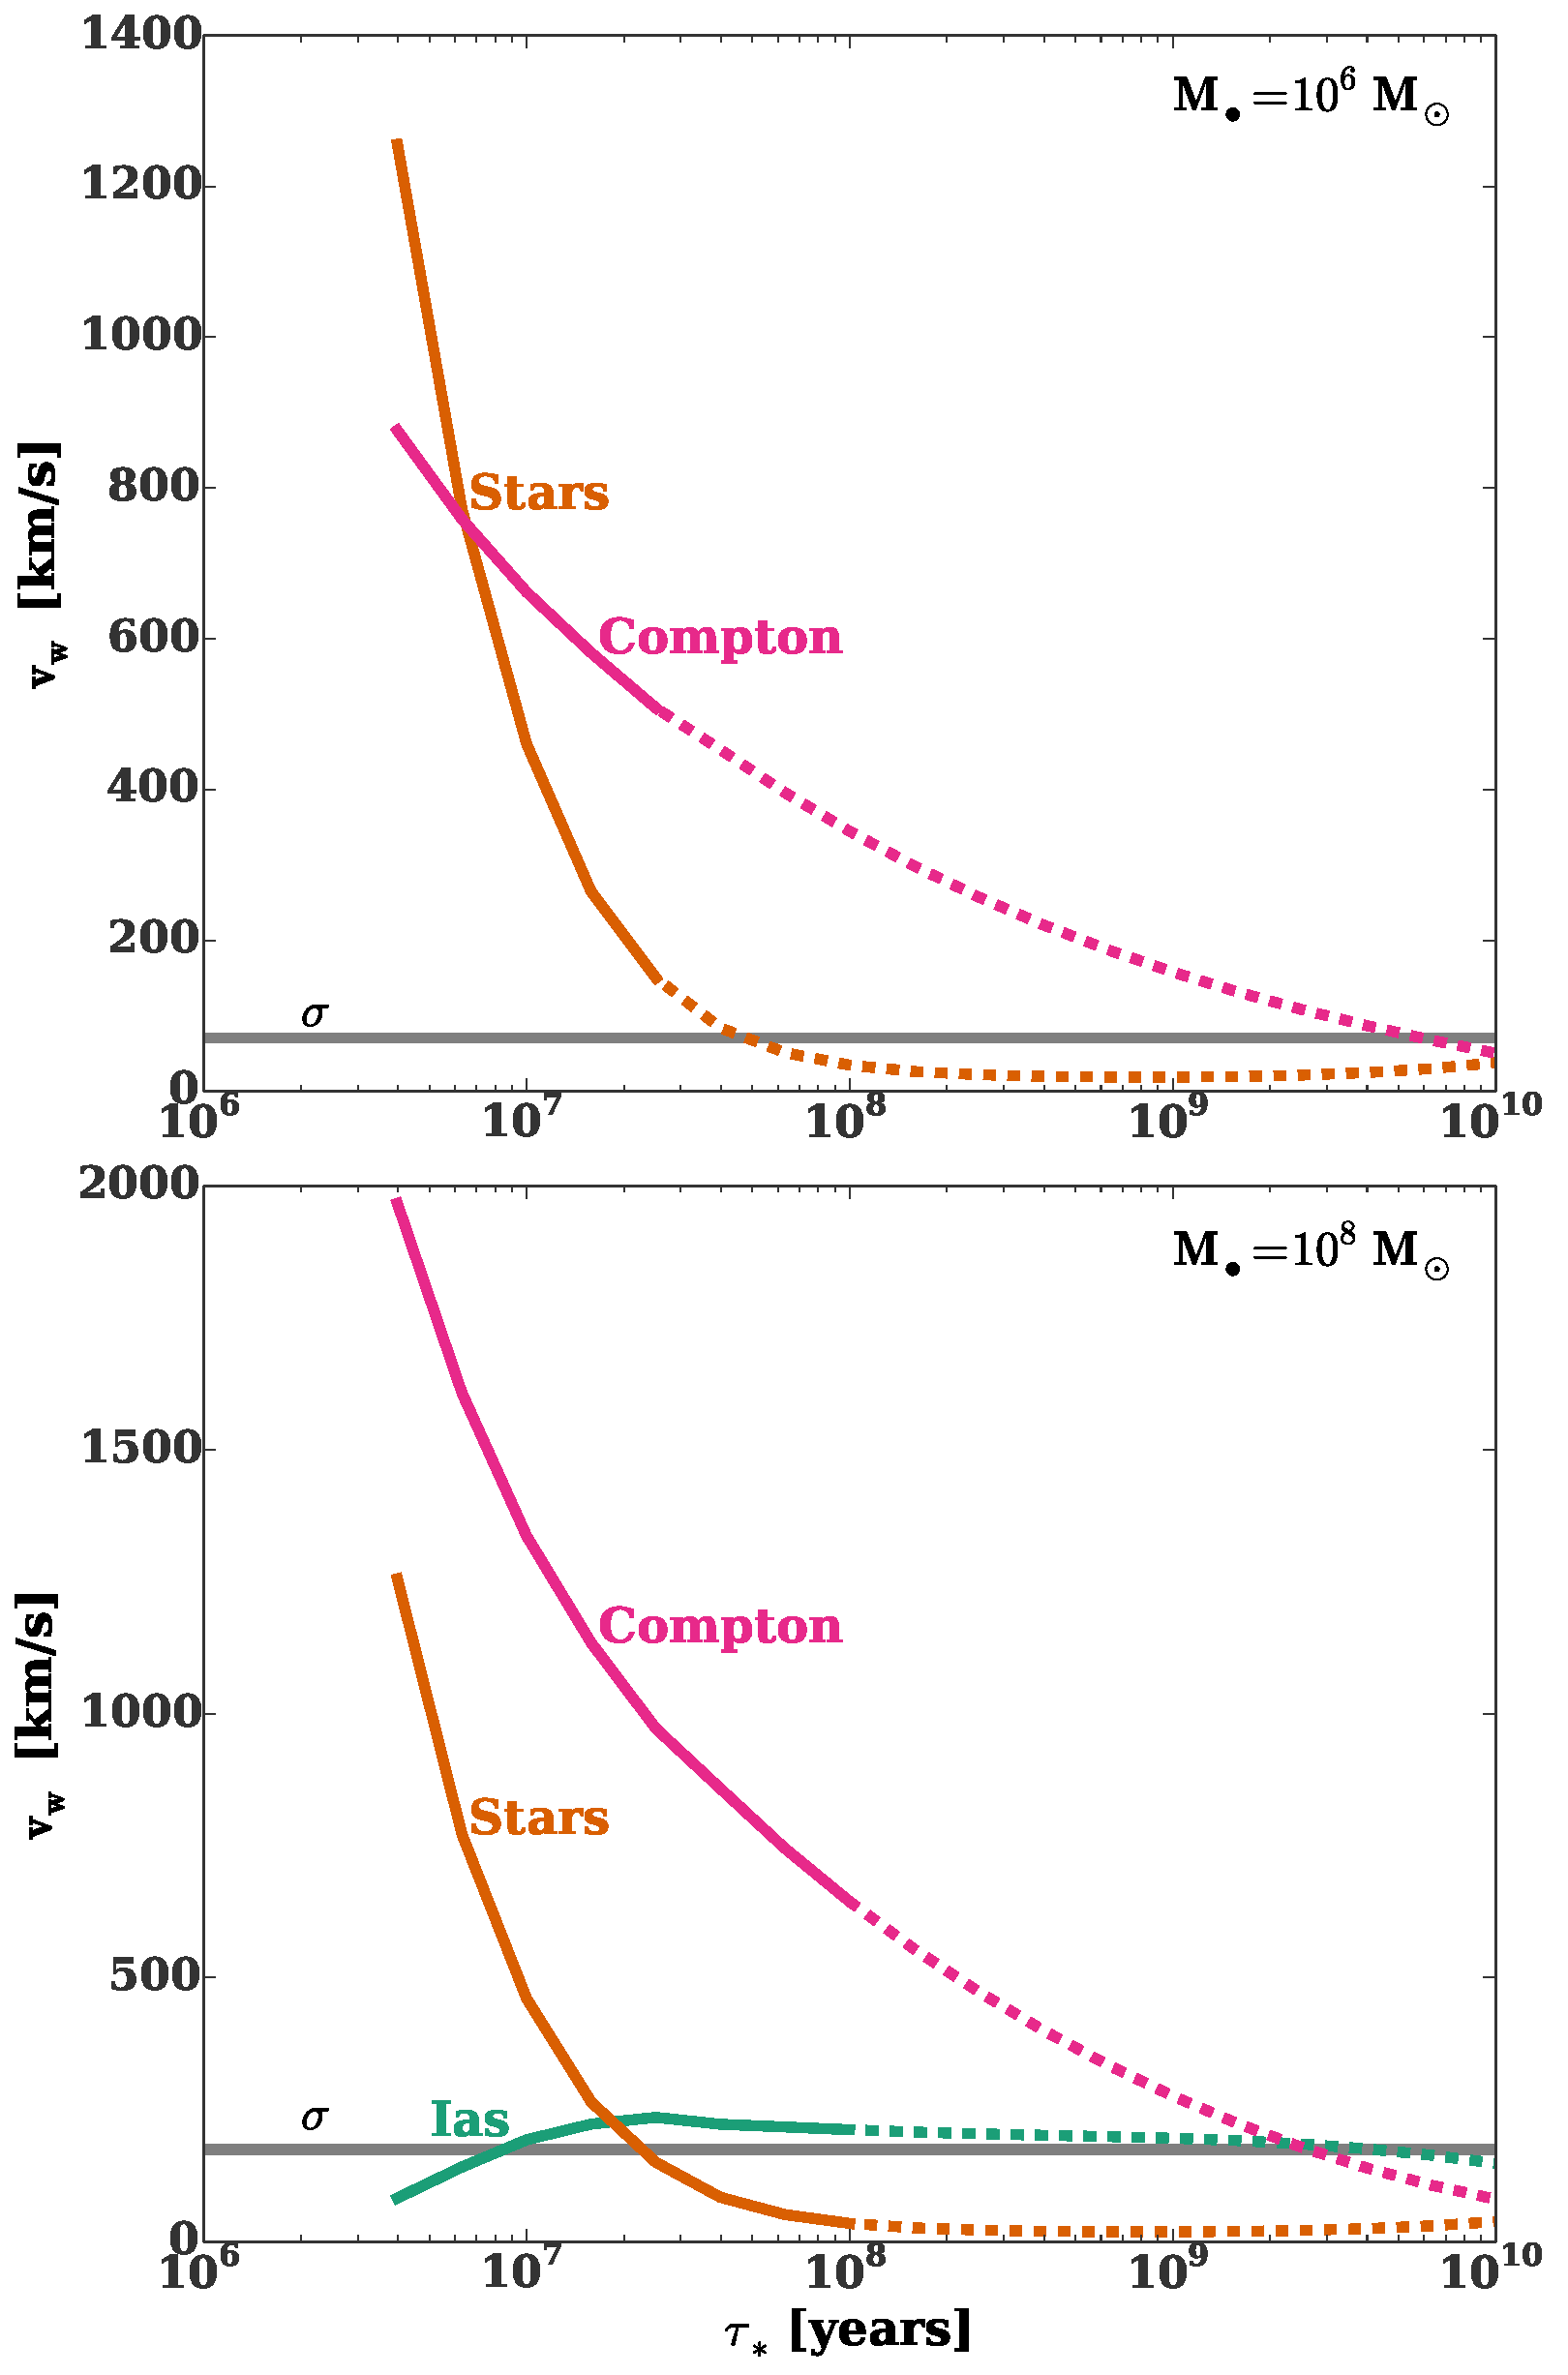
\includegraphics[width=\columnwidth]{vwSourcesImp.pdf}
\caption{\label{fig:vwSourcesImp} Different sources contributing to the gas heating rate in galactic nuclei at time $\tau_{\star}$ after a single burst of star formation.  Top and bottom panels show cases for black hole masses of $\Mbh=10^6 \Msun$ and $\Mbh= 10^8 \Msun$, respectively.  Solid and dashed lines show the ranges of $\tau_{\star}$ for which the accretion flow is thermally stable and unstable, respectively, according to the ratio of $\dot{q}_{\rm heat}/|\dot{q}_{\rm rad}|$ near the stagnation radius (eq.~[\ref{eq:cooling3}]).   Also shown with horizontal gray lines are the velocity dispersions according to $\Mbh-\sigma$ \citep{McConnellMa+:2011a}.}
\end{figure}


\begin{figure}
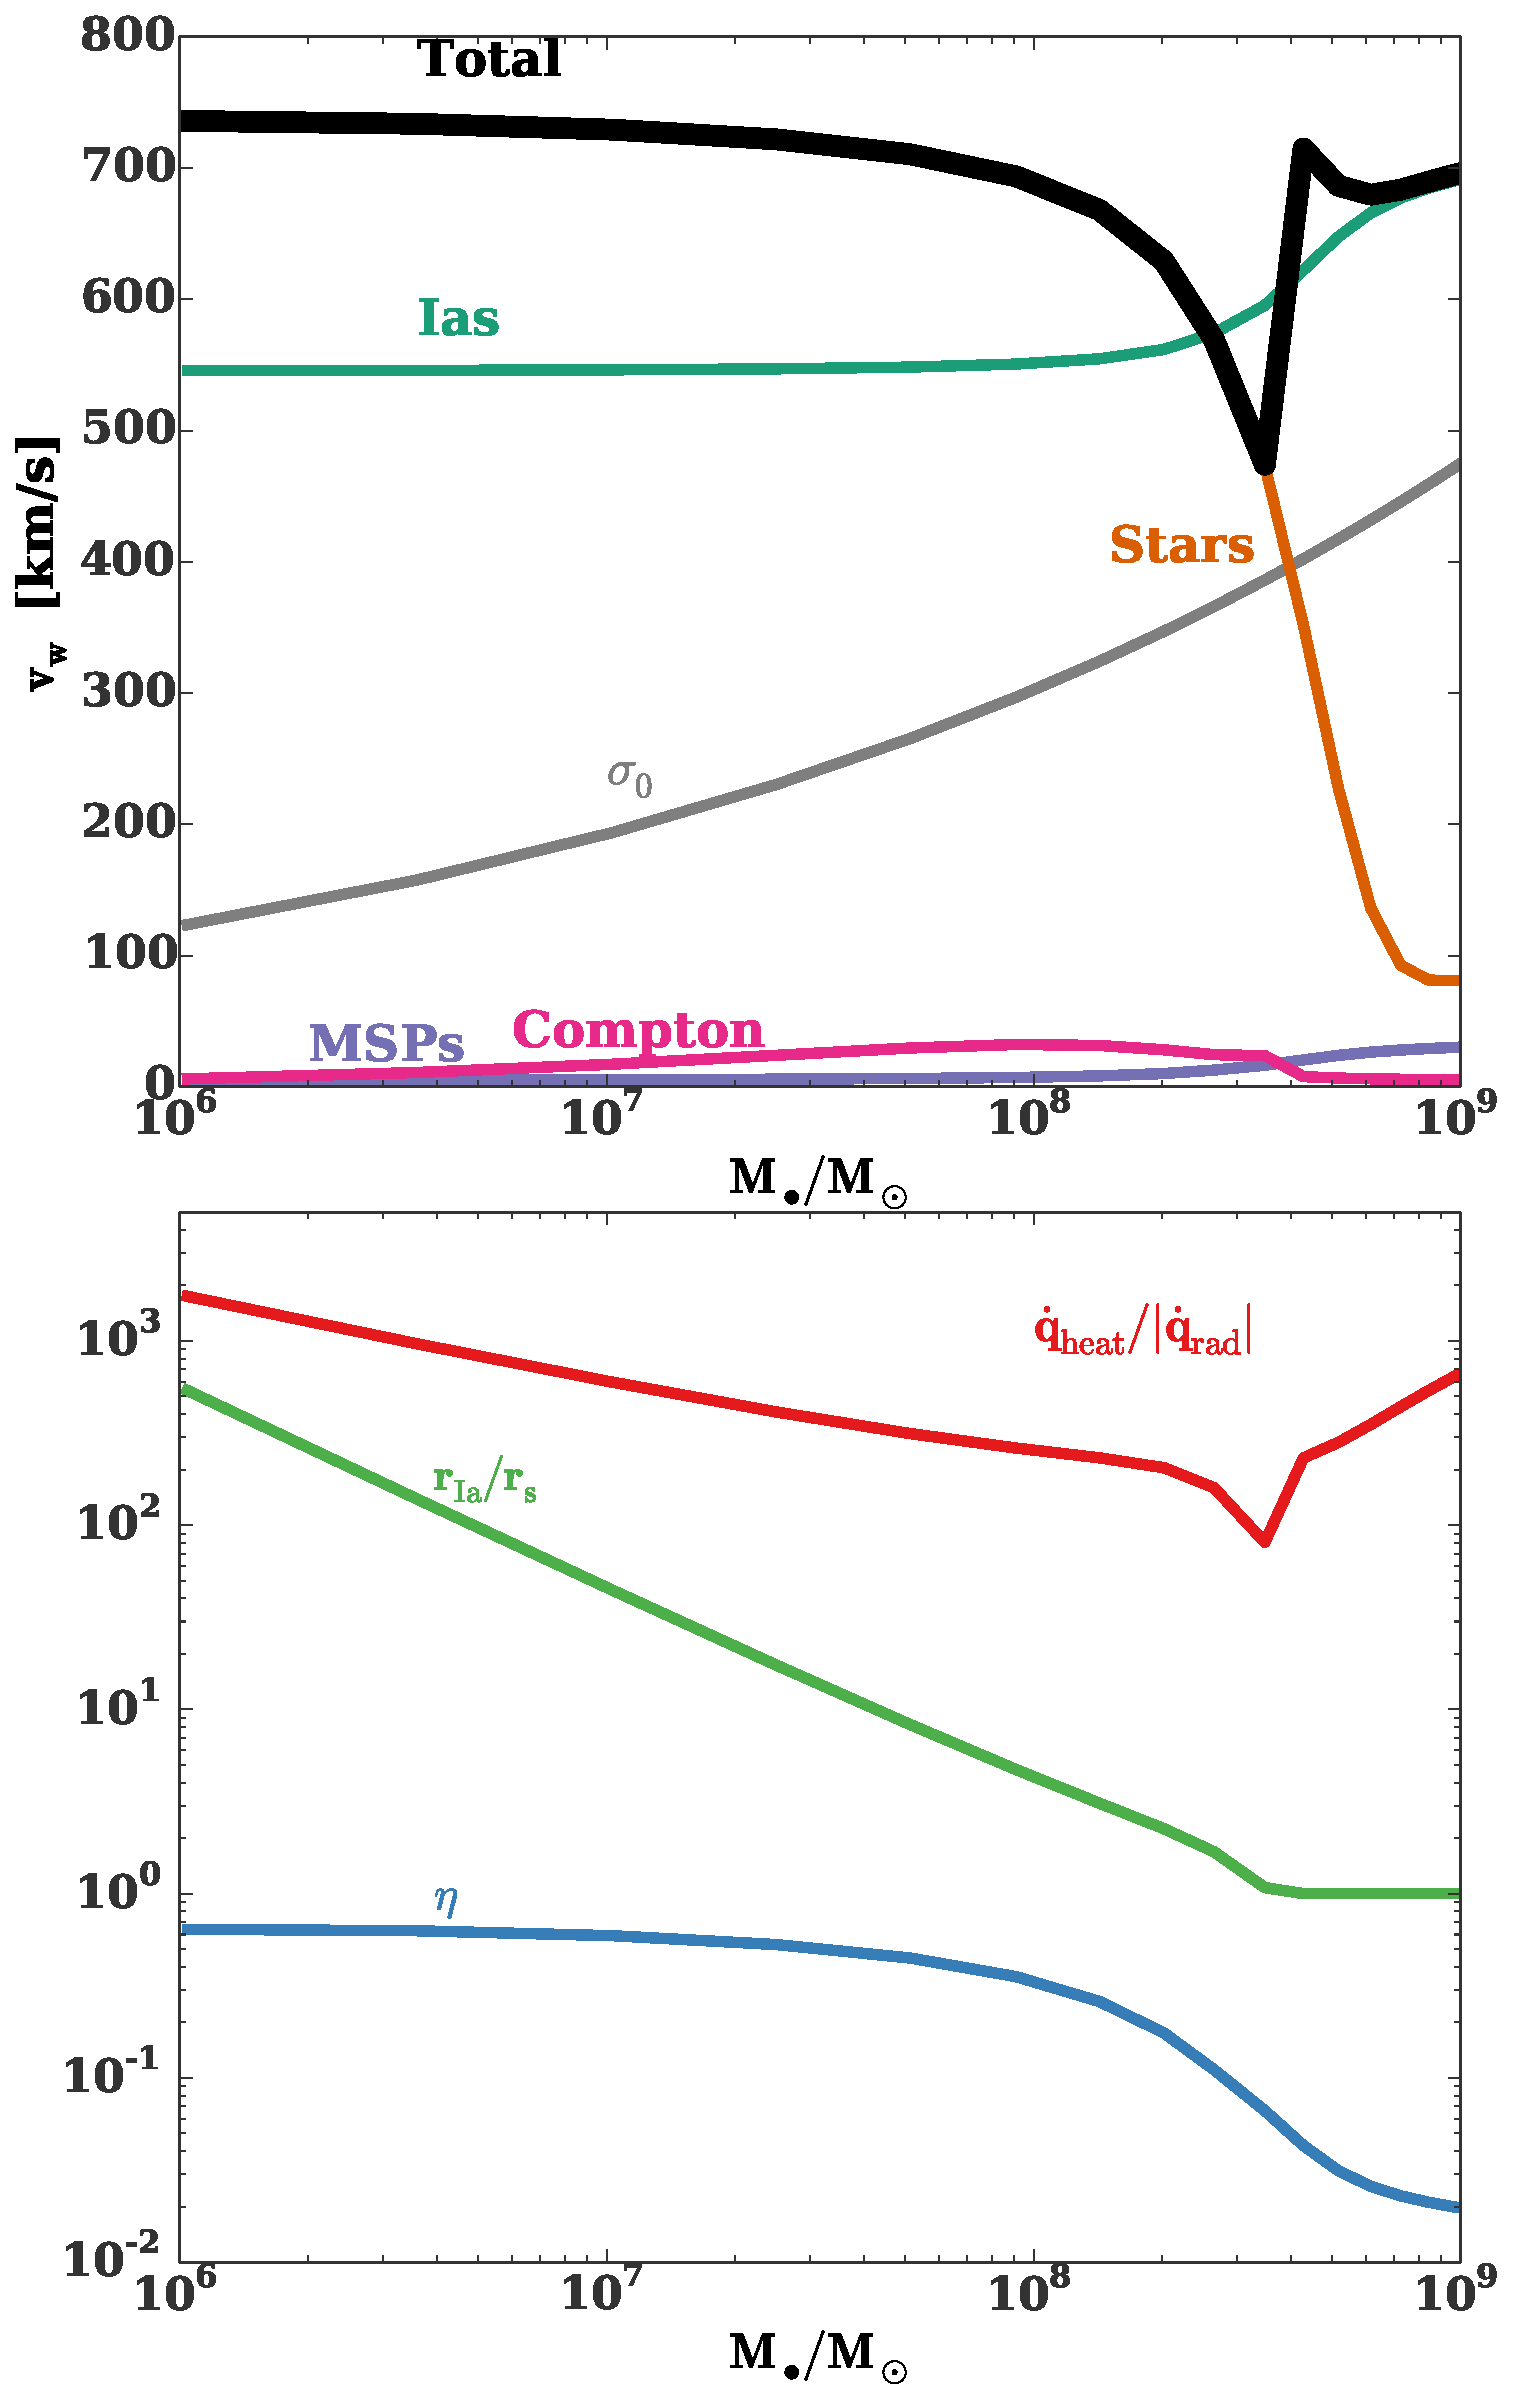
\includegraphics[width=\columnwidth]{vwSources.pdf}
\caption{\label{fig:vwSources} {\it Top Panel:} Sources contributing
  to the total heating rate of the CNM, $\vwO$ ({\it black}),
  including stellar wind heating ({\it orange}), Ia supernovae ({\it
    green}), millisecond pulsars ({\it blue}), and compton heating
  ({\it pink}).  Each heating source varies with black hole mass
  $\Mbh$ calculated for average star formation histories from
  \citet{MosterNaab+:2013a} (see Appendix~\ref{app:windheat} for
  details).  {\it Middle Panel:} The ratio of the total heating rate
  ($\dot{q}_{\rm heat} \propto v_{w}^{2}$) from the top panel to the
  radiating cooling rate ($|\dot{q}_{\rm rad}|$) at the stagnation
  radius. {\it Bottom panel} Parameter $\eta$ characterizing stellar
  mass loss rate (eq.~[\ref{eq:q}]) as a function of black hole mass
  $\Mbh$, calculated for average star formation histories from and the
  ratio of Ia radius to stagnation radius as a function of $\Mbh$.}
  %The Ia radius calculated from equation~\eqref{eq:rIa} based on
  %convolving the average star formation histories with the SN Ia DTD.
  %The stagnation radius is calculated from \eqref{eq:stag_simple}
  %using the total heating rate for each $\Mbh$ shown in the top panel
  %assuming a cusp galaxy ($\Gamma=0.8$).}
\end{figure}


% \begin{figure}
% 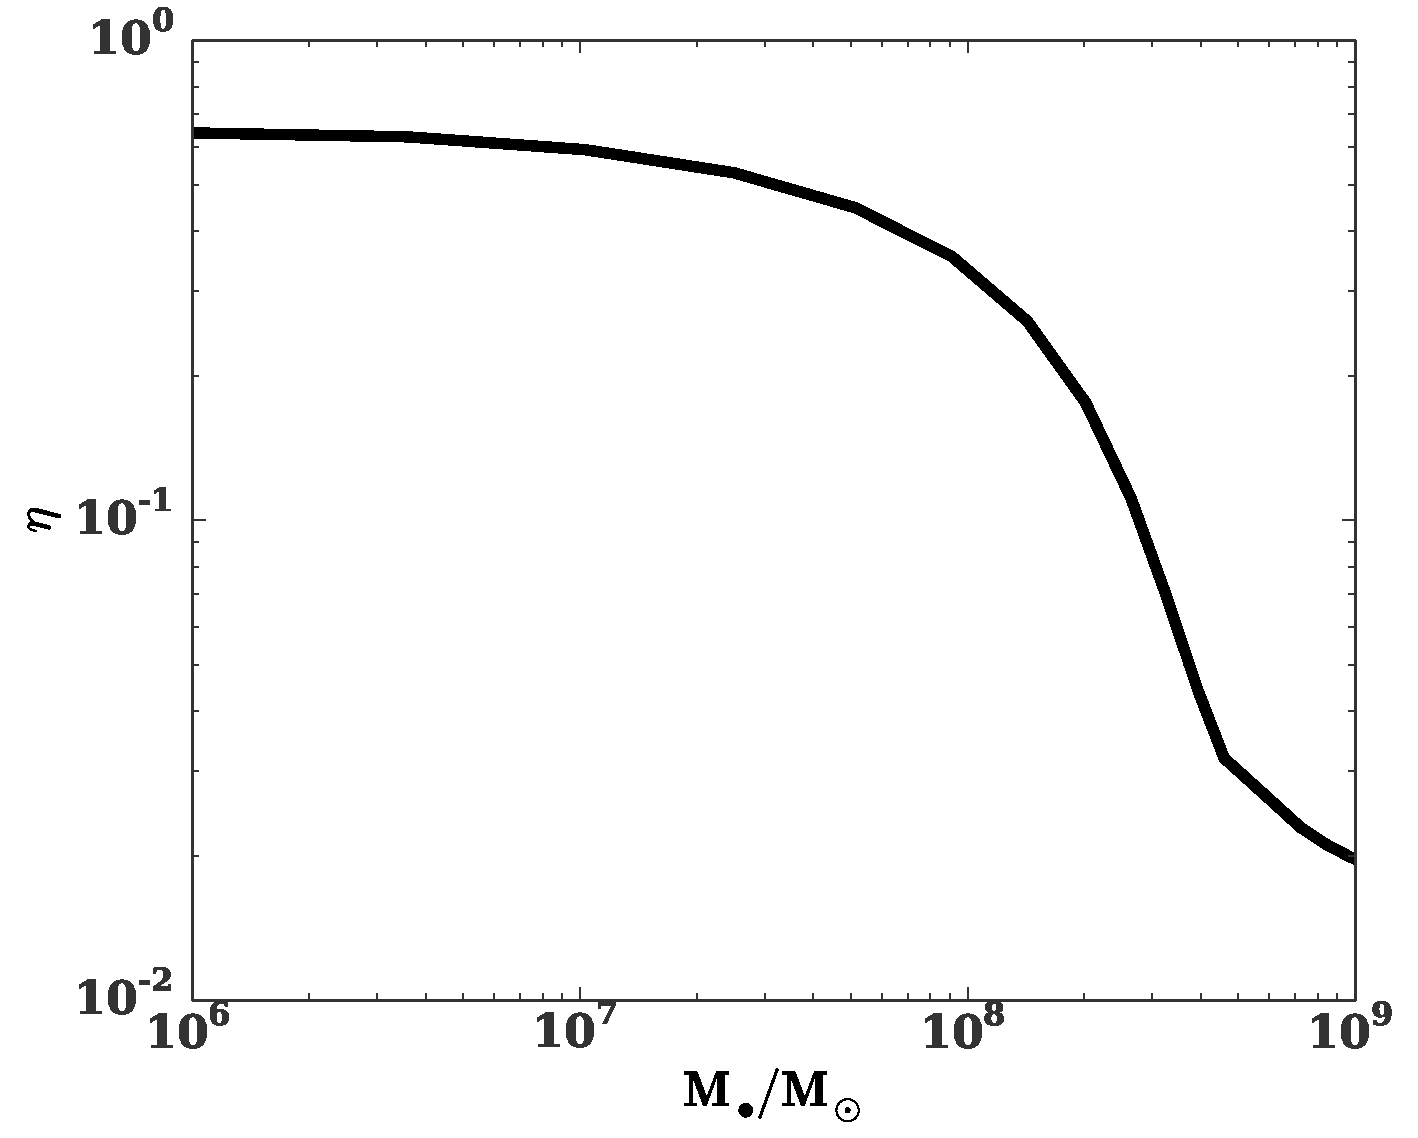
\includegraphics[width=\columnwidth]{eta.pdf}
% 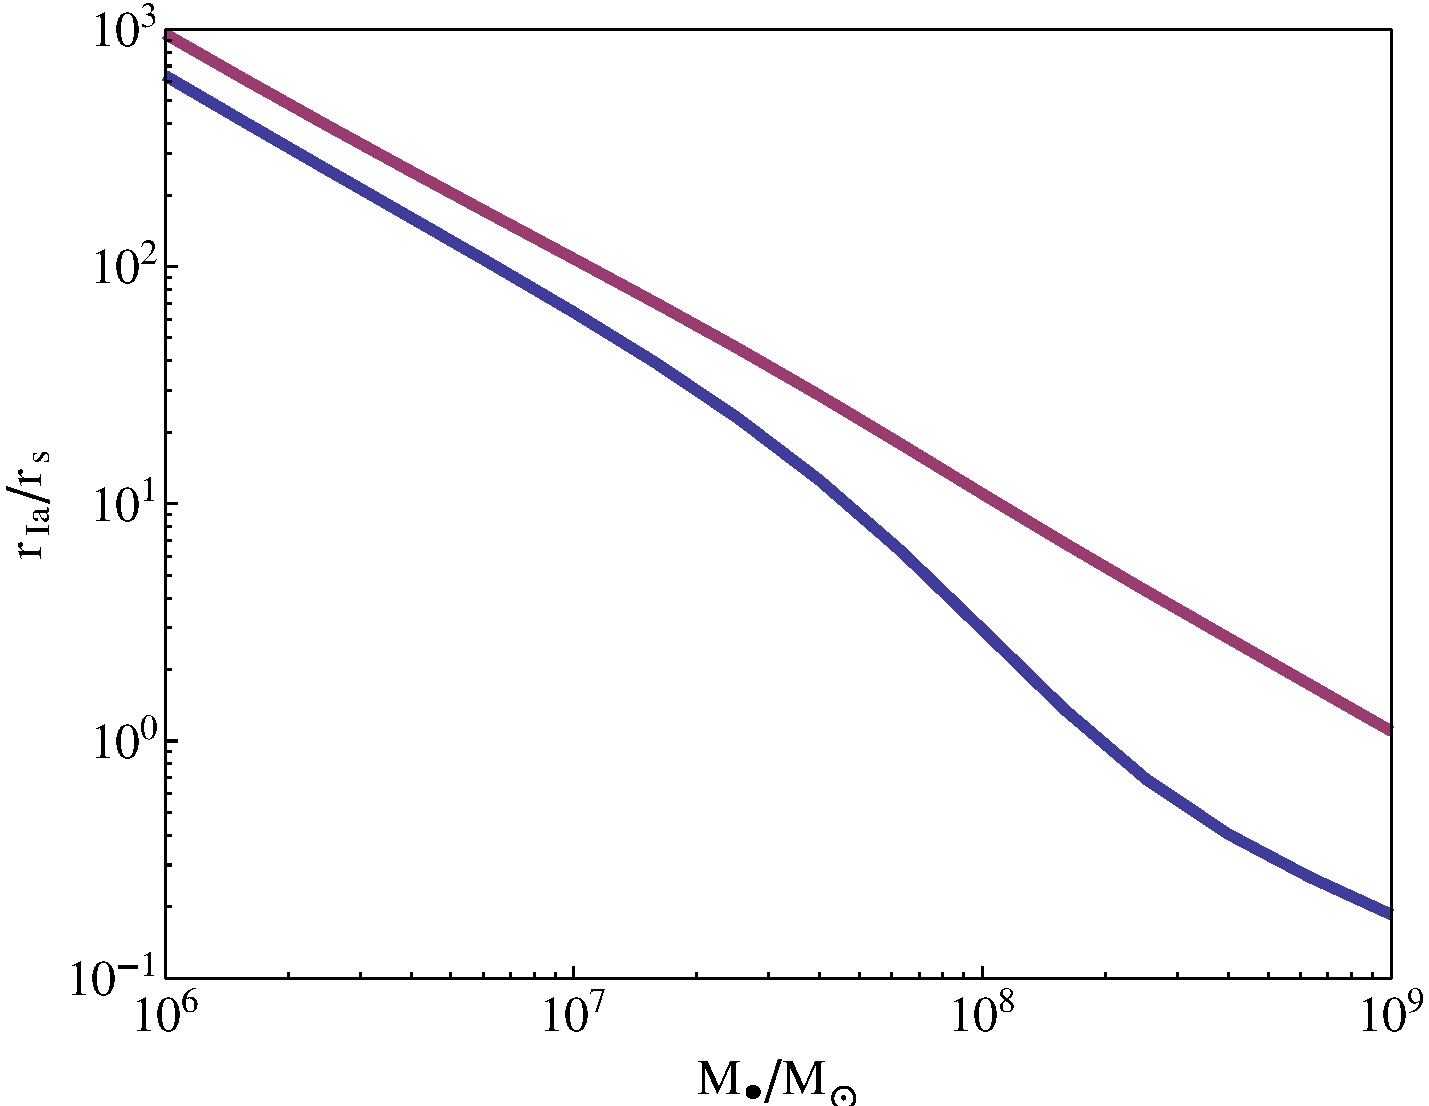
\includegraphics[width=\columnwidth]{rs_rIa.pdf}
% \caption{\label{fig:eta} {\it Top panel:} Parameter $\eta$
%   characterizing stellar mass loss rate (eq.~[\ref{eq:q}]) as a
%   function of black hole mass $\Mbh$, calculated for average star
%   formation histories from \citet{MosterNaab+:2013a} (see
%   Appendix~\ref{app:windheat} for details).  {\it Bottom panel:} Ratio
%   of Ia radius to stagnation radius as a function of $\Mbh$.  The Ia
%   radius calculated from equation~\eqref{eq:rIa} based on convolving
%   the average star formation histories with the SN Ia DTD.  The
%   stagnation radius is calculated from \eqref{eq:stag_simple} using
%   the total heating rate for each $\Mbh$ shown in the top panel. }
% \end{figure}



\subsection{Combined Heating Rate} 
\label{sec:combined}


The total gas heating rate, 
\begin{equation}
\vwO = \sqrt{(v_{w}^{\star})^{2} + (v_{w}^{\rm MSP})^{2} + (v_{w}^{\rm Ia})^{2} + (v_{w}^{\bullet})^{2}},
\label{eq:vtot}
\end{equation}
includes contributions from stellar winds, supernovae, pulsars, and radiative SMBH feedback.  The strength of each heating source depends explicitly on the SMBH mass and the stellar population in the galactic nuclear region.  The latter could best be described by a single star burst formation in the past, or by a more continuous star formation history that itself varies systematically with the galaxy mass and hence $\Mbh$.

\subsubsection{Single Starburst}

Figure~\ref{fig:vwSourcesImp} shows the contributions of various heating sources as a function of time $\tau_{\star}$ after a burst of star formation for black holes of mass $\Mbh = 10^{6} \Msun$ (top panel) and $\Mbh = 10^{8} \Msun$ (bottom panel). The heating and mass input parameters due to stellar winds, $v_{w}^{\star}(\tau_{\star})$ and $\eta(\tau_{\star})$, are calculated as described in Appendix~\ref{app:windheat} (Fig.~\ref{fig:vwImp}).  The heating from SN Ia ($v_{w}^{\rm Ia}$) and Compton heating ($v_{\rm w}^{\rm C}$) are calculated from equations~\eqref{eq:vIa} and~\eqref{eq:vC} respectively, also making use of $\eta(\tau_{\star})$ from stellar winds.  SN Ia heating depends also on a convolution of the DTD (eq. [\ref{eq:DTD}]) and the star formation history, which reduces to the DTD itself for a single star burst.  We crudely account for the expected suppression of SN Ia heating resulting from its non-steady nature by attenuating $v_{w}^{\rm Ia}$ by a factor $e^{-\rs/\rIa}$, where $r_{\rm Ia}$ is the radius exterior to which the time between subsequent supernovae exceeds the local dynamical time (eq.~[\ref{eq:rIa}]).  Finally, note that $v_{\rm w}^{\rm C}$ and $v_{\rm w}^{\rm Ia}$ also depend on the total heating rate (eq.~[\ref{eq:vtot}]), requiring us to simultaneously solve a series of implicit equations to determine each heating rate.  Heating from MSPs is found to be negligibly small for fiducial parameters and hence is not shown, while kinetic feedback is neglected given its uncertain efficiency ($\S\ref{sec:kinetic}$).  

For low-mass black holes, stellar winds are the most important source of heating on
timescales of less than a few tens of millions of years.  Compton
heating comes to dominate at later times due to the higher accretion
rates that accompany the overall decrease in the heating rate, coupled
with the persistently high mass loss rates and gas densities associated with a relatively young
stellar population.  Compton heating dominates at all epochs for
higher mass black holes, with stellar winds and Ia SN competing for
the most significant non-AGN heating source.  As the total heating
rate declines with time, after some point the flow becomes thermally
unstable according to the criterion $(\dot{q}_{\rm heat}/|\dot{q}_{\rm
  rad}|)_{r_{s}} \lesssim 1$ (eq.~[\ref{eq:cooling3}]), as shown by
dashed lines in Fig.~\ref{fig:vwSourcesImp}.  The thermal stability is
calculated neglecting Compton heating because the latter may not be
capable of truly stabilizing the flow given its inability to respond
instantaneously to local changes in the properties of the gas.
Thermally unstable flow is seen to be the norm in the single starburst
case, except at very early times, $\tau_{\star} \lesssim 1-3 \times
10^7$ yr.

\subsubsection{Continuous Star Formation History}
A single burst of star formation does not describe the typical star
formation history of most galaxies.  Qualitatively, smaller galaxies
will on average have more recent star formation, resulting in
energetic young stellar winds and supernovae which dominate the gas
heating budget.  Massive galaxies, on the other hand, will on average
possess older stellar populations, with their heating rates dominated
by SN Ia (on large radial scales) and SMBH feedback.  We estimate the
average value of $\vwO$ as a function of SMBH mass for each heating
source by calculating its value using the average cosmic star
formation histories of \citet{MosterNaab+:2013a}.  Appendix
\ref{app:windheat} describes how the average star formation history is
used to determine the stellar wind heating $v_{\rm w}^{\star}$ and
mass return parameter $\eta$ as a function of $M_{\bullet}$
(Fig.~\ref{fig:vwSources}; top panel).  Star formation histories are also
convolved with the Ia DTD distribution to determine the SN Ia heating.

Figure~\ref{fig:vwSources} shows $\vwO(M_{\bullet})$ from each heating
source (stars, MSPs, SNe Ia, and black hole feedback) calculated for
the average star formation history of galaxies containing a given
black hole mass.  Again, Ia heating is suppressed in low mass galaxies
because the Ia radius exceeds the nominal stagnation radius (bottom
panel).  MSP heating is again found to be negligible for all black
hole masses.  The younger stellar populations characterizing galaxies
with $\Mbh\lsim 5\times 10^{8} \Msun$ are dominated by stellar wind
and Ia heating, with $v_{w}^{\star} \sim 1000$ km s$^{-1}$ and
$v_w^{\rm Ia} \sim 500$ km s$^{-1}$, respectively.  Only for the most
massive galaxies, with $\Mbh\gsim 5\times 10^{8} \Msun$, does the lack
of young stellar populations significantly reduce the role of stellar
wind
heating.  %Solid and dashed lines again show black hole masses for which the flow is thermally stable and thermally unstable, respectively, with $(\dot{q}_{\rm heat}/|\dot{q}_{\rm rad}|)_{r_{s}}$ as a function of $M_{\bullet}$ shown in the bottom panel.
Strikingly, {\it we find that galactic nuclei experiencing the same
  average star formation history as their host galaxies produce
  thermally stable flows across almost all black hole masses}.  One exception may occur for the highest mass black holes, for which the total heating velocity is comparable to the stellar velocity dispersion and thermal stability for the average star formation history is marginal ($\S\ref{sec:mdot}$).
{\bf AG: I wouldn't put too much stock in this since for higher masses
vw is comparable to sigma, and thus rs should run away to large
radii. This is especially true for core galaxies.}

Realistic variations (``burstiness") in the star formation history
will often result in lower heating rates.  Figure \ref{fig:NickPlot2}
shows the heating rate as a function of average black hole mass for
non-fiducial cases in which the current ($z = 0$) star formation is
suppressed by a factor $\zeta$ from its average $z = 0$ value, for a
characteristic timescale $t_{\rm scale}$ (for details, see Appendix
\ref{app:windheat}).  For $t_{\rm scale} \lesssim 10^{7}$ yr, we see
that $v_{\rm w}^{\star}$ is reduced by at most a factor of $\approx 2$
from its average value, even for huge drops in the star formation rate
($\zeta \sim 10^{-3}$).  However, burstiness in the star formation
history over longer timescales can suppress heating more
significantly.  When $t_{\rm scale} \gtrsim 10^8~{\rm yr}$, $v_{\rm
  w}^\star$ becomes very sensitive to $\zeta$: at $\zeta=0.1$, $v_{\rm
  w}^\star \approx 500~{\rm km~s}^{-1}$ in most galaxies, but for
smaller $\zeta$, $v_{\rm w}^\star \approx 200~{\rm km~s}^{-1}$ (an
exception to this is in galactic nuclei with $M_\bullet \gtrsim
5\times 10^8~M_\odot$, where heating is stabilized by SN Ia).  Our use
of average cosmic star formation histories is appropriate provided
local variations are either on short timescales ($t_{\rm scale}
\lesssim 10^7~{\rm yr}$), or limited in magnitude ($\zeta \gtrsim
0.1$).  If both of these conditions are violated, then the effective
heating rates for all but the most massive galaxies (where Ia
explosions dominate) will fall by a factor $\approx 5$ from our
fiducial volumetric averages, taken from \citet{MosterNaab+:2013a}.


\section{Implications and Discussion}
\label{sec:discussion}

\subsection{Black Hole Accretion Rates}
\label{sec:mdot}

Figure \ref{fig:vwSources} shows that the heating associated with the
average star formation history of a galaxy is approximately constant
with SMBH mass, except for the largest black holes with $M_{\bullet}
\gtrsim 5\times 10^{8}M_{\odot}$.  For a fixed wind heating parameter,
the Eddington ratio $\dot{M}/\dot{M}_{\rm edd}$ increases $\propto
M_{\bullet}^{0.5(0.8)}$ for core(cusp) galaxies, respectively
(Fig.~\ref{fig:mdot_mass}; eq.~[\ref{eq:eddr_analytic}]).

Figure \ref{fig:bh_growth} (top panel) shows with solid lines the
accretion rate as a function of black hole mass for the average star
formation heating, calculated from equation (\ref{eq:eddr_analytic})
using our results for the total wind heating
(Fig.~\ref{fig:mdot_mass}).  This average accretion rate increases
from $\dot{M} \sim 10^{-6}-10^{-5}M_{\odot}$ yr$^{-1}$ for low-mass
black holes ($M_{\bullet} \sim 10^{6}M_{\odot}$) to $\dot{M} \sim
10^{-4}M_{\odot}$ yr$^{-1}$ for $M_{\bullet} \sim 10^{9}M_{\sun}$.
These fall below the maximum thermally stable accretion rate,
$\dot{M}_{\rm TI}$ (plotted as yellow lines), except at the highest
black hole masses $\sim 10^{9}M_{\odot}$.  For these highest mass
black holes, the maximum accretion rate as set by gas blow-out from SN
Ia (green lines; eq.~[\ref{eq:eddr_Ia}]) could instead cap the
accretion rate below the thermally-unstable value, provided that the
SN Ia heating efficiency is sufficiently high that $v_{\rm w}^{\rm Ia}
\gg \sqrt{2}\sigma \sim 400$ km s$^{-1}$ (see discussion just
preceeding eq.~[\ref{eq:eddr_Ia}]).  This is only possible if the Ia
heating efficiency is higher $\epsilon_{\rm Ia} > 0.1$ than normally
assumed (\citealt{Sharma+14}) and if the galaxy is a core.  For lower mass black holes, the
maximum accretion rate set by SN Ia is significantly higher and cannot
also prevent the development of thermally unstable flows,
i.e. $\dot{M}_{\rm Ia} \gg \dot{M}_{\rm TI}$.

Shown also for comparison in Figure \ref{fig:bh_growth} (top panel) is the accretion rate onto SgrA* calculated by \citet{Quataert:2004a}, as well as the range of $\dot{M}$ for the low-luminosity AGN NGC3115 from \citealt{ShcherbakovWong+:2014a} (who find a range of accretion rates depending on the assumed model for thermal conductivity, although they do not include saturation of the conductive flux).  The SgrA* rate exceeds our estimate of $\dot{M}$ due to the average star formation history for galaxies with the same mass black hole by almost two orders of magnitude.  This discrepency can be understood by the fact that star formation in the central parsec of the Galaxy is not in steady-state: feedback is instead dominated by the stellar winds from the ring of young massive stars of mass $\sim 10^{4}M_{\odot}$ and estimated age $\sim 10$ Myr (e.g., \citealt{Schodel+07}).  Such a star formation history is better described as a `burst' of stars, for which the value of $\eta \sim 100$ at $\tau_{\star} = 10^{7}$ yr (Fig.~\ref{fig:vwImp}) is a factor of $\sim 100$ times higher than the value of $\eta \sim 1$ predicted in the average SFH case (Fig.~\ref{fig:vwSources}, bottom panel).


\begin{figure}
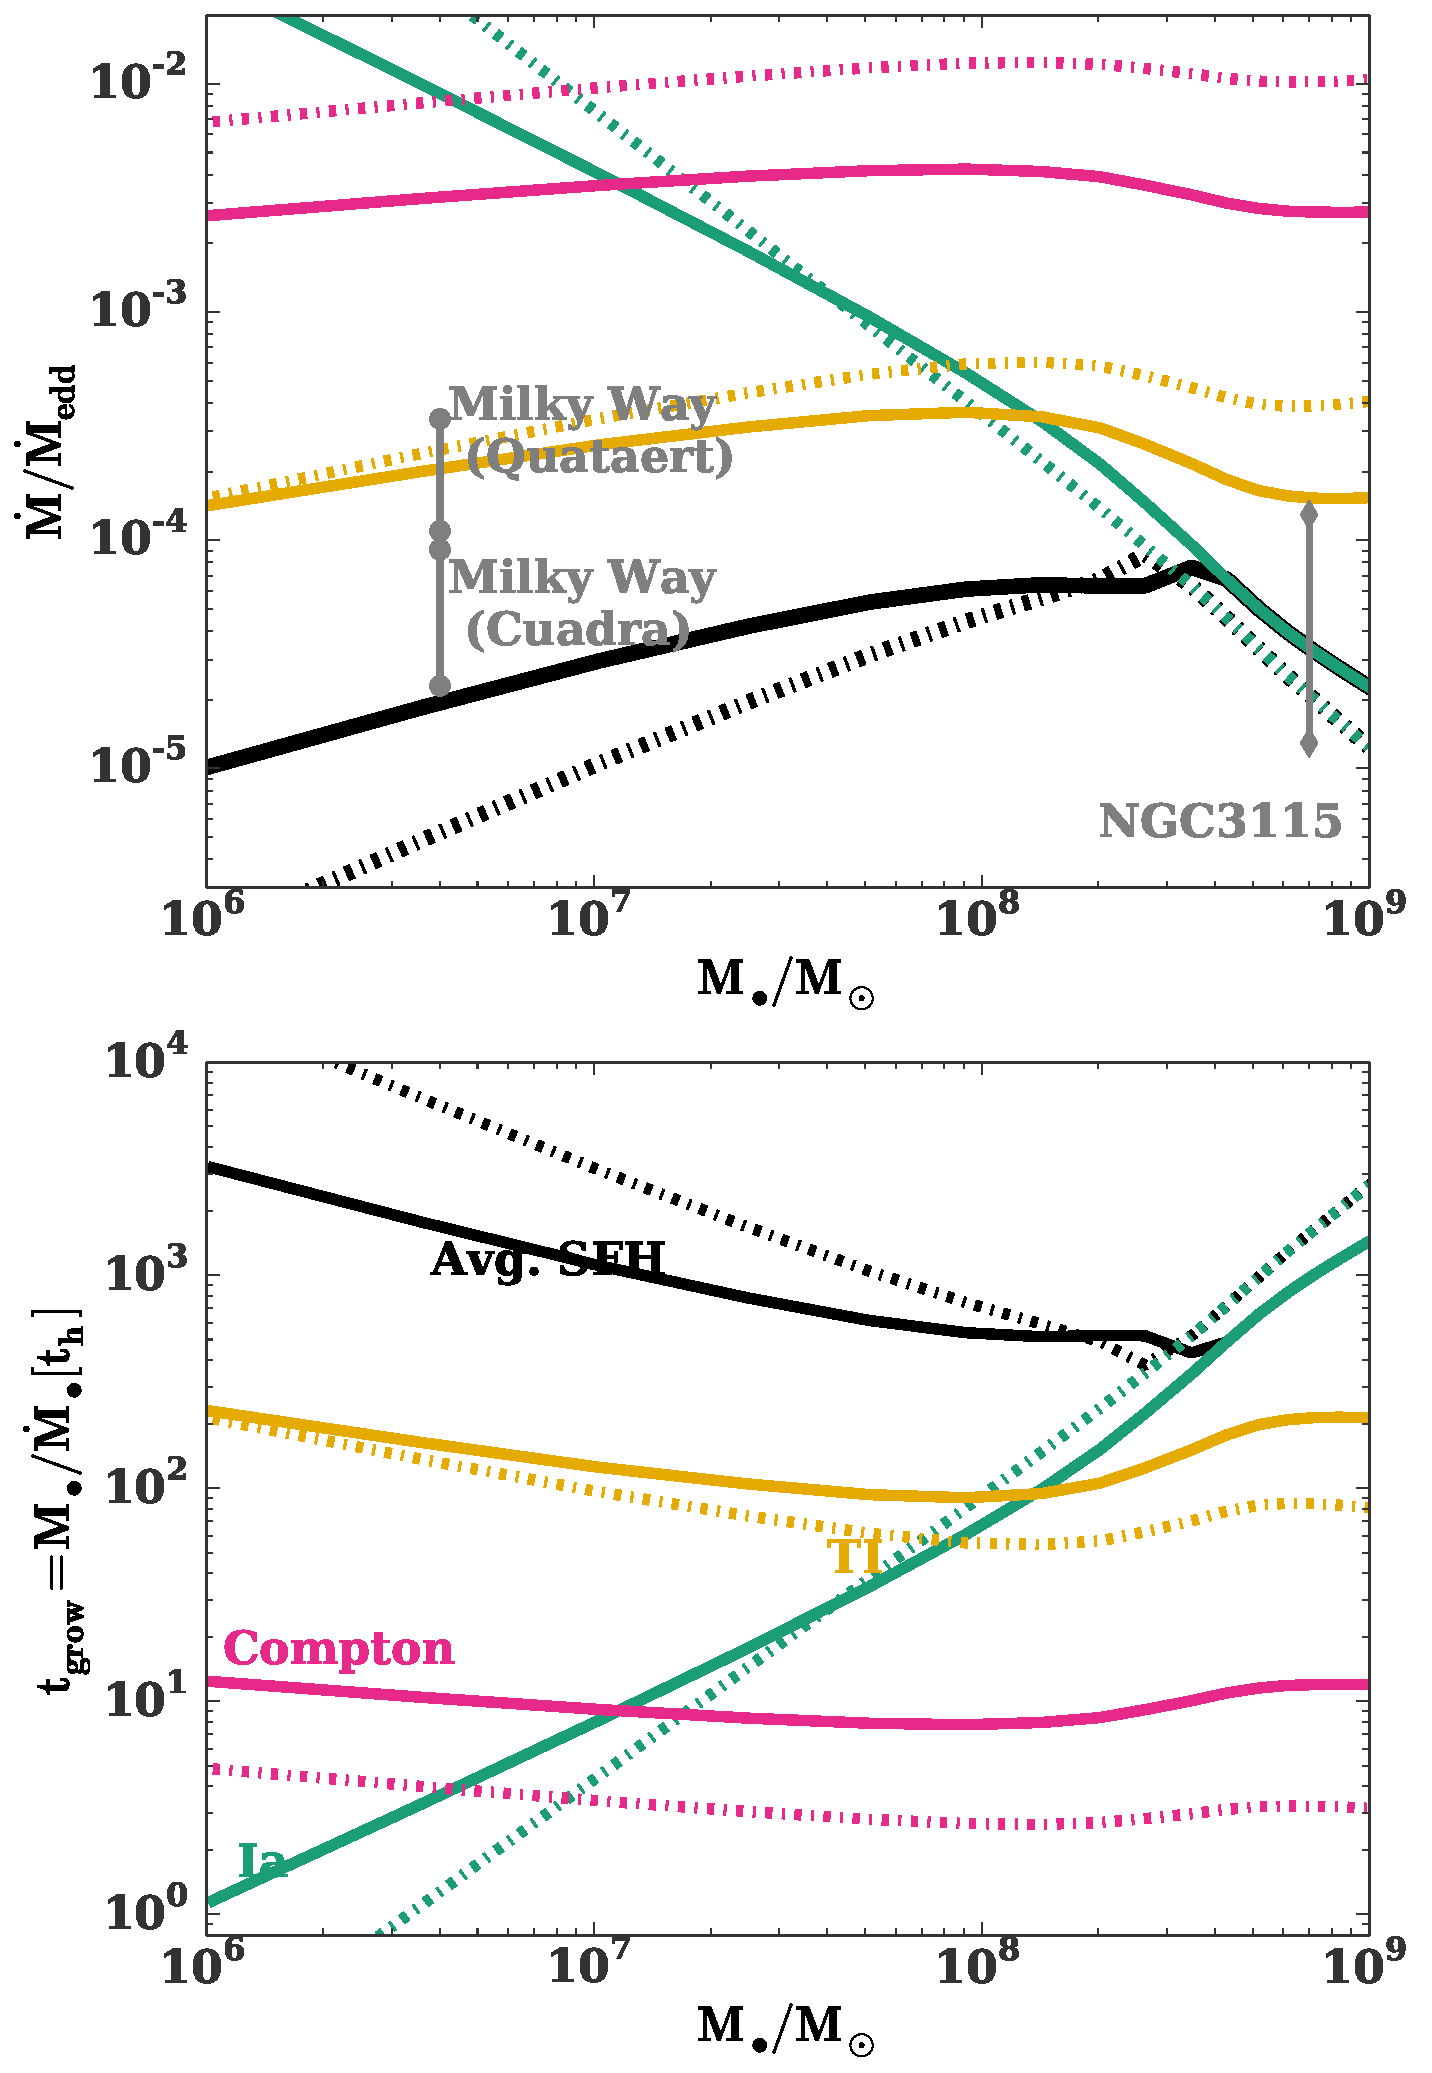
\includegraphics[width=\columnwidth]{mdot_sfr.pdf}
\caption{\label{fig:bh_growth} {\it Top panel:} Critical values of the
  black hole accretion rate $\dot{M}$ in Eddington units as a function
  of black hole mass $M_{\bullet}$, shown separately for core
  ($\Gamma=0.1$, solid lines) and cusp galaxies ($\Gamma=0.8$,
  dot-dashed lines).  Black lines show the accretion rate calculated
  from equation (\ref{eq:eddr_analytic}) using our estimate of the gas
  heating rate provided at $z = 0$ by the average star formation
  histories for each galaxy mass (Fig.~\ref{fig:vwSources}).  Green
  lines show the maximum accretion set by Ia supernovae blow-out
  (\ref{eq:eddr_Ia}).  Red lines show the accretion rate so obtained
  if Compton heating alone was acting (eq.~[\ref{eq:MdotC}]).  Yellow
  lines show the maximum accretion rate for a thermally stable flow
  near the stagnation radius (eq.~[\ref{eq:Mdotmax}]).  We also show
  Eddington ratios inferred for the galactic center from
  \citet{Quataert:2004a} (line with black circle) and for NGC3115 from
  \citet{ShcherbakovWong+:2014a} (line with black diamonds) and for
  the Swift J1644+57 event from \citet{BergerZauderer+:2012a} (line
  with black crosses) {\it Bottom panel:} Growth times $\Mbh/\Mdot$
  in units of the Hubble time $\th$ for each of the accretion rates
  shown in the top panel.}
\end{figure}

\subsection{Nuclear X-ray Luminosities}
\label{sec:Lx}

The (unresolved) core X-ray luminosities of galactic nuclei provide a
powerful diagnostic of the SMBH accretion rates and how they vary with
SMBH mass and other galaxy properties (e.g., \citealt{Ho08} and
references therein).  Figure~\ref{fig:miller} shows our predictions
for $\langle L_{X} \rangle =\epsilon_X \dot{M} c^2$ as a function of
black hole mass, where $\epsilon_{X} = \epsilon\epsilon_{\rm bol}$,
$\epsilon$ is the total radiative efficiency, and $\epsilon_{\rm bol}
\sim 0.1$ is the bolometric correction into the measured X-ray band
for low luminosity AGN (\citealt{Ho08}).  The value of $\langle L_X
\rangle$ is calculated using the average accretion for galaxies with
core ($\Gamma = 0.1$) and cusp ($\Gamma = 0.8$) stellar density
profiles, using the relationship $\Gamma = 0.3 \Mbheight^{-0.24}$ fit
to the \citet{LauerFaber+:2007a} galaxy sample.

The left panel of Figure \ref{fig:miller} is calculated assuming a
constant low value for the radiative efficiency of $\epsilon_X = 10^{-4}$,
typical of those estimated for low luminosity AGN (e.g.,
\citealt{Ho:2009a}), while the right panel luminosities are calculated
instead assuming an efficiency of $\epsilon_X= 10 \epsilon_{\rm bol}\dot{M}/\dot{M}_{\rm
  edd}$ that depends on the Eddington ratio as predicted by some
models for radiatively inefficient accretion flows
(\citealt{Narayan&Yi95}; \citealt{Narayan+98}).  Shown for comparison
are the X-ray measurements (green stars) and upper limits (gray
triangles) from the sample of early-type galaxies compiled by \citet{Miller+15}
(cf.~\citealt{Gallo+10}).  A green line shows the best power-law fit
to the X-ray luminosity from \citet{Miller+15}, given by $\langle
L_X/L_{\rm edd}\rangle \sim \Mbh^\alpha$ with $\alpha = -0.2$ (see also
\citep{Zhang+09, Pellegrini10, Gallo+10}).  Also shown are the maximum accretion rates,
respectively, for thermally stable accretion (eq.~[\ref{eq:Mdotmax}]; yellow),
as set by SN Ia blow-out (eq.~[\ref{eq:eddr_Ia}]; teal), and as allowed by
Compton heating feedback (eq.~[\ref{eq:MdotC}]; red).



\begin{figure*}
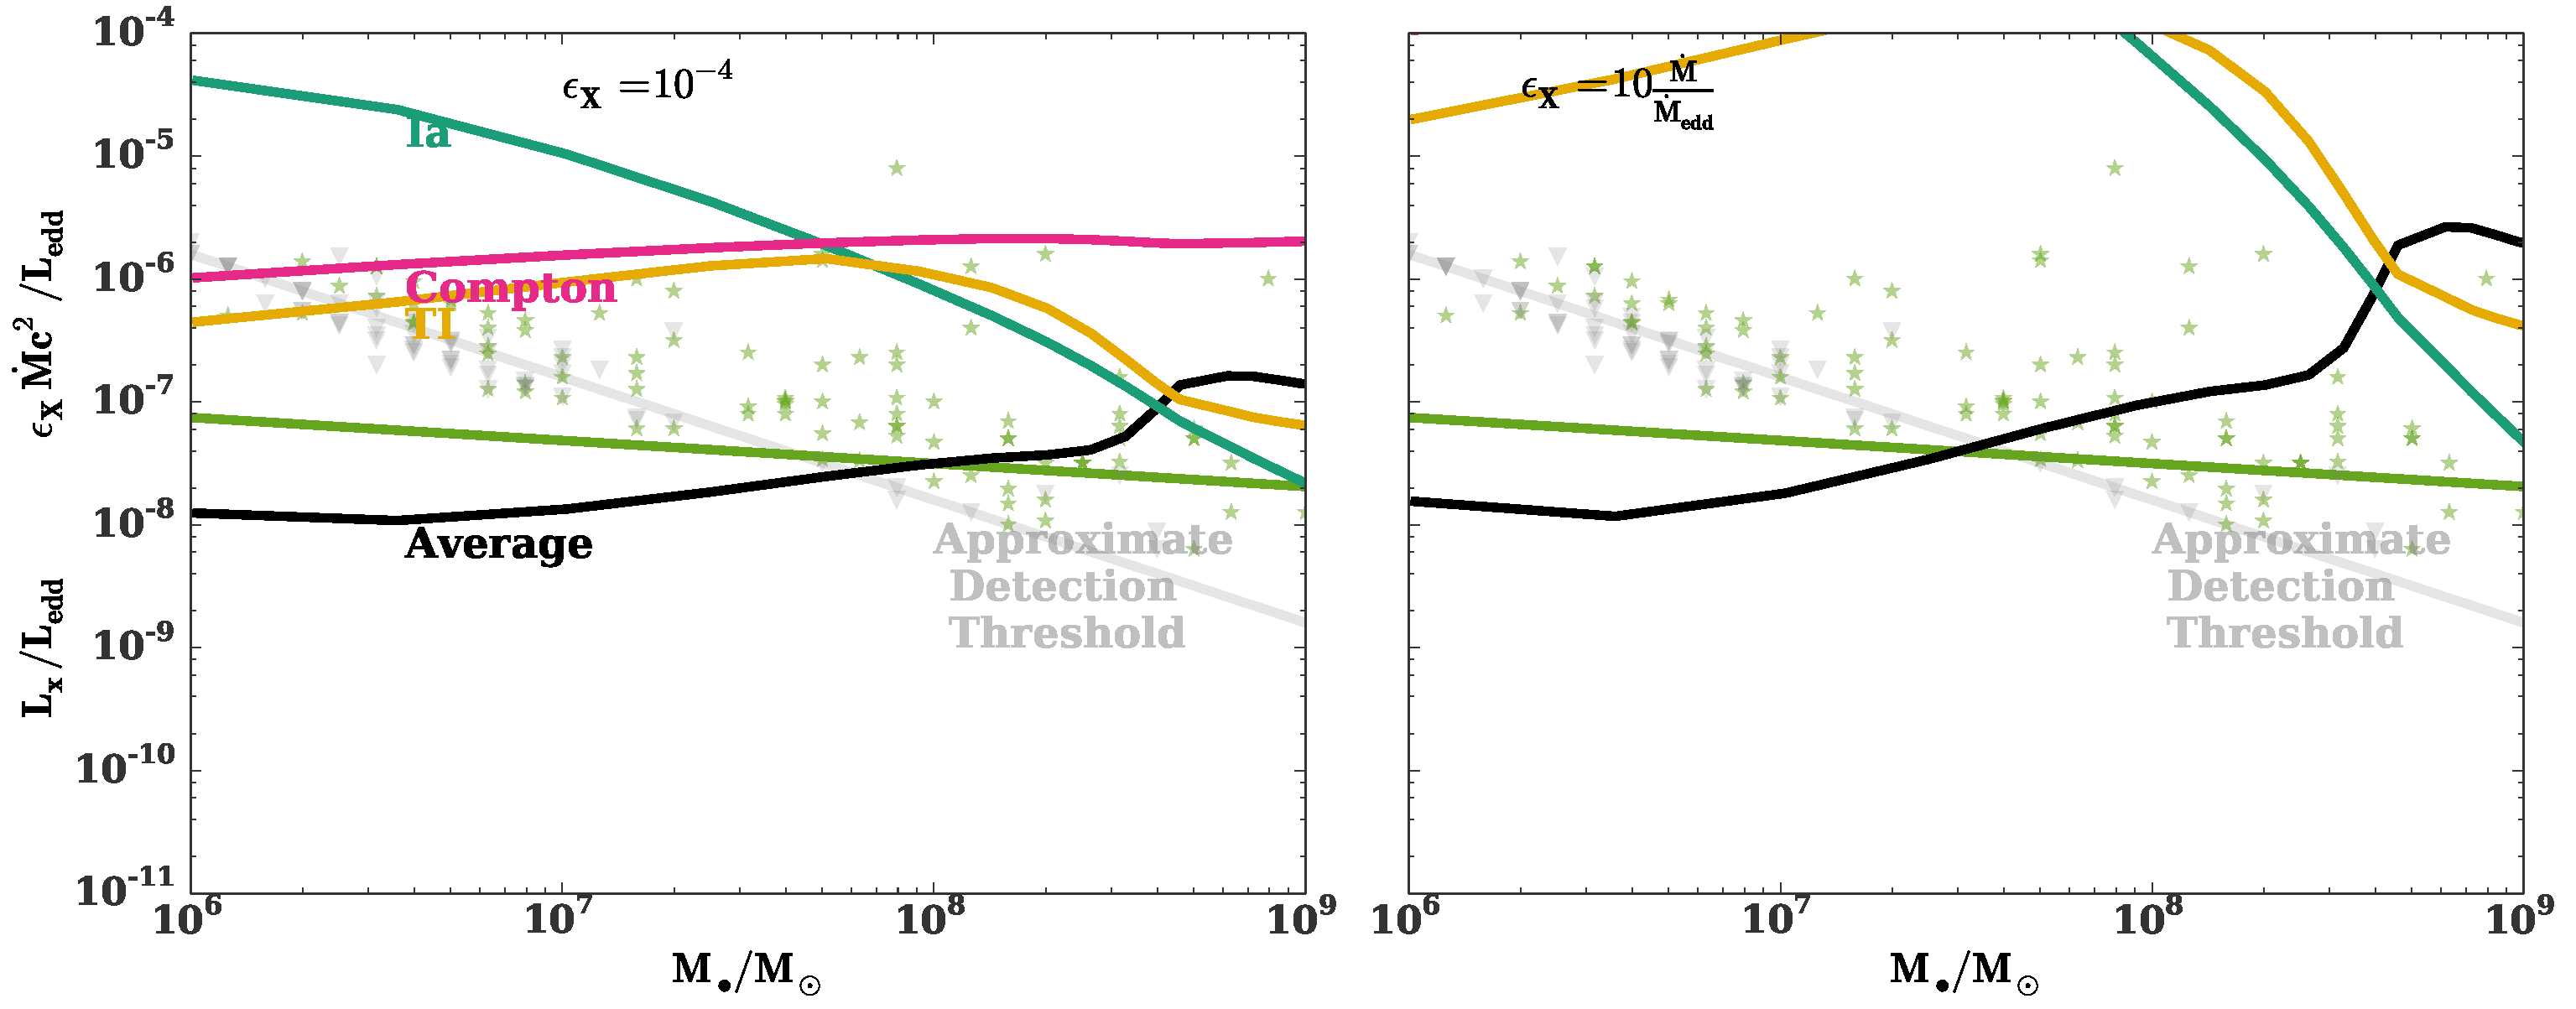
\includegraphics[width=\textwidth]{miller.pdf}
\caption{\label{fig:miller} Average (unresolved) nuclear X-ray luminosity $\langle L_X \rangle = \epsilon_X \Mdot c^2$ as a function of SMBH mass, predicted from our models for the average star formation history (Fig.~\ref{fig:bh_growth}; {\it black line}) calculated for the average Nuker power-law index $\Gamma(M_{\bullet})$ derived from the galaxy sample of \citet{LauerFaber+:2007a}.  Shown for comparison are the measurements $L_X/L_{\rm edd}$ values (red stars) and
  upper limits (red triangles) from the \citet{Miller+15} sample of early-type galaxies, with a green line showing the best power-law fit $\langle L_X/L_{\rm edd}\rangle \propto M_{\bullet}^{\alpha}$, with $\alpha = -0.2$.  The left panel shows the case of a constant radiative efficiency $\epsilon_X=10^{-4}$, while the right hand panel shows an efficiency $\epsilon_X=
  \left(\frac{\epsilon_{\rm bol}}{0.1}\right)\frac{\Mdot}{\MdotEdd}$ predicted by some models for radiatively inefficient accretion.  Also shown for comparison are the X-ray luminosities calculated using the maximum thermally-stable accretion rate ({\it orange line}), SN Ia-regulated accretion rate, and Compton-regulated accretion rate ({\it pink line}),  again calculated for the average star formation history.}
\end{figure*}

If the nuclei of elliptical galaxies are heated in a way similar to that due to the average star formation history of galaxies with
similar mass, then to first order we predict that $\langle
L_{X}/L_{\rm edd}\rangle$ should increase with black hole mass, though
only weakly for $M_{\bullet} \lesssim 3\times 10^{8}M_{\odot}$.  This
result is in tension with the observed down-sizing trend that the
average Eddington ratio is seen to decrease (albeit also weakly)
with $M_{\bullet}$.  However, one must keep in mind the enormous uncertainty in calculating the
luminosity of the accretion flow close to the black hole in a single
waveband based on the feeding rate on larger scales.  If disk outflows carry away most of the infalling mass before it reaches X-ray producing radii (e.g.~\citealt{Blandford&Begelman99}; \citealt{Li+13}), then the
angular momentum of the infalling gas might also influence the X-ray luminosity, in a way
that could depend systematically on the stellar population and hence $M_{\bullet}$.

Perhaps a more readily addressable test is whether a steady-state accretion
picture can account for the the large scatter, typically of $2-3$ orders of magnitude, in $L_{X}/L_{\rm
  edd}$ at fixed $M_{\bullet}$.  Scatter could result from at 
least three effects: (1) instric scatter in the scaling relationships ($\Mbh-\sigma$ and $\Mbh-L_{\rm
  bulge}$) used to measure $\Mbh$; (2) the strong sensitivity of the accretion rate to
the stellar wind velocity, $\dot{M}/\dot{M}_{\rm edd} \propto
v_{w}^{-3.8(-2.4)}$ for core(cusp) galaxies, respectively
(Fig.~\ref{fig:mdot_mass}; eq.~[\ref{eq:eddr_analytic}]).  When 
combined with the significant dependence of $v_w$ on stochastic
intermittency in the star formation history (Appendix
\ref{fig:NickPlot2}), this can lead to order of magnitude differences
in $\dot{M}$; (3) differences angular momentum of the infalling gas
from galaxy to galaxy, resulting in differences in the fraction of the
gas lost to outflows, $\Mbh$.  Also potentially contributing is the
order of magnitude difference, at fixed $v_w$ and $M_{\bullet}$,
between $\dot{M}$ for core and cusp galaxies
(Fig.~\ref{fig:bh_growth}).  Differences in $\dot{M}$ are augmented by
the expectation that $L_{\rm X} \propto \dot{M}^{2} $ for radiatively
inefficient flows {\bf AG: Don't forget differences in eta}. 



%Many of the upper
%limits on $L_{\rm X}$ at low $M_{\bullet}$ may in fact correspond to a
%separate ``thermally stable" population.  This possible dichotomy
%calls into question the use of simple extrapolations of power-law fits
%to the $L_{\rm X}(M_{\bullet}$) relationship to low $M_{\bullet}$ to
%constrain the occupation fraction of black holes in low mass galaxies
%(\citealt{Miller+15}).


\subsection{Steady Accretion versus Cyclic Outbursts}
\label{sec:cycle}

It is also possible that many of the galactic nuclei from the \citet{Miller+15} sample are not accreting in a steady fashion.  The efficiency assumed in the right panel of Figure \ref{fig:miller} in some ways represents a maximum value, since it does not take into suppression of the accretion rate due to disk outflows on small scales.  If the actual X-ray efficiency is lower than assumed, then many of the detections in the case of low SMBH masses, $M_{\bullet} \lesssim 10^{8}M_{\odot}$, would lie even further above above the predicted average value for stable accretion (black line).  These galaxies either experience significantly lower levels of heating than average galaxies of their mass, or that they are not accreting stably at all.  Indeed, for the lowest mass holes, $M_{\bullet} \lesssim 10^{8}M_{\odot}$, $L_{\rm X}$ nearly exceeds that predicted for the maximum thermally-stable accretion rate, $\dot{M}_{\rm TI}$ (yellow line).  It is not surprising that this sample is more likely to be thermally unstable as compared to an average galaxy with this black hole mass, because the \citet{Miller+15} sample includes only early-type galaxies with on averager older stellar populations.  

Figure \ref{fig:bh_growth} (top panel) also shows that across all black hole masses, Compton heating also cannot prevent average accretion rates which are thermally unstable, i.e. $\dot{M}_{\rm C} > \dot{M}_{\rm TI}$.  In the case of thermal instabilities, nuclear gas may undergo cyclic oscillations of rapid cooling and high accretion rates, followed by quiescent
periods once gas has been consumed and/or AGN feedback becomes effective.  Such cycles are proposed to occur on large scales and long timescales in elliptical galaxies (\citealt{Ciotti+10}), an idea possibly supported by, e.g., GALEX observations showing that a small fraction of early-type galaxies in the local universe have undergone recent ($< 1-2$ Gyr old) star formation episodes (\citealt{Donas+07}).  Similiar cyclic AGN activity have been proposed to occur on the smaller scale of the sphere of influence (e.g.~\citealt{Yuan&Li11}, \citealt{Cuarda+15}).  

If such cyclic outbursts also manifest on the properties of gas on small, parsec scales, then the large scatter in the accretion rates and hence X-ray luminosities in Fig \ref{fig:miller} could result from the wide range of inflow rates experienced over the course of a cyclic episode between instabilities and periodic nuclear outbursts (e.g.~\citealt{Ciotti+10}).  Due to their deeper potential well, we find that core galaxies are more likely to possess higher accretion rates and potentially be thermally unstable for a fixed wind heating rate than cusp galaxies (Fig.~XXX).  This could help explain why core galaxies show a wide range of nuclear radio and X-ray luminosities (suggesting cyclic accretion episodes), while cusp galaxies are confined below a threshold (e.g., \citealt{Bender+89,   Pellegrini99, Capetti&Balmaverde05}), consistent with thermally-stable, steady-state picture.

If the galaxies with measured $L_{\rm X}$ at low $M_{\bullet}$ in Fig \ref{fig:miller} represent thermally-unstable galaxies, then many of the upper limits may correspond to a separate ``thermally stable" population, for instance including SgrA*.  The possibility of a mixed population of stable versus unstable galaxies calls into question the use of simple extrapolations of power-law fits to the $L_{\rm X}(M_{\bullet}$) relationship to low $M_{\bullet}$ to constrain the occupation fraction of black holes in low mass galaxies (\citealt{Miller+15}).

%The cyclic model predicts that high $L_{X}$ nuclei should be more
%common in galaxies with younger stellar ages, a result which appears
%in tension with the finding by \citet{Pellegrini10} that galaxies with
%younger stellar populations are observed to host less X-ray luminous
%nuclei, at least for stellar ages $<3$ Gyr.  An alternative
%explanation for this observation within a thermally stable,
%steady-state accretion picture is that young stars provide higher
%stellar wind heating, reducing the mass accretion rate and hence
%nuclear X-ray luminosity.  {\bf AG Challenge: \citet{HeckmanBest:2014a}
 % find that ${\rm L_{[OIII]}}$ (a proxy for the bolometric luminosity)
  %${\rm L_{[OIII]}/M_\star}$ (a proxy for the Eddington ratio)
  %increases with decreasing 4000 $\AA$ break index (decreasing stellar
 % age) (see their Figure 14). This suggests that the accretion rate is
  %actually increasing towards younger stellar ages. At young ages
  %there actually seems to be plenty of gas around, which may be
  %obscuring the x-rays and causing an anamolously low measurement of
  %$L_X$. 
  
  %For a starburst the black hole accretion rate lags the star
  %formation rate by 200 Myr (\citet{WildHeckman+:2010a} Figure
 % 9). This could be due to SNe feed back suppressing the black hole
  %accretion rate (massive star winds do the same thing by themselves,
 % but they cannot be sustained for 200 Myr. 
%}


\subsection{Local Growth Time of SMBHs }
\label{sec:growth}

Low-mass AGN in the local universe ($M_{\bullet} \lesssim 3\times
10^{7}M_{\odot}$) are observed to be growing on a timescale comparable
to the age of the universe, while the most massive SMBHs with
$M_{\bullet} \gtrsim 10^{9}M_{\odot}$ possess local growth times which
are more than 2 orders of magnitude longer (\citealt{Heckman+04};
\citealt{Kauffmann&Heckman09}).

The bottom panel of Figure~\ref{fig:bh_growth} shows the SMBH growth
time, $t_{\rm grow} = M_{\bullet}/\dot{M}$, for each accretion rate
shown in the top panel.  For black holes accreting steadily given the
stellar wind heating associated with the average star formation
history of their galaxies, we see that $t_{\rm grow}$ exceeds the
Hubble time by 1$-$3 orders of magnitude across all black hole masses.
Steady accretion therefore cannot explain the growth of low mass black
holes, a fact which is not surprising given that approximately half of
this growth occurs in AGN radiating within 10 per cent of their
Eddington rate (\citealt{Heckman+04}).  Such high accretion rates
likely instead require an source of gas external to the nuclear
region, triggered either by galaxy mergers associated with the
hierachical growth of structure or thermal instabilities on larger,
galactic scales (e.g.~\citealt{Ciotti+10}).  In support of this, \citet{Kauffmann&Heckman09} find that the growth of low mass black holes is dominated by young stellar bulges which have a log normal
distribution of Eddington ratios peaked at $\Mdot/\MdotEdd\sim
0.01$. That this distribution is insensitive to galaxy properties suggestes that it is set by SMBH feedback instead of the nuclear gas supply.

That the growth time associated with thermally-unstable accretion
(yellow line) exceeds the Hubble time across all SMBH masses
highlights the fact that signifcant black hole growth in the local
universe cannot result from thermally-stable steady accretion of gas
lost from the surrounding stellar population studied in this paper.  Gas blow-out by SN Ia cannot prevent the growth of low-mass black holes, as indicated by the low growth times $\ll t_{\rm h}$ allowed by
Ia heating (green lines), although Ia heating could play in principle a role in capping the growth rate of $\gtrsim 10^{8}M_{\odot}$ black holes, again depending on the efficiency of Ia heating and whether the galaxy is a core or cusp.


\subsection{TDE Jets}
\label{sec:TDE}

Our results also have implications for the environments encountered by
relativistic jets from TDEs.  For low-mass SMBHs $M_{\bullet} \lesssim
10^{7}M_{\odot}$, characterizing those responsible for {\it Swift}
J1644+57 (\citealt{Bloom+11}), we predict gas densities of a $n
\sim 0.3-3$ cm$^{-3}$ on radial scales of 0.3 pc for wind heating
rates within the physically expected range $v_{\rm w} \sim 500-1000$
km s$^{-1}$ (Fig.~\ref{fig:profiles}).  These values are within the
range estimated by modeling the radio afterglow of {\it Swift}
J1644+57 (\citealt{Metzger+12}, \citealt{BergerZauderer+:2012a}).  

\citet{BergerZauderer+:2012a}  infer a flattening of the gas density profile on radial scales $r \gtrsim 0.4$ pc (their Fig.~6) which looks qualitiatively similar to that the density profile we predict for core galaxies (Fig.~\ref{fig:profiles}, solid line).  Their inferred  gas profile also shows a break at radii $\sim 0.6$ pc, which in our model corresponds to the break radius of the galaxy and hence would imply a SMBH mass of TINY accroding to the mean relationship from the \citet{Lauer+Faber:2007a} sample.  More detailed models for the environment, and the implications of our models for CNM profiles for the diversity of radio emission from TDE jets, will be
explored further in future work.

\subsection{Regulation by Kinetic Outflow Feedback}
\label{sec:kinetic}

We focused on Compton radiative feedback in this paper, since its
efficacy was straightforward to calculate in terms of the properties
of the accretion flow.  However, if kinetic outflow feedback from the
jet or accretion disk could is important, this could also have some
influence on limiting the accretion rate, especially onto high mass
black holes.  The effective wind heating velocity due to kinetic
heating rate is proportional to the SMBH mass to a positive power,
$v_{w}^{\bullet} \propto M_{\bullet}^{0.33(0.28)}$ for core(cusp)
galaxies, respectively (eq.~[\ref{eq:vjet}]).  Coupled with the
dependence of accretion rate on wind heating, $\dot{M}/\dot{M}_{\rm
  edd} \propto M_{\bullet}^{0.76(0.48)}v_{w}^{-3.8(-2.4)}$
(Fig.~\ref{fig:mdot_mass}; eq.~[\ref{eq:eddr_analytic}]), SMBH heating
of the formed we have adopted would lead to an Eddington ratio
dependence $\dot{M}/\dot{M}_{\rm edd} \propto
M_{\bullet}^{-0.5(-0.2)}$.  This prediction of an increasing Eddington
ratio is in better with the observed dependence of $\langle
L_{X}/L_{\rm edd} \rangle$ in elliptical galaxies
(Fig.~\ref{fig:miller}), suggesting a possible explanation of stable
accretion maintained by kinetic feedback as an alternative explanation
for X-ray luminosities of elliptical galaxies.  On the other hand, our
assumption that outflows heat the gas uniformly in volume is arbitrary
and would need to more rigorously justified by numerical studies of
how jets or disk outflows couple energy to their gaseous environment
(Refs).

For a fixed $r_{\rm heat}$, the effective heating rate from kinetic outflows $v_{\rm w}^{\bullet} \propto r_{\rm s}^{1-\Gamma/2} \propto M_{\bullet}^{1-\Gamma/2}v_{w}^{\Gamma-2}$ is proportional to $v_{w}$
to a negative power (where we have used of eq.~[\ref{eq:stag_simple}]).  Thus, as in the case of Compton heating, kinetic heating could in principle  `self-regulate' insofar as a lower heating rate results in a higher accretion rate, which in turn results in stronger jet feedback.  
However, although both radiative and kinetic feed-back process seem capable of producing sufficient heating to offset radiative cooling and prevent instability (e.g., $v_w \gtrsim v_{\rm TI}$; eq.~[\ref{eq:cooling3}]), this is somewhat misleading because black hole feedback depends on the central accretion rate, which (unlike stellar feedback) does not respond instantaneously to changes in the thermodynamic properties of the gas on larger scale.  Thus, even if the AGN heating balances cooling on average, the flow may still experience limit cycle behavior in this case (\citealt{Yuan&Li11}).   


{\bf AG Challenge: Except in the most massive systems the jet duty
  cycle is rather low (0.001-0.01). The jets tend to overheat the gas,
  and then periodically turn once the gas begins to cools
  (Refs). Thus, jets cannot be treated as a truly steady source of
  heating. 
}

%\subsection{Jet Power Correlation}

%Accretion rates onto SMBHs can in principle be estimated directly by assuming Bondi accretion and using high resolution X-ray observations to estimate the gas temperature and density near the Bondi radius.
%This technique has led to the intriguing conclusion that the Bondi accretion power correlates with the AGN jet power (e.g.,
%\citealt{AllenDunn+:2006a}; \citealt{Russell+13}; \citealt{FujitaKawakatu+:2014a}), the latter estimated from the energy
%required to inflate the observed cavities within the X-ray emitting gas.  In practice is it almost never possible to resolve the Bondi radius, therefore requiring all such studies to extrapolate the observed gas temperature and density profiles to smaller radial scales.

\subsection{Nuclear Star Clusters}

Our results could in principle also have implications for nuclear star clusters or globular clusters.  {\bf BDM :Do we really want to talk about this?  or is this an apology? I will let Aleksey fill in his ideas...}

  

% Hower, the mass accretion rate is also a sensitive function of the assumed heating rate, such that $\dot{M}\sim\vwO^{-3.8(-2.4)}$ for a core(cusp) galaxies, respectively.  Thus, only a weak positive dependence of $v_{w} \propto M_{\bullet}^{0.25-0.3}$ would be sufficient to explain the trend in X-ray luminosity with BH masses in scenarios where $L_X \propto \dot{M}$, or a somewhat steeper dependence $v_{w} \propto M_{\bullet}^{0.35-0.45}$ if $L_{X} \propto \dot{M}^{2}$.  What could cause this dependence?  Maybe Ia SNa...

% This is shown in the top panel Figure~\ref{fig:bh_xray}. The
% relationship from \citealt{Miller+15} and their detection
% upper limits are the black and blue solid lines
% respectively. The points correspond to the $\dot{M} c^2$ for our
% solutions (scaled by $5\times 10^{-7}$).  We must choose a $\vwO$ for
% each galaxy.  We select $\vwO$=200 km/s, roughly the expected level of
% heating expected from main sequence the stellar winds and MSPs. If
% $L_x \sim \Mdot^2$ the discrepancy becomes worse, as shown in the
% bottom panel of Fig.~\ref{fig:bh_xray}, where we plot $2 \times
% 10^{-4} (\eddr) \Mdot c^2$ from our solutions with the relation from
% \citealt{Miller+15}.


% One possible solution that the wind mass loss rate $\eta$ increases
% with $\Mbh$, as would be expected if low mass SMBH preferentially
% hosted younger stellar populations.  Another possible explanation is
% that the effective heating rate of the CNM $v_{w}$ decreases
% with decreasing SMBH mass.  This could again be due to an older
% stellar population, since $v_{w} \propto \eta^{-1/2}$ for heating
% sources such as SN Ia and millisecond pulsars.
% {\bf AG given our new results on stellar wind heating as a function of
% Mbh. It seems like the first statement is indeed true but I suspect
% vwO actually increases for low Mbh and that this effect actually dominates.}
%, or it could be due to the fact that Ia occur too infrequently inside
%the stagnation radius for low mass black holes.
%AG-We now think that SNe Ia would become important only at the
%highest values of Mbh.
%AG-Note sure where the best place for this discussion would
%be--here or after presenting the comparisons with Miller et al.

%% AG:  Also want to include a plot of x-ray luminosity (less abstract than the accretion rate). 

% \subsubsection{Comparison to measured temperature and density profiles}
% \citet{AllenDunn+:2006a} use {\it Chandra} X-ray observations to infer the radial temperature and density profiles in the nuclei of nine nearby X-ray luminous elliptical galaxies.  \citet{RussellMcNamara+:2013a} performed a similar analysis with a somewhat enlarged galaxy sample.  Interestingly, these works find a correlation between the accretion rate inferred assuming Bondi accretion and the AGN jet power, which is estimated by the PdV work required to inflate observed cavities in the X-ray emitting gas.  
% % At some point it would be useful to describe the differences between
% % these two sets of observations \citealt{RussellMcNamara+:2013a}
% % tries several different extrapolation schemes for the gas density,
% % and finds that that the uncertainty in extrapolating the density
% % profile is the dominant source of uncertainty in measuring the
% % accretion rate. Find total number which overlaps once the Russell
% % galaxies are included...

% Five of the galaxies in the \citet{AllenDunn+:2006a} sample overlap with that in \citetalias{WangMerritt:2004a}.  We may thus compare our results for the $T$ and $\rho$ profiles with those inferred from observations for the overlapping galaxies.  The results of this exercise are presented in Fig.~\ref{fig:allen_compare}.

% Note that we have two free parameters ($\eta$ and $\vwO$) in our
% model, which implies that we can always match the observed temperature
% and densities at at least one point.  As a general rule, we find that
% a wind heating parameter $\vwO=500$ km s$^{-1}$ gives rough agreement
% with the observed temperatures.  We now highlight results for specific
% galaxies.
% % Thus, we choose $\vwO=500$ km/s.  We choose an
% % $\eta$ so that our solution would be consistent with the observed
% % density profiles. The comparison is shown in
% %% AG-The chosen properties, in particular eta may be summarized in a tabe.
% %% AG-Mention rising temperature profiles on large scales.

% \begin{itemize}
% % \item \emph{NGC4486} %eta=0.2
% %   On scales of $\sim1$ kpc the density profile in
% %   \citealt{AllenDunn+:2006a} is shallower than in our model. Our model
% %   has a break in the gas density at $\sim 300$ pc--near the location
% %   of the Nuker break radius for this galaxy at 560 pc. There is an
% %   observed break in the density, but on a scale of a few kpc.

% %   The temperature is assumed to be flat from the resolution limit
% %   inwards in \citealt{AllenDunn+:2006a}. However, in our models $T$
% %   increases monotonically towards the galactic center. This increase
% %   is due to the increased velocity dispersion (and thus increased
% %   heating) towards the galactic center.

% \item \emph{NGC5813} %eta=0.1 
%   The observed density profile (\citealt{RussellMcNamara+:2013a}) is
%   shallower than our calculated density profile, which has a sharp
%   break at $\sim$0.1 kpc, the location of the break radius in the
%   Nuker profile (this is the radius where the stellar light profile
%   transitions from a shallower inner power law slope to a steeper
%   outer power law slope).

%   For this galaxy we found that we could reproduce the observed
%   temperature on large scales with $\vwO=500$ km/s. The increased
%   velocity disperision towards the galactic center results in a sharp
%   increase in $T$ at small radii, which is not captured in the
%   observations due to resolution issues.
% \end{itemize}

% %It would be nice to have error bars for the observational points in this plot...
% \begin{figure*}
%   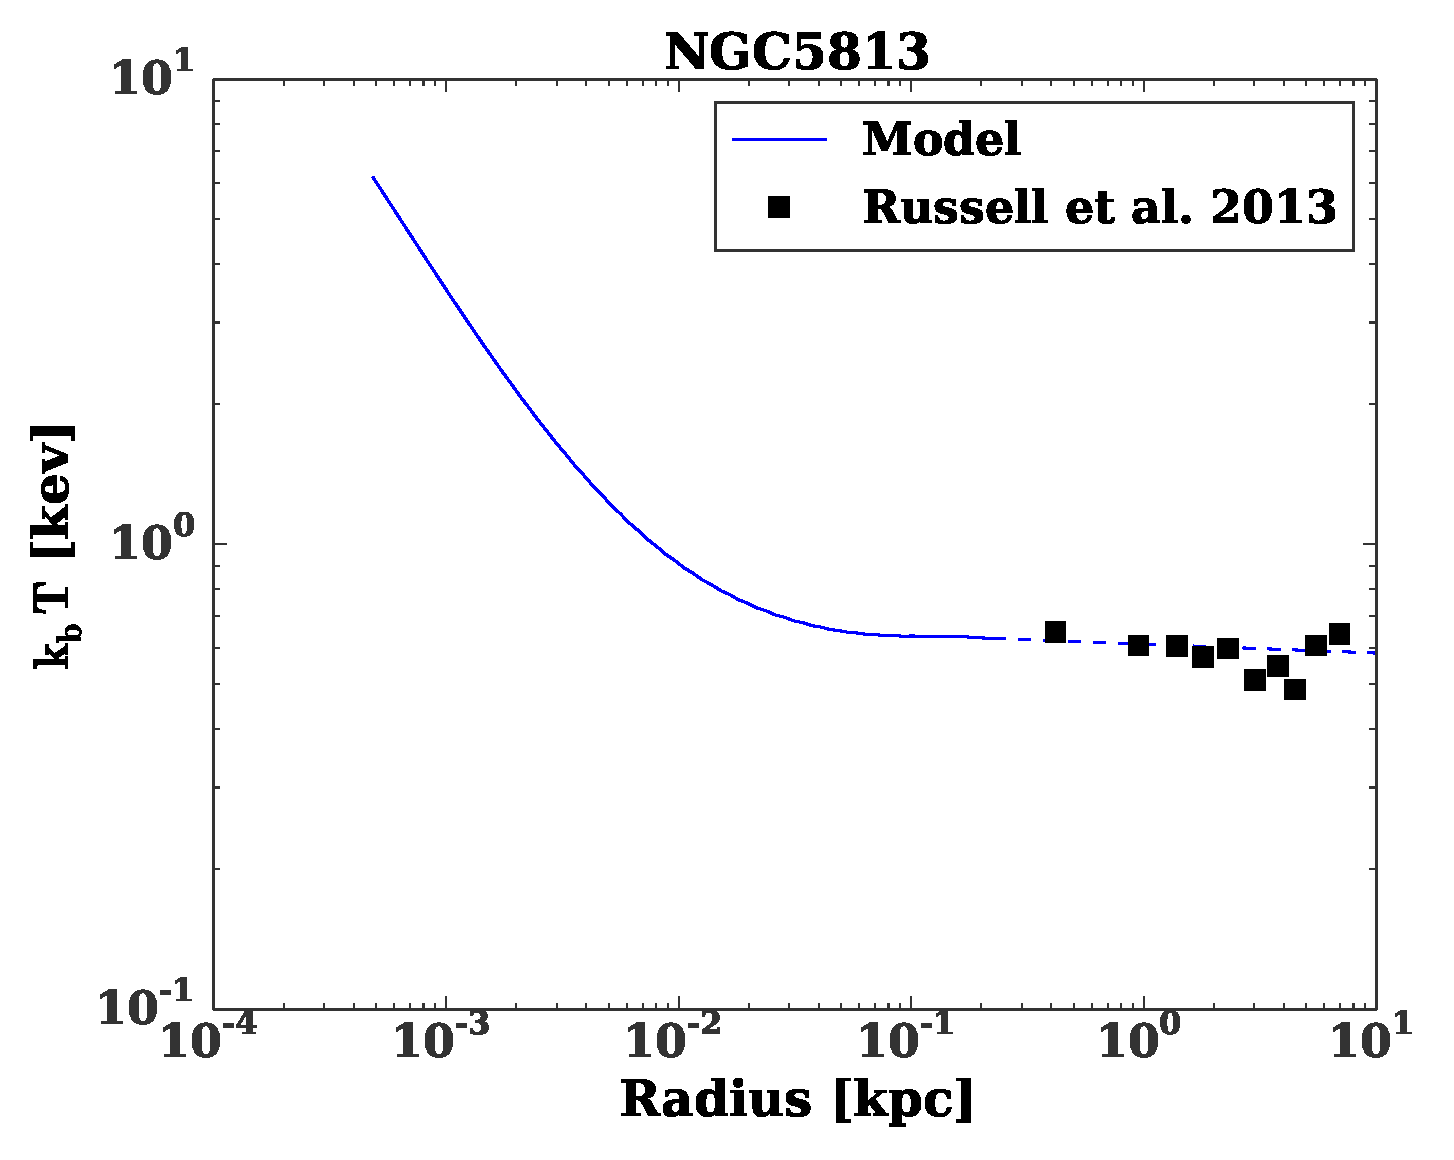
\includegraphics[width=\columnwidth]{NGC5813_T.eps}
%   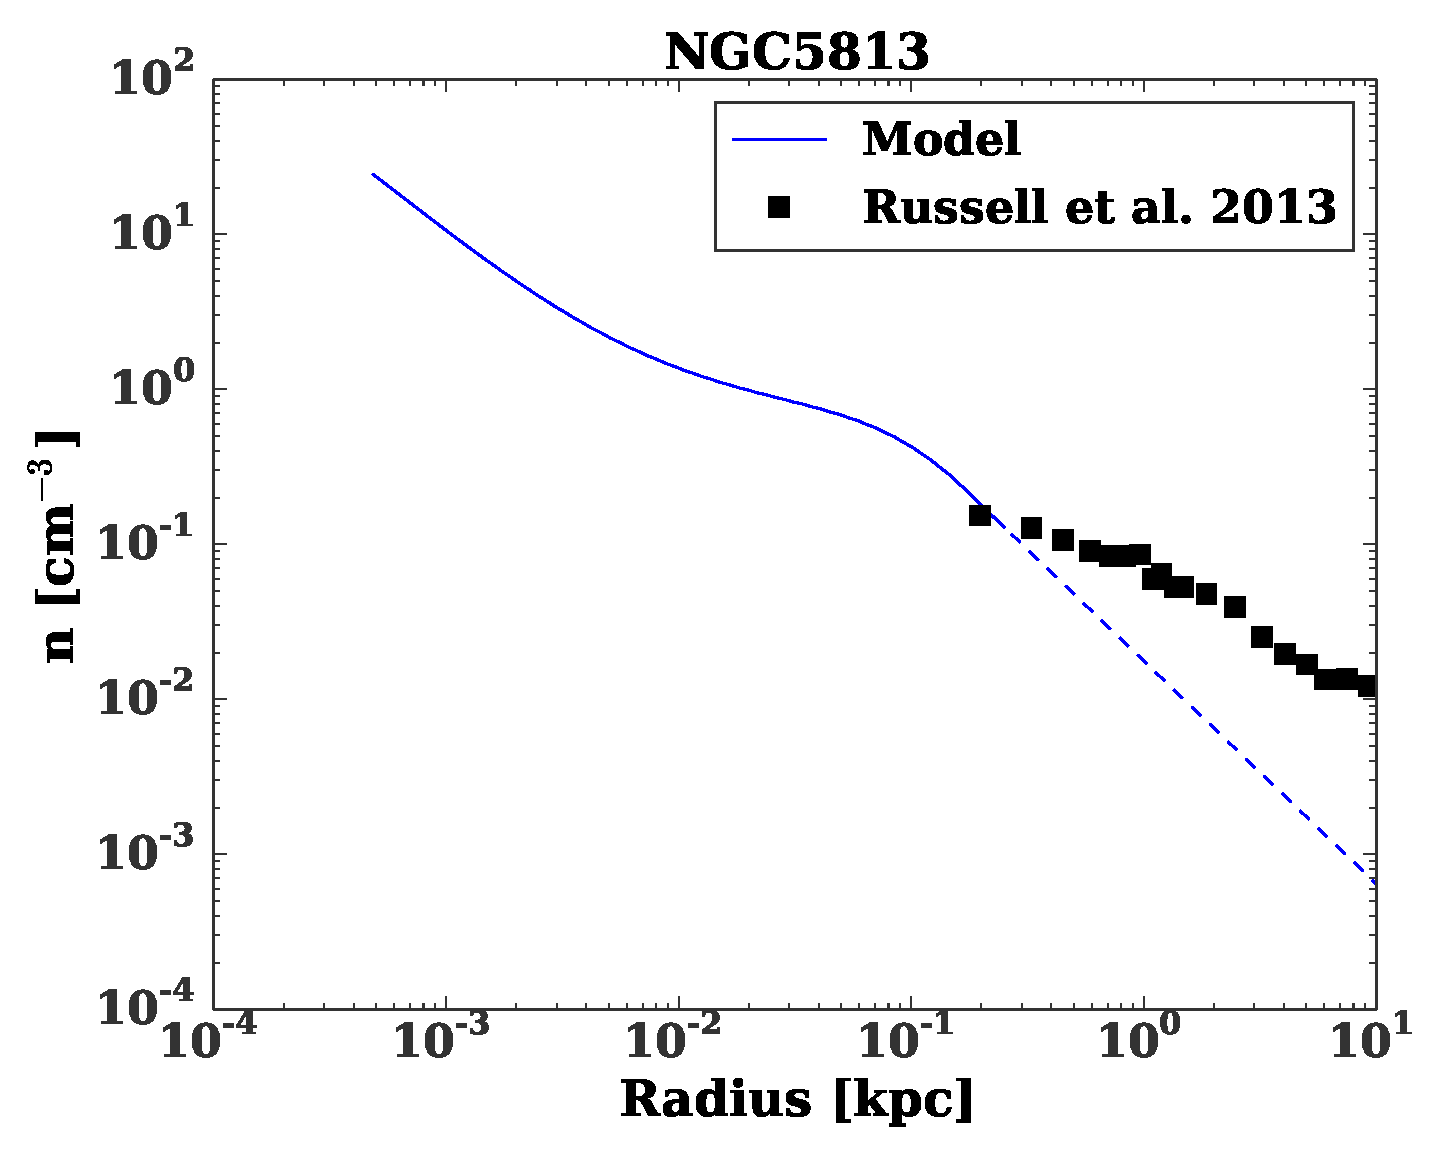
\includegraphics[width=\columnwidth]{NGC5813_rho.eps}
%   \caption{\label{fig:allen_compare} Comparison of the radial profiles
%     (blue lines) of electron number density $n_e$ and temperature $T$
%     to the measured values (black square) in \citet{AllenDunn+:2006a}
%     and \citet{ RussellMcNamara+:2013a}. The dashed blue lines are
%     power law extrapolations of our profiles. Note that in going from
%     $\rho$ to $n_e$ we our adopted value for the molecular weight $\mu=1$.}
%   %% AG in the future we will have to be carfeful of the mean molecular weight.
% \end{figure*}

% \subsubsection{Comparison with observed X-ray Luminosity-Mass
%   Relation}
% %Note currently I reverse-engineer the stellar mass from the black
% %hole mass inferred from M-sigma; however, it would be better to use
% %the tabulated black hole mass from the Mbh-Mbulge relation.
% Fig. 1 of \citealt{Miller+15} plots the observed
% relationship of unresolved x-ray luminosity versus galactic stellar
% mass for a sample of quiescent galaxies. We may construct a similar
% relationship with our own sample using the inferred accretion rates
% from our solutions.  To infer an x-ray luminosity for each solution,
% we scale our calculated $\Mdot c^2$ by a constant. We pick $5\times
% 10^{-7}$, which gives x-ray luminosities comparable to
% those in \citealt{Miller+15}. We also try an alternate
% prescription in which $L_x$ is quadratic in $\Mdot$. In particular, we
% take $L_x=2 \times 10^{-4} (\eddr) \Mdot c^2$. 

% We must make choose a $\vwO$ for each galaxy.  We select $\vwO$=200
% km/s if $\rs<\rIa$ for this solution, $\vwO$=500 km/s if $\rs>\rIa$
% for this solution, or exclude it.  At low $\Mbh$ we have $\vwO$=200
% km/s and at high $\Mbh$ we have $\vwO$=500 km/s.  Note that much of
% our sample is excluded in this Fig., since for $\vwO$=200 km/s we
% would have $\rs>\rIa$ and four $\vwO$=500 km/s we would have
% $\rs<\rIa$ (i.e. the relative locations of $\rs$ and $\rIa$ would be
% inconsistent with the assumed level of heating).

% %AG-power law may be closer to 1.4 & 1.8 than to 1.5 & 2.
% Our results are plotted in Fig.~\ref{fig:bh_xray}. In our model
% there is a steeper dependence $\Mbh$ on $M_{\rm gal}$ than in
% \citealt{Miller+15}. We find $L_x \propto M_{\rm gal}^{1.5}$ when
% $L_x \propto M_{\rm gal}^{2}$, whereas \citealt{Miller+15} finds
% that $L_x \propto M_{\rm gal}^{0.7-0.8}$. 

\section{Conclusions}
\label{sec:conclusions}

% Apologies: 
% \begin{itemize}
% \item{we assume that average star formation histories correspond to those experienced in the nuclear region.  }

% \item{ Do nuclear star clusters in other galaxies look like scaled
%     up/down versions of the one in our own galaxy? If so this would
%     imply a radial gradient in the average of the stellar population
%     which would imply a heating which would be dependent on radius.  }

% \end{itemize}


% However, \citet{McCourt+12} argue that even if cooling is exactly
% balanced by heating everywhere, there is still a local thermal
% instability that operates to turn hot gas into cold clouds.  However,
% this local instability only causes a significant local drop-out of
% mass from the hot medium (to low-T clouds), if the cooling timescale,
% \begin{align}
% \frac{\tcool}{\tff} &\equiv \frac{3\rho k T/2 \mu \mp}{\dot{q}_{\rm cool}} \approx \frac{9}{5} \left. \frac{q \vw^2/2}{\dot{q}_{\rm cool}}\right|_{\rs}
% \end{align} 
% is locally shorter than the approximately 10 times the free-fall
% timescale $t_{\rm ff}$, where the last equality is evaluated at the
% stagnation radius and makes use of equations~(\ref{eq:Tanalytic}) and
% (\ref{eq:rhors2}).  We thus see that the condition $\tilde{v}_{w} \gtrsim v_{\rm
%   crit}$ is also the condition for local instability, although the
% prefactor may be slightly different.


% If cooling becomes important in the flow ($\tilde{v}_{w} < v_{\rm CI}$), it may lead to thermal instabilities.  There are two kinds of ``instabilities", global and local.  The global instability is simply that, if cooling becomes very rapid, the gas loses thermal pressure and starts to inflow faster, i.e. the entire CNM accretes.  In
% practice this should could manifest as a large increase in the stagnation radius, due an effective {\it decrease} in the effective heating rate.  This global ``instability" is not a true instability insofar as the gas does not necessarily clump locally into low-T clouds.


We have calculated steady-state models for circumnuclear medium of
quiescent galaxies, assuming that gas is supplied entirely by stellar
wind mass loss and heated by shocked stellar winds, supernovae and
black hole feedback. We compute profiles for a range of different
black hole masses, heating rates, and stellar density profiles and use
these profiles to calculate an $\Mdot$ onto each galaxy's SMBH, and
get the scaling of $\Mdot$ with $\Mbh$. We may then compare our
results with observed trends of nuclear x-ray luminosity with galaxy
properties. Our main conclusions may be summarized as follows.

  \begin{enumerate}
  %Younger population=>higher accretion rate; generally higher eta and
  %lower vw except for very young stellar populations.
  \item We find that for $\Mbh\gsim 10^6 \Msun$ and $\Mbh\lsim 10^8
    \Msun$, $\eddr \propto \Mbh^{\alpha}$ with $\alpha\lsim
    0.5 \, (0.8)$ for core (cusp) galaxies, 
    following average star formation histories measured in
    cosmological simulations \citep{MosterNaab+:2013a}. This is in
    tension observations of nuclear X-ray luminosity which suggest
    that $\eddr$ increases towards smaller $\Mbh$
    \citep{Miller+15}. However, it is important to note that the
    inflow rate on large scales (which we calculate) may differ from
    the actual accretion rate as outflows could occur on small
    scales. The outflow rate would depend on the angular momentum of
    the infalling gas and thus the angular momentum of stars in the
    nucleus. The in turn would vary systematically with $\Mbh$.
  \item We expect within scatter in nuclear x-ray luminosities at
    fixed $\Mbh$ from (1) stochastic variation in star formation
    history from galaxy to galaxy (2) Variations in small scale outflow
    rates due to variations between galactic nuclear angular
    momenta. {\bf AG: some more explanation of why 1 might not show up
    in Pellegrini...}
    These variations alone could explain much of the 2-4 orders of
    magnitude of scatter of nuclear x-ray luminosity at fixed $\Mbh$ 
    in the samples of \citet{Miller+15} and \citet{Pellegrini:2010a}.
    
    It is also possible that many of the galaxies in the
    \citet{Miller+15} are accreting in a non-steady fashion and this
    scatter arises from cyclic variation in accretion rate. In fact it
    that a population of cyclically accreting with $\Mbh\gsim 10^{8}
    \Msun$ coexists with a population of smaller, steadily accreting
    black holes (e.g. the upper limits in \citet{Miller+15}).  This
    calls into question the use of simple extrapolations of power-law
    fits to the $L_{\rm X}(M_{\bullet}$) relationship to low $M_{\bullet}$
    to constrain the occupation fraction of black holes in low mass
    galaxies (\citealt{Miller+15}).
  \item Low mass AGN have growth times comparable to the Hubble time
    (\citet{Heckman+04}). We have shown that this would require accretion
    rates not consistent with steady-state thermally stable accretion
    of stellar wind material, and is driven by an external supply of gas.
  \item We compare the $\Mdot$ for each of our solution to the one
    calculated from the Bondi formula. We find that they agree to
    within a factor of order unity. This is because in our model the
    accretion rate is determined by the flow properties at the
    stagnation radius, $\rs$, which is within a factor of a few of the
    Bondi radius $\rb$. Thus, use of the Bondi formula is a
    good approximation.
    \end{enumerate}
   
    Overall we conclude that for values of $\Mbh\lsim 10^{8} \Msun$,
    the observed nuclear x-ray luminosities in quiescent, early type
    galaxies could be understood as coming from thermally stable
    steady-state accretion of stellar winds shed in the galactic
    nucleus.  However, we would like to draw attention to the
    following limitations of our model

    \begin{enumerate}
    \item Overall the accretion rate onto the cetral SMBH will be strongly
    tied to the properties of the stellar population (e.g. age) within
    the sphere of influence of the black hole. Thus, our model cannot
    say anything definitive about the mode accretion for indivudual
    galaxies which may have significant variations about our assumed
    average star formation histories.
    \item Also, the star formation history of bulges may (and probably
      does) systematically differ from the average star formation
      history for galaxies as a whole.
    \item Furthermore, there could be a radial gradient in the star
      formation history within a given bulge... 
    \end{enumerate}
  

  


  \clearpage
  \appendix
  \section{Analytic expression for the stagnation radius}
  \label{app:rs}
  
Here we derive an analytic expression for the steady-state stagnation radius $r_{\rm s}$.  The steady-state entropy equation (eq.~[\ref{eq:dsdt}]) can be manipulated to read
\begin{align}
T\dsdr=\frac{\Q}{\rho v} \label{eq:ss_entropy}
\end{align}
By definition, the velocity $v$ goes to zero at the stagnation radius.  In order to avoid the entropy derivate from diverging, the numerator of (\ref{eq:ss_entropy}) must also go to zero at $r_{\rm s}$, implying that
\begin{align}
 \frac{\gamma}{\gamma-1} \frac{p|_{\rs}}{\rho|_{\rs}}=\frac{\vw^{2}|_{\rs}}{2} \Rightarrow \frac{\kb T|_{\rs}}{\mu \mp}=\gammafi \frac{\vw^{2}|_{\rs}}{2} .
\label{eq:appTanalytic}
\end{align}
Combining (\ref{eq:ss_entropy}) with the first law of thermodynamics,
\begin{align}
T\dsdr =& \frac{1}{\gamma-1}\ddr{(p/\rho)}-\frac{p}{\rho^2}\ddr{\rho} = \\
& 
\frac{1}{\gamma-1}\left.\ddr{(p/\rho)}\right|_{\rs}+\frac{\densSlope}{\rs}  \frac{p|_{\rs}}{\rho|_{\rs}}=\left.\underbrace{\frac{\Q}{\rho  v}}_{A}\right|_{\rs}, 
% \label{eq:first_law}
\end{align}
where $\densSlope\equiv -\left.d\log(\rho)/d\log(r)\right|_{\rs}$.  The term on the right can be evaluated using L'Hopital's rule, yielding
%\begin{align}
 % &\lim_{r \rightarrow \rs} A=\frac{\lim_{r \rightarrow \rs}
  %  \frac{d}{dr}\left[q (r)\left(\ke -\gammaf
   %     \frac{p}{\rho}+\kew\right)\right]}{\lim_{r \rightarrow \rs}
    %\frac{d}{dr} \left(\rho v\right)}\\
  %&=\frac{ q'|_{\rs} \overbrace{\left.\left(\ke
   %     -\gammaf\frac{p}{\rho}+\kew\right)\right|_{\rs}}^0+ q|_{\rs}
    %\frac{d}{dr} \left[\left(\ke -\gammaf
     %   \frac{p}{\rho}+\kew\right)\right]_{\rs}}{\underbrace{\rho'|_{\rs}
      %v|_{\rs}}_0 +\underbrace{v'|_{\rs}\rho|_{\rs}}_{q|_{\rs}}}\\
\begin{align}
  \lim_{r \rightarrow \rs} A = \frac{d}{dr} \left[\left(\ke -\gammaf \frac{p}{\rho}+\kew\right)\right]_{\rs}
\end{align}
Now using the definition $\vw^2=\vwO^2+ G \Menc/r$, where
$\Menc=\Mbh+\Mstar$, and assuming $\Mstar \sim r^{2-\Gamma}$, we find that
\begin{align}
\lim_{r \rightarrow \rs} A=-\gammaf
\left.\ddr{(p/\rho)}\right|_{\rs}-\frac{G \Menc|_{\rs}}{2 \rs^2}+(2-\Gamma) \frac{G
  \Mstar|_{\rs}}{2 \rs^2}.
\end{align}
Substituting this expression back into equation (\ref{eq:first_law}) and using equation (\ref{eq:appTanalytic}) gives
\begin{align}
&\frac{\gamma+1}{\gamma-1}
\left.\ddr{(p/\rho)}\right|_{\rs}+ \frac{\gamma-1}{\gamma} \frac{\densSlope}{\rs} \vw|_{\rs}^{2} = (2-\Gamma) \frac{G
  \Mstar|_{\rs}}{2 \rs^2} -\frac{G \Menc|_{\rs}}{2 \rs^2}.  \label{eq:rs1}
\end{align}
A second equation results from evaluating the momentum equation (eq.~[\ref{eq:dvdt}]) at the stagnation point
\begin{align}
&\frac{1}{\rho}\dpdr=- \frac{G\Menc}{\rs^2} \Rightarrow
&\ddr{(p/\rho)}+\frac{p}{\rho}
\underbrace{\frac{d\log(\rho)}{dr}}_{-\densSlope/r} = -\frac{G \Menc}{\rs^2} \label{eq:HSE}
\end{align}
Finally, combining equations (\ref{eq:rs1}) and (\ref{eq:HSE}) gives 

\begin{align}
\rs=\frac{G \Mbh}{\densSlope \vw^{2}|_{\rs}}\left(\frac{9-\Gamma}{2}
  \frac{M_{\star}|_{\rs}}{\Mbh} +\frac{7}{2}\right),
\end{align}
where we have assumed $\gamma=5/3$.

In terms of just the additional wind heating parameter, $v_w$,

\begin{align}
\rs=\frac{G \Mbh}{\densSlope v_w^{2}|_{\rs}}\left[\left(\frac{9-\Gamma}{2} -\densSlope\right) \frac{\Mstar|_{\rs}}{\Mbh} +\frac{7}{2}-\densSlope\right].
\label{eq:rs2main}
\end{align}


Defining $\eta \equiv \vwO/\sigma_{\rm soi}$, this relationship can be
reparameterized as follows:
\begin{align}
  \frac{\rs}{\rsoi}=\frac{1}{2 \zeta^2 \densSlope}\left[
    \frac{\Mstar|_{\rs}}{\Mbh}\left(\frac{9-\Gamma}{2}-\densSlope\right)+\left(\frac{7}{2}-\densSlope\right)\right]
\end{align}

%{\bf AG: Note that I have taken sigmainf=2 G Mbh/rinf. Commented out
%equations have sigmainf=G Mbh/rinf}. 
For cusp galaxies ($\Gamma\simeq1$) we have $\Mstar|_{\rs}/\Mbh=x$, $A=4$, and $B=7/2$ for $\gamma = 5/3$, such that 
\begin{align}
\x=\frac{7-2\densSlope}{4\zeta^2 \densSlope+2\densSlope-8}
%\x=\frac{7-2\densSlope}{2\zeta^2 \densSlope+2\densSlope-8}
\end{align}
In the limit of zero wind heating $\eta \rightarrow 0$, no solution
for $r_{\rm s}$ exists unless the gas density profile at the
stagnation radius is steep, 3.5 $<\densSlope<$ 4.

For core galaxies ($\Gamma \simeq 0$) with $\Mstar/\Mbh=x^2$, A=9/2,
and B=7/2, the stagnation radius instead obeys a quadratic equation
\begin{align}
\x=\frac{\zeta^2 \densSlope \pm \sqrt{\zeta^4 \densSlope^2 - \left(\frac{9}{2}-\densSlope\right)
    \left(\frac{7}{2}-\densSlope\right)}}{\left(\frac{9}{2}-\densSlope\right)}
%\x=\frac{\zeta^2 \densSlope \pm \sqrt{\zeta^4 \densSlope^2 - 4 \left(\frac{9}{2}-\densSlope\right)
%\left(\frac{7}{2}-\densSlope\right)}}{2 \left(\frac{9}{2}-\densSlope\right)}
\label{eq:rstag}
\end{align}
In this case no solution exists in the zero heating limit ($\zeta
\rightarrow 0$) unless $3.5<\densSlope<4.5$.

When $\Mstar << \Mbh$ at the stagnation radius, the relationship
between $\rs$ and $\vw$ is greatly simplified.
\begin{align}
\rs=\frac{7}{2}\frac{G \Mbh}{\densSlope \vw^2},
\end{align}
where the pre-factor on the right-hand side corresponds to
$\gamma=5/3$ and $\Gamma=1$ or 0.  



%%% Local Variables:
%%% mode: latex
%%% TeX-master: "ms"
%%% Ennd:


  \section{Analytic expression for specific enthalpy of gas}
  {\bf AG: double check that what we are deriving here is actually
    specific enthalpy}
  \label{app:be}
  We derive an expression for the bernoulli parameter of the gas, $\ke
+\gammaf \frac{p}{\rho}+\Phi$, assuming that the stellar density
profile $\rhostar\sim r^{\delta}$ inside of the break radius $\rb$. 

Consider the steady state energy conservation equation. {\bf AG perhaps
  put a brief explanation of how this relates to the steady state
  entropy equation via laws of thermodynamics?.}

\begin{align}
\frac{1}{r^2} \frac{d}{dr} \left(r^2 \rho v \left(\frac{v^2}{2} + \Phi
    + \gammaf \frac{p}{\rho}\right) \right) = q \kew + q \Phi,
\label{eq:enCons}
\end{align}

Where $\vw^2=v_w^2+\sigma^2= v_w^2+\frac{3}{\Gamma+2}\frac{G
  \Mbh}{r}+\sigma_0^2$.

Now integrate both sides with respect from r to the stagnation radius 

\begin{align}
  r^2 \rho v \left(\ke+\Phi+\gammaf \frac{p}{\rho} \right)= \int_{\rs}^{r}
    r^2 \left(q \kew + q\Phi\right) dr
    \label{eq:enConsInt}
\end{align}

We know $f\equiv r^2 \rho v$ from the steady state mass conservation
equation. 

\begin{align}
 \frac{1}{r^2} \frac{d}{dr} \left(r^2 \rho v\right) = q 
\end{align}

Where q is the rate of the mass injection per volume, which is
proportional to the stellar density. Let $x=r/\rs$ and $q_o= q
(\rs)$. Then $q=q_o x^{-\delta}$. 

Then one obtains for the mass flux, $f=r^2 \rho v$,

\begin{align}
 f(x)=q_o \rs^3 \left[\frac{x^{3-\delta}-1}{3-\delta}\right].
 \label{eq:massFlux}
\end{align}

The gravitational potential $\Phi$ is given by

\begin{align}
\Phi&= -\frac{G \Menc}{r} - 4 \pi G \int_{r}^{\infty} \rhostar(r') r'
dr'.\nonumber\\
&\simeq -\frac{G \Menc}{r} -4 \pi G \int_{r}^{\rb} \rhostar(r') r' dr'
\label{eq:Phi}
\end{align}

Where in the scond line we have neglected the contribution of the
stars outside of the break radius, $\rb$, to the gravitational potential.

% Note our unconventional choice of gauge: the upper limit of the
% integral on the right hand side is $\rs$ whereas conventionally the
% upper limit is taken to be $\infty$. This means that our definition
% will not give $\Phi=0$ in the limit $r\rightarrow\infty$. However,
% our result for the enthalpy $\ke + \gammaf \frac{p}{\rho}$ will be
% gauge invariant. 

Using equations~\eqref{eq:enConsInt},~\eqref{eq:massFlux},
and~\eqref{eq:Phi}, we may obtain an expression for the Bernoulli
parameter of the gas, $\ke+\gammaf \frac{p}{\rho} +\Phi$ of the gas inside
of the break radius $\rb$.

\begin{align}
  &\frac{v^2}{2}+\gammaf \frac{p}{\rho} +\Phi = \nonumber\\
  &-U_o\left[\frac{\rs/\rb}{2-\delta}-\frac{x^{5-2\delta}-1}{x^{3-\delta}-1}\frac{3-\delta}{(5-2\delta)(2-\delta)}\right]\nonumber\\
  &+\frac{v_w^2}{2}+\frac{\sigma_0^2}{2}- \frac{G \Mbh}{r_s}
  \frac{1-2\delta}{2(\delta+1)} \frac{3-\delta}{2-\delta}\frac{x^{2-\delta}-1}{x^{3-\delta}-1}
  \nonumber\\
  &-\frac{G M_\star}{r_s}
  \frac{x^{5-2\delta}-1}{x^{3-\delta}-1}\frac{3-\delta}{5-2\delta},
\end{align}

where $U_o=4 \pi G \rhostar(\rs) \rs^2$.  We may rewrite this as 

\begin{multline}
  \frac{v^2}{2}+\gammaf \frac{p}{\rho}+\Phi
=\frac{G \Mbh}{\rs} 
\biggl[
  \frac{3}{2} \zeta^2 w^{\frac{1}{3 -\delta}}
  -\frac{(1-2\delta)(3-\delta)}{2(\delta+1)(2-\delta)}  \frac{x^{2  -\delta}-1}{x^{3-\delta}-1}\\
  -\frac{\rb}{\rsoi} w^{\frac{\delta-1}{3-\delta}} \frac{3 -\delta}{2 -\delta} 
  -w \frac{(2-\delta)(3-\delta)-(3-\delta)^{2}}{(5-2\delta)(2-\delta)} \frac{x^{5-2\delta}-1}{x^{3-\delta}-1}
\biggr].
\label{eq:enthAnal}
\end{multline}

Recall that $\rs$ the stagnation radius, $x\equiv r/\rs$, $\zeta=\sqrt{v_w^2+\sigma_0^2}/\sigma_0$, $w\equiv (\rs/\rsoi)^{3\delta}$, and
$\delta$ is the power law slope of the stellar density profile inside
of the break radius, $\rb$.

% For sufficiently large radii ($x$), the expression above always
% becomes negative, which means that a break in the stellar density
% profile is necessary in order to obtain an outflow.
 For a given $\rb/\rsoi$ there is a critical $\zeta$, $\zeta_{c}$, such
 that if $\zeta>\zeta_c$, an outflow will be possible from any
radius, since the Bernoulli parameter will be positive inside of the
break radius. On the other hand if $\zeta<\zeta_c$, then there is a
minimum value of $(\rs/\rsoi)_{\rm min}$. If we have had
$\rs/\rsoi<(\rs/\rsoi)_{\rm min}$, then the Bernoulli parameter would
become negative inside of $\rb$ and no outflow would be possible.

For cusp galaxies ($\Gamma$=0.8), $\zeta_c\simeq \sqrt 2$
($v_w\simeq\sigma_0$).  On the other hand for core galaxies
($\Gamma$=0.1) we find $\zeta_c\simeq (\rb/\rsoi)^{0.45}$, see the top
panel of Fig.~\ref{fig:zetaCrit}. For values of $\zeta<\zeta_c$, the
stagnation radius rapidly approaches the break radius as shown in the
bottom panel of Fig.~\ref{fig:zetaCrit}.
% We also find that for core galaxies for $\zeta<\zeta_c$, there is a minimum
% for $\rs/\rsoi$, $\left(\rs/\rsoi\right)_{\rm min}$--if $\rs/\rsoi$ were
% less than this value the gas enthalpy would become negative inside of
% the break radius which is clearly unphysical.  This may be roughly
% approximated using (see Fig.~\ref{fig:rbRinf})

% \begin{align}
% &\left.\frac{\rs}{\rsoi}\right|_{\rm min}=\frac{\rb}{\rsoi} \frac{\sqrt{\zeta_c-\zeta}}{\sqrt{\zeta_c-1}}\nonumber\\
% &\zeta_c\simeq \frac{\rb}{\rsoi}^{0.45}
% \label{eq:rsRinfCrit}
% \end{align}


\begin{figure}
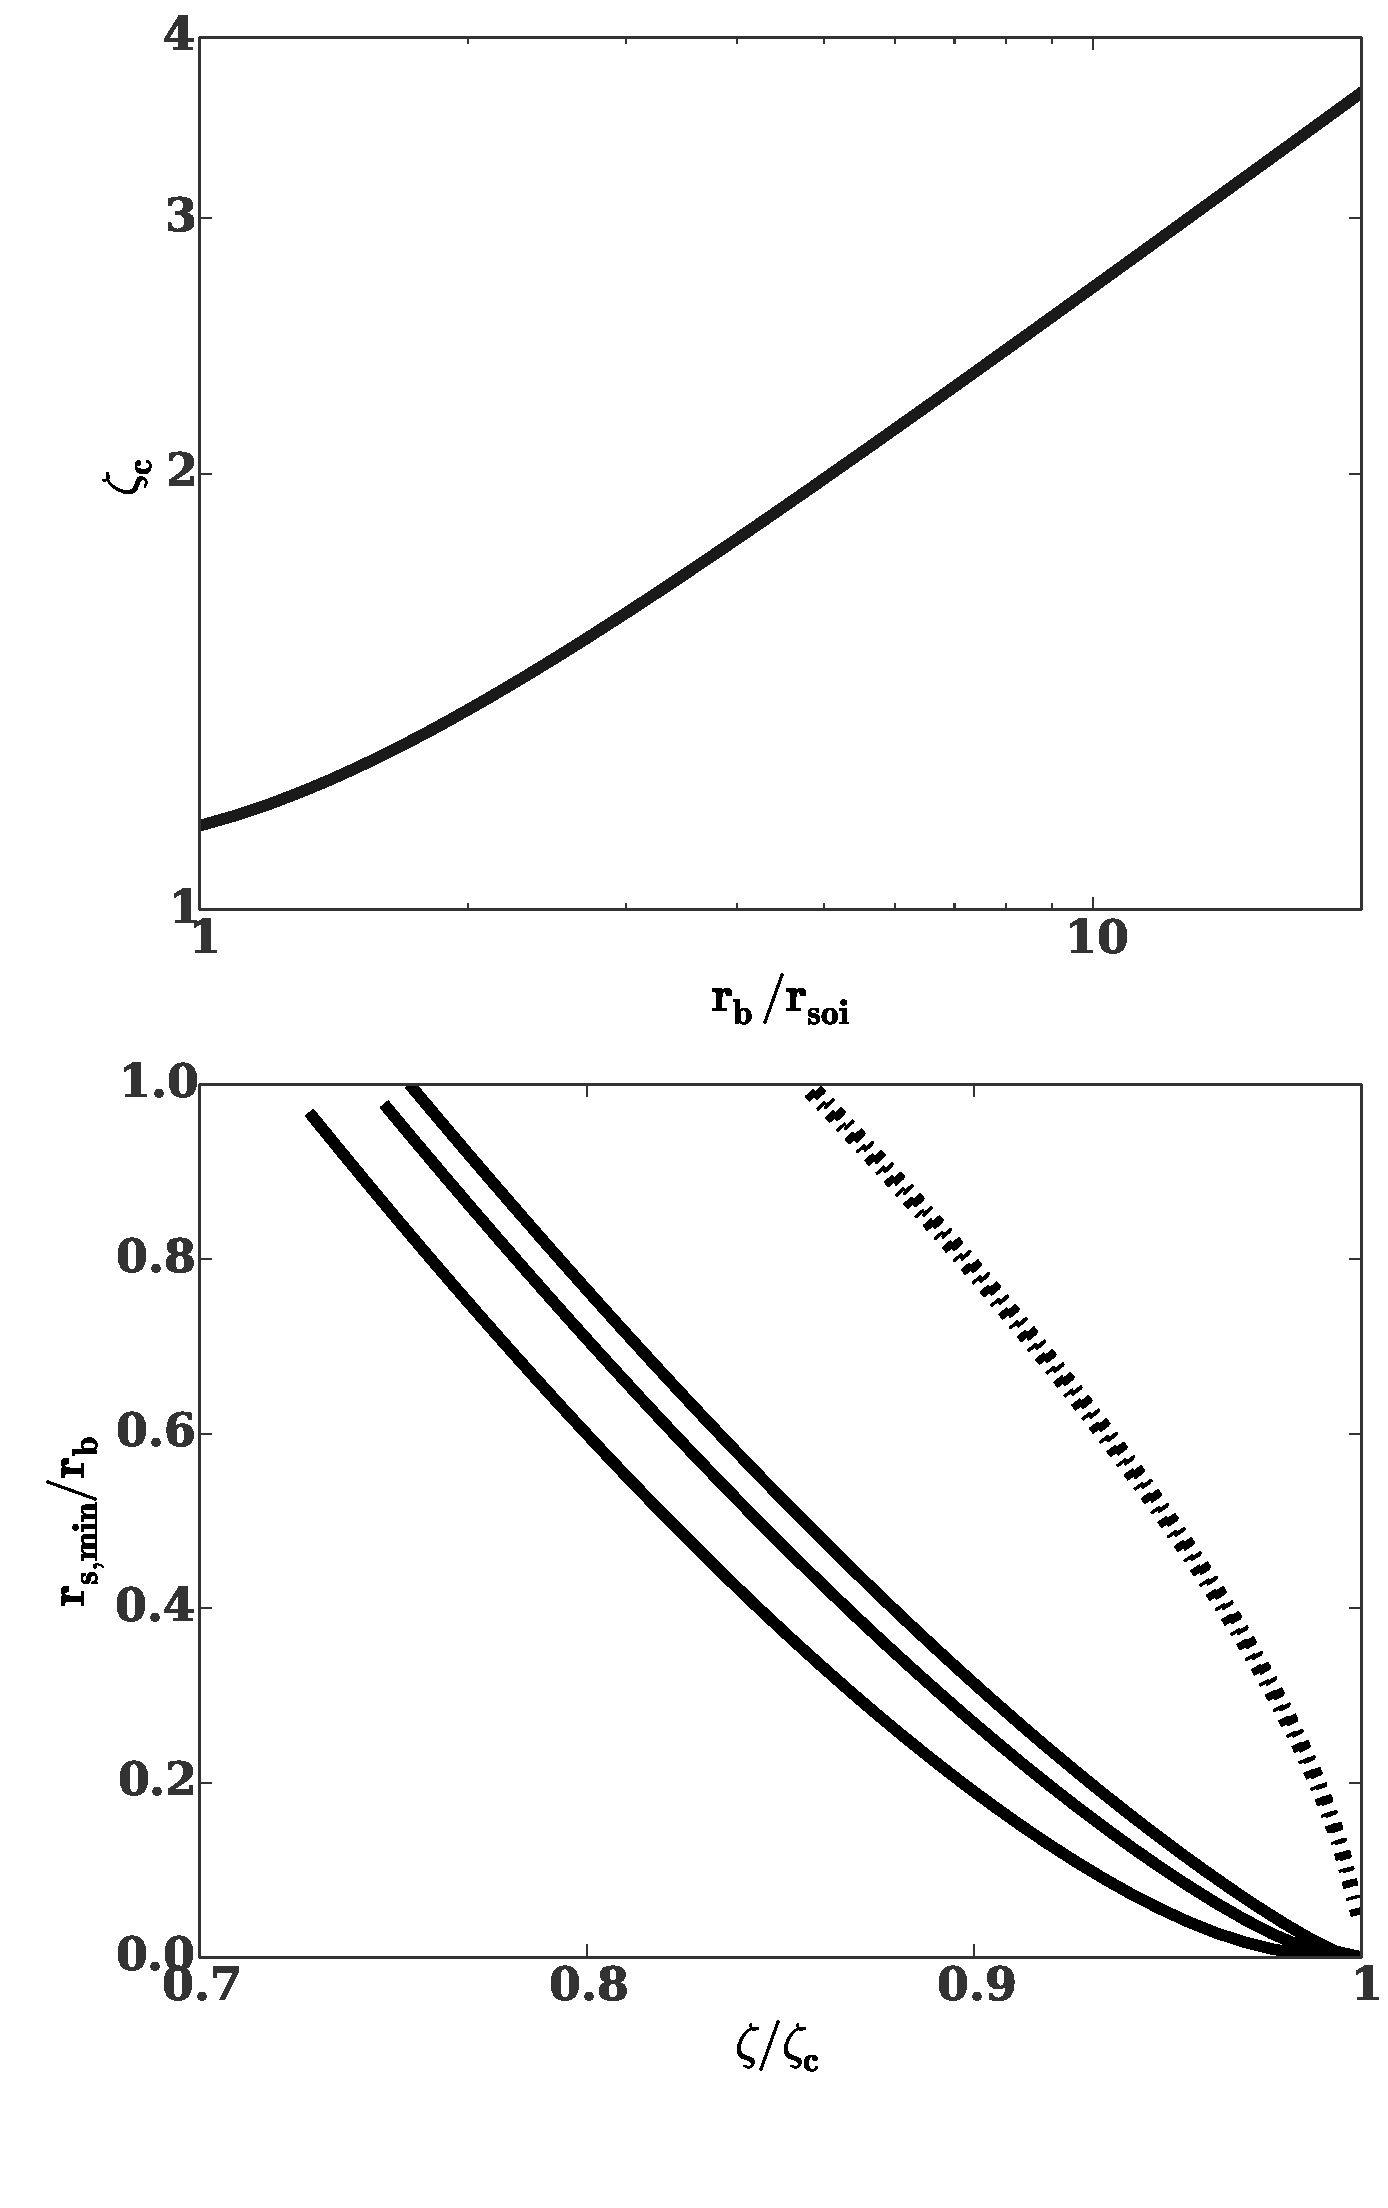
\includegraphics[width=\columnwidth]{zetaCrit.pdf}
\caption{\label{fig:zetaCrit} {\emph Top panel:} Critical
  $\zeta_c=\sqrt{v_w^2+\sigma_0^2}/\sigma_0$. If $\zeta<\zeta_c$ outflows are
  only possible if the ratio of the stagnation radius to the influence
  radius exceeds a minimum value. Plotted as a function of the ratio
  of the break radius to the influence radius ($\rb/\rsoi$) {\emph Bottom
    Panel:} Mininmum value for ratio of the stagnation radius to the
  influence radius, $\rs/\rsoi$ for core galaxies ($\Gamma=0.1$)
  derived by requiring enthalpy of the gas to remain positive out to
  the break radius $\rb$. This is calculated numerically from
  equation~\eqref{eq:enthAnal}. The x-intercept of each curve
  corresponds to the critical $\zeta_c$}
\end{figure}


%%% Local Variables: 
%%% mode: latex
%%% TeX-master: "ms"
%%% End: 


  \section{Analytic model for dependence of wind heating $\vwO^{\star}$ on stellar age}
\label{app:windheat}
% If we assume that a stellar population forms
% impulsively in the distant pass with IMF $\mu(m_*)$(with minimum mass
% $m_0$ and maximum mass $m_1$), then the surviving mass fraction at any
% future time $t$ is given by
% \begin{equation}
% f(t) =\frac{ \int_{m_0}^{m_{\rm T}(t)} m_* \mu(m_*) dm_* }{ \int_{m_0}^{m_1} m_* \mu(m_*) dm_* },
% \end{equation}
% where the main sequence turnoff mass is approximately
% \begin{equation}
% m_{\rm T}(t) \approx 2.5M_\odot~ \left( \frac{t}{10^9~{\rm yr}} \right)^{-0.4}.
% \end{equation}
% For a Salpeter IMF $\mu(m_*) \propto m_*^{-2.35}$ with $m_0=0.1M_\odot$ and $m_1=100M_\odot$,
% \begin{equation}
% f_{\rm Sal}(t) = 1.098 - 0.490 \left(\frac{t}{10^{10}~{\rm yr}} \right)^{0.14}
% \end{equation}
% {\bf NCS: we should probably use a Kroupa/Chabrier IMF, but this gets the ball rolling.}
% If we approximate post-main sequence evolution as instantaneous and define $\lambda(\Mstar)$ as the fractional mass lost during all stages of stellar evolution, then the mass loss rate density
% \begin{equation}
% q(t) = \frac{\rho_*}{\bar{m}_*} \lambda(m_{\rm T}(t)) m_{\rm T}(t) \frac{df}{dt},
% \end{equation}
% where the mean stellar mass $\bar{m}_* = \int_{m_0}^{m_{\rm T}(t)} \Mstar\mu(\Mstar)d\Mstar \approx 0.3 M_\odot$.  Further approximating $\lambda(\Mstar)=0.5$, and using the Salpeter IMF once more, gives
% \begin{equation}
% q(t) = \frac{\rho_*}{10^{10}~{\rm yr}} \times 0.11 \left(\frac{t}{10^{10}~{\rm yr}} \right)^{-1.26}.
% \end{equation}
% This is a specific, time-dependent definition of $\eta(t) (=0.11(t/t_{\rm h})^{-1.26})$; if we consider different star formation scenarios (for example, continuous star formation) or different IMFs, it will change.  Once these free parameters are specified, however, we can answer an important question: do young stellar populations increase or decrease the SMBH feeding rate $\dot{M}$?  Clearly, $\eta(t)$ is larger for young stellar populations, but these stars also have high wind velocities that diminish the stagnation radius.  Crudely approximating $v_{\rm w}=75~{\rm km~s}^{-1}$ for $m_{\rm T} < 10M_{\odot}$ and $v_{\rm w}=3000~{\rm km~s}^{-1}$ for $m_{\rm T} > 10M_{\odot}$ (motivated by the transition from dust-driven wind loss on the AGB to line-driven wind loss from Wolf-Rayet stars), we can employ the relation $\dot{M} \propto \eta(t) r_{\rm s}^{2-\Gamma}\propto \eta(t) v_{\rm w}^{-4+2\Gamma}$ (where $\rho_* \propto r^{-\Gamma}$) to determine the impact of stellar ``youth'' on SMBH feeding rates.
% {\bf AG:As I previously mentioned this discussion of the eta is not
%   quite correct...}
% \begin{figure}
% 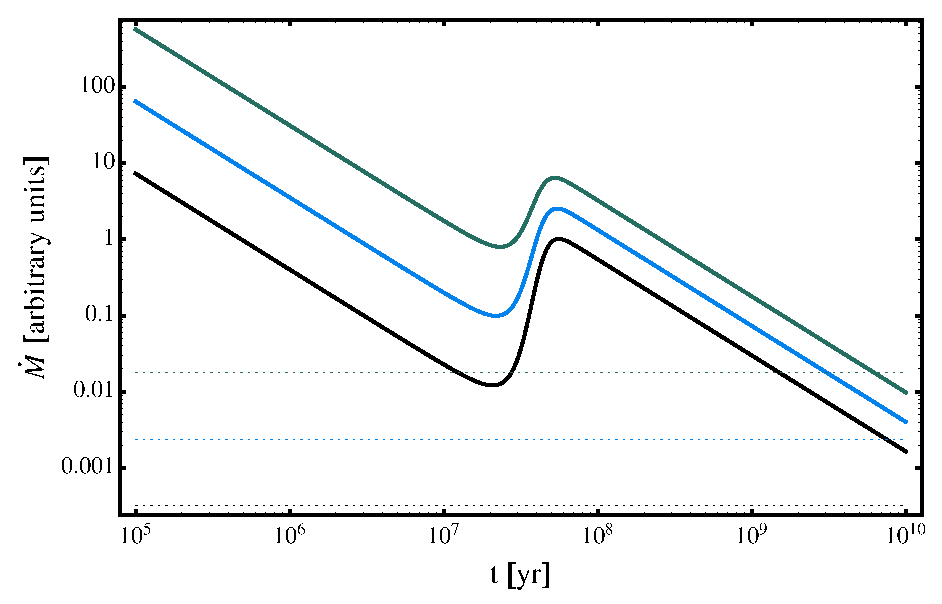
\includegraphics[width=\columnwidth]{NickPlot.eps}
% \caption{\label{NickPlot} SMBH feeding rates $\dot{M}=\eta(t) \times \Mstar(r_{\rm s})$, in arbitrary units.  The green, blue, and black curves are for galaxies with $\Gamma$ values of $0.1$, $0.5$, and $0.9$, respectively.  Solid curves represent impulsive-mode star formation, while dotted curves represent continuous-mode star formation. {\bf NCS: I think these old continuous curves are wrong, need to revise}}
% \end{figure}

% In Fig. \ref{NickPlot} we plot $\dot{M}$, in arbitrary units, as a
% function of time, for three different stellar density profiles $\Gamma
% = \{1.1, 1.5, 1.9\}$ (which are normalized to have the same mass at an
% influence radius $r _{\rm soi}=10~{\rm pc}$ around a $10^7M_\odot$
% SMBH).  We parametrize the wind velocity as
% \begin{equation} \frac{v_{\rm w}}{3000 ~\rm
% km~s^{-1}}=520-495\tanh\left( \frac{t-10^{7.5}~{\rm yr}}{10^{7}~{\rm
% yr}}\right). \label{NickV1}
% \end{equation} This counts Type II SNe heating as ``winds;'' if
% instead we are in the portion of parameter space where $r_{\rm II}$ is
% very large, then we use the alternate parametrization
% \begin{equation} \frac{v_{\rm w}}{3000 ~\rm
% km~s^{-1}}=520-495\tanh\left( \frac{t-10^{7}~{\rm yr}}{10^{6.5}~{\rm
% yr}}\right), \label{NickV2}
% \end{equation} which only allows short lived Wolf-Rayet stars to
% contribute to the high-heating mode.  The ``impulsive burst'' mode of
% star formation produces large ($\sim 10$) differences between the
% three $\dot{M}$ curves at early times, when $r_{\rm s}$ is small, but
% smaller ($\sim 3$) differences at late times, when $r_{\rm s}$ is
% large.  We also plot, as dotted curves, a simple model for the
% ``continuous'' mode of star formation, where mass loss is calculated
% as $\bar{\eta} = \int\eta(t)dt/t_{\rm h} \approx 4$ and an average
% energy injection in the wind is calculated as $\bar{v_{\rm
% w}^2}=\int\eta(t)v_{\rm w}^2(t)dt/\bar{\eta} \approx (800~{\rm
% km~s}^{-1})^2$.  Interestingly, the continuous mode of star formation
% produces small differences from late-time $\dot{M}$ seen in cusp
% galaxies with impulsive star formation; however, continuous mode star
% formation decreases late-time $\dot{M}$ by an order of magnitude
% relative to impulsive star formation in core galaxies.  {\bf NCS: I
% think this old discussion of MDot in the continuous limit is wrong,
% need to revise}

The energy and mass injection from stellar winds will be the sum ofthe
contributions from main sequence and post-main sequence (PMS) stars.
For an impulsively formed stellar population of age $t$, the mass
injection rate per unit stellar mass,$\dot{\bar{m}}(t)$, and  the energy
injection rate per unit stellar mass, $\dot{\bar{e}}(t)$,  will be given by

\begin{align} 
  \dot{\bar{m}}(t) &= \frac{\Delta M(t) \mu(M_{\rm TO}(t))
    \left|\dot{M}_{\rm TO}(t)\right| + f_{\rm MS} \int_{m_0}^{m_{\rm
        T}(t)}
    \dot{m}(\Mstar, t) \mu(\Mstar) {\rm d}\Mstar }{\bar{m}_*}\\
  \dot{\bar{e}}(t) &=\dot{e}_{\rm TO}(t)+ f_{\rm MS} \int_{m_0}^{m_{\rm T}(t)}
  \frac{\vw^2(\Mstar, t) \dot{m}(\Mstar, t) \mu(\Mstar) {\rm d}\Mstar}{\bar{m}_*}.
  \label{eq:edotImp}
\end{align} 

The first terms in each expression above correspond to the
contributions from PMS stars, while the second terms correspond to the
contributions from main sequence stars. The main sequence winds are a
small fraction of the mass, and they may be not be thermalized and
mixed with the rest of the injected gas. Thus, we include a
thermalization efficiency, $ 0\le f_{\rm MS}\le 1$, in
equation~\eqref{eq:edotImp}. Throughout this paper we set $f_{\rm
  MS}=1$. 

We assume a Salpeter IMF $\mu(\Mstar)\sim M^{-2.35}$, truncated at $0.1
\Msun$ on the low mass end and at $100 \Msun$ on the high mass
end. The corresponding mean stellar mass, $\bar{m}_*$ is 0.35 $\Msun$.

For the turnoff mass, $M_{\rm TO}$, we take the following fitting
formula 

\begin{align}
\log(M_{\rm TO})=0.24 + 0.068 x^2-0.34 x+4.76 e^{-4.58 x},
\end{align}

where $x=\log(t/10^9 {\rm years})$ and $M_{\rm TO}$ is in units
$\Msun$. This fit is designed to reproduce the results in 
Table 9 of \citet{MaederMeynet:1987a} and then asymptotes to the fit
for $M_{\rm TO}$ given in equation (9) of \citet{CiottiOstriker:2007a}
for intermediate and late times ($t \gsim 10^8$ years).

For $\Delta M(t)$ we use equation (10) from \citet{CiottiOstriker:2007a}

\begin{align}
\Delta M=
\begin{cases}
0.945 M_{\rm TO}-0.503 & M_{\rm TO} < 9 \Msun\\
 M_{\rm TO}-1.4 \Msun &  M_{\rm TO} \ge 9 \Msun
\end{cases}
\end{align}

To estimate the mass loss from main sequence stars
$\dot{m}(\Mstar, t)$,
we use equation 4 \citet{SchroderCuntz:2005a}\footnote{This
  prescription is a generalization of the Reimers' mass loss law. This
expression is derived assuming the stellar wind results from the
turbulent overflow of moaterial in the chromosphere or underneath it.} {\bf AG:
  unfortunately this is not really meant for MS stars...}

\begin{align}
  \dot{m}(\Mstar)=8 \times 10^{-14} \frac{L_* R_*}{\Mstar}
  \left(\frac{T_{\rm eff}}{\rm 4000 K}\right)^{3.5}
  \left(1+\frac{g_{\odot}}{4300 g_*}\right) \Msun \pyear,\
\end{align}

where  $R_*$, $L_*$, $T_{\rm eff}$ and $g_*$ are the stellar radius,
luminosity, effective and surface gravity respectively. $g_{\odot}$ is
the stellar surface gravity. To calculate $R_*$ and $L_*$ we use the
following scaling relations (taken from Kippenhann and Weygert Figures
22.2 and 22.3).

\begin{align}
L_*=
\begin{cases}
L_{\odot} (\Mstar/\Msun)^{3.2} & \Mstar > \Msun \\
L_{\odot} (\Mstar/\Msun)^{2.5} & \Mstar \le \Msun
\end{cases}
\end{align}

\begin{align}
r_*=
\begin{cases}
R_{\odot} (\Mstar/\Msun)^{0.57} & \Mstar > \Msun \\
R_{\odot} (\Mstar/\Msun)^{0.8} & \Mstar \le \Msun
\end{cases}
\end{align}


To get a handle on $\dot{e}_{\rm TO}(t)$, we use the results from
\citet{VossDiehl+:2009a} who use a population synthesis code to
simulate the mass and energy injection into the ISM from an OB
association. For the first $\sim 10$ Myr the energy injection will
come from energetic Wolf-Rayet star winds. The energy injection rate
per massive star ($\Mstar>8 \Msun$), $\dot{\mathcal{E}} (t)$, from
stellar winds is plotted in the top panel of their Figure 7 and is
well fit {\bf AG: A little more detail here...} by

\begin{align}
\dot{\mathcal{E}} (t)=
\begin{cases}
  1.3 \times 10^{36} {\rm ergs/s} & t<4 \times 10^6 {\rm years}\\
  1.3  \times 10^{36} {\rm ergs/s} \left(\frac{t}{4 \times  10^6}\right)^{-3.73} & t \ge 4 \times 10^6 {\rm years}.
\end{cases}
\label{eq:voss}
\end{align}

 $\dot{e}_{\rm TO}(t)$ is related to $\dot{\mathcal{E}}$  via 

\begin{align}
\dot{e}_{\rm TO}(t)=f_{8} \dot{\mathcal{E}} / \bar{m}_*,
\label{eq:eto}
\end{align}

where $f_{8}$ is the fraction of the stellar population with
$\Mstar>8 \Msun$. $f_8=2.6 \times 10^{-3}$ for our assumed Salpeter
IMF.  Equation~\eqref{eq:voss} and~\eqref{eq:eto} will be valid onlyfor $t
\lsim 10$ Myr. However, the turnoff contribution will become extremely
energetically subdominant at later times as far slower dust-driven
winds come to dominate the energy budget {\bf AG: Nick check--is the
  preceding sentence accurate}

We calculate the wind velocity for main sequence winds $v_w (\Mstar,
t)$ using...{\bf AG:Current just use the value for the sun~430 km/s
  replace with the real prescription we end up using.}

The effective wind velocity in the impulsive limit may then be written
as 

\begin{align}
\bar{v}_w(t)=2 \dot{\bar{e}}(t)/\dot{\bar{m}}(t)
\label{eq:vwImp}
\end{align}

We plot $\bar{v}_w$ in Figure~\ref{fig:vwImp}.

\begin{figure}
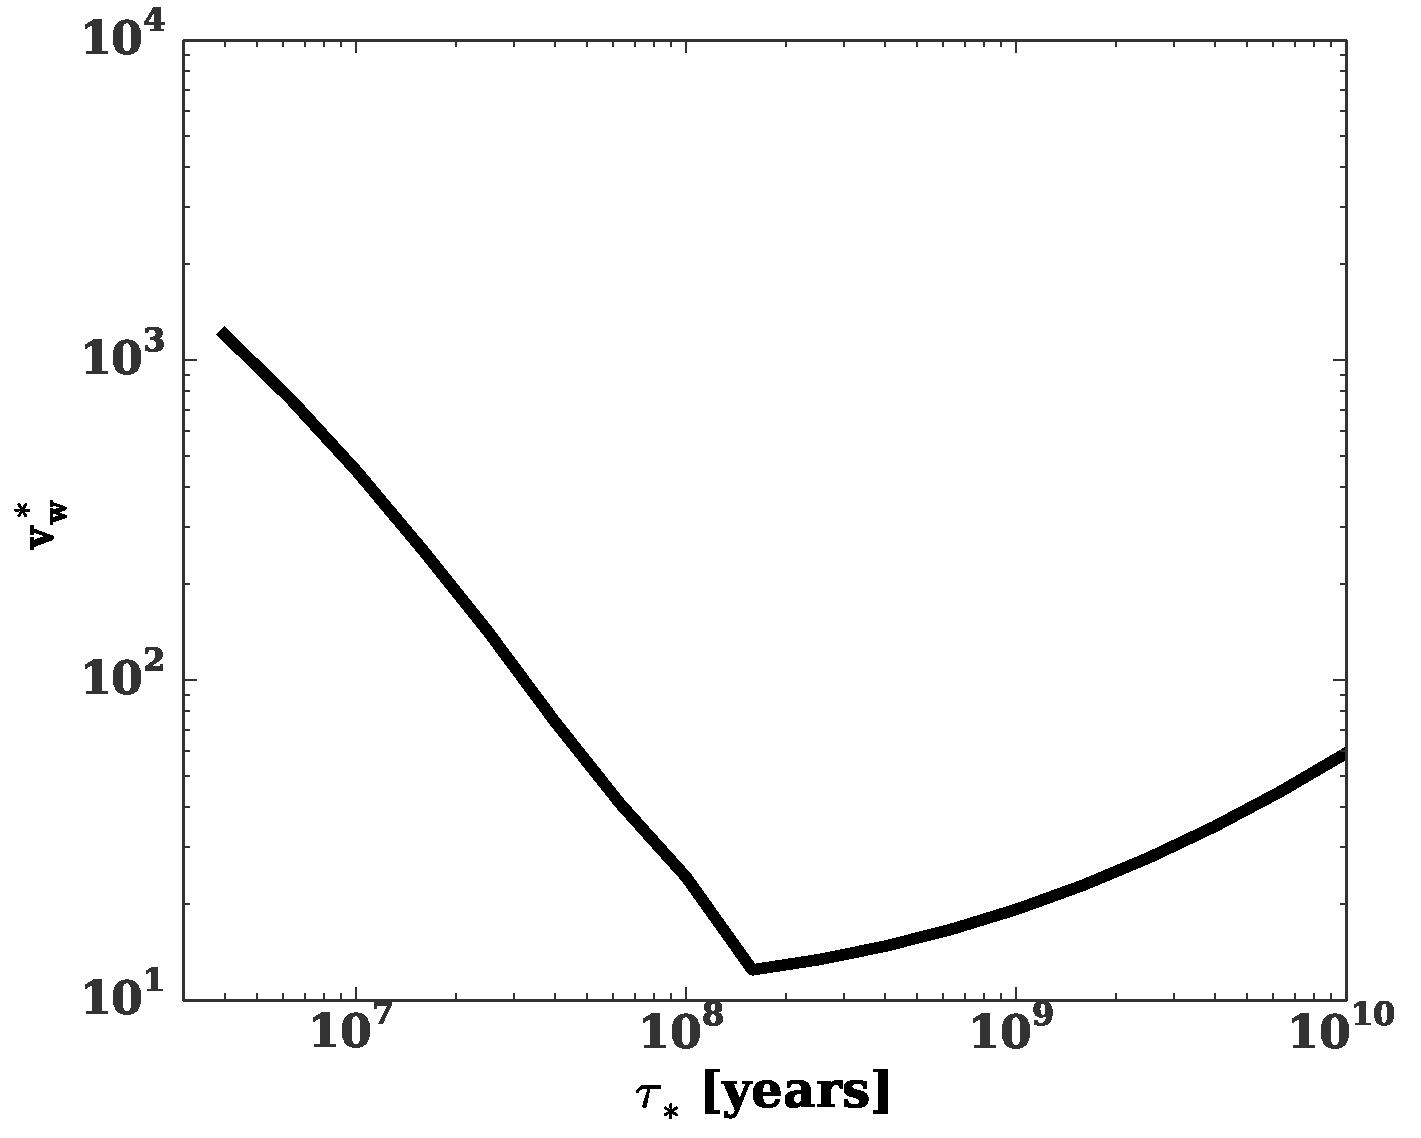
\includegraphics[width=\columnwidth]{vwImp.pdf}
\caption{\label{fig:vwImp} The effective $\vw$ from stellar winds from
  a stellar population formed in a starburst $t$ years ago.}
\end{figure}

We can then use these integrated quantities to determine the effective
$V_w$ for arbitrary star formation histories. For a stellar population
with star formation rate $S(t)$ 

\begin{align} 
  \dot{M}(t) &= \int_0^t S(t_1) \dot{\bar{m}}(t-t_1){\rm
      d}t_1\\
  \dot{E}(t) &= \int_0^t S(t_1) \dot{\bar{e}}(t-t_1){\rm
      d}t_1\\
  V_w^2(t) &=2 \dot{E}(t)/\dot{M}(t)
\end{align}

\begin{figure}
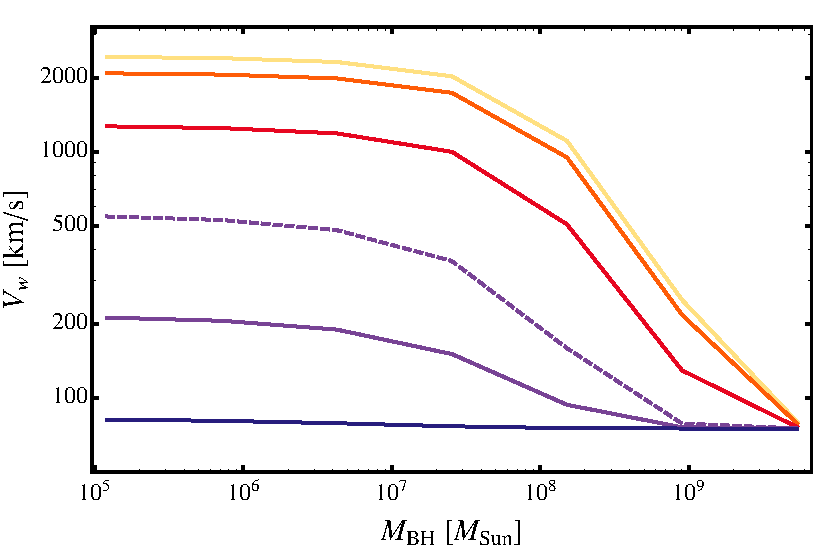
\includegraphics[width=\columnwidth]{vw.pdf}
\caption{\label{NickPlot2} Effective wind velocities $V_{\rm w}$ for
different $S(t)$.  The yellow and orange curves are the Moster SF
histories, with and without Type II SNe, respectively.  The red,
purple, and blue curves are Moster SFs convolved with a $\sin^2(t)$
function normalized to $10^7$, $10^8$, and $10^9$ yr fluctuations,
respectively.  These solid curves lack SN, but the dashed purple curve
possesses it.  Effective $V_{\rm w}$ is strongly diminished when the
variability timescale is greater than $\sim$ twice the duration of
high-velocity winds.}
\end{figure}

We show $V_{\rm W}$ for different star formation histories in
Fig. \ref{NickPlot2}.  In particular, we use Eqs. 17-20 from Moster et
al and the $M_{\rm BH}-M_{\rm halo}$ relation from Bandara et al {\bf
(NCS: add real refs)} to define $S(t)$ for particular galaxies.  It
seems that ``bumpy'' SF histories severely diminish $V_{\rm w}$ if the
timescale for SF variability is a factor of a few or more greater than
the duration of high-velocity winds (either 10 or 40 Myr).

%%% Local Variables: 
%%% mode: latex
%%% TeX-master: "ms"
%%% End: 


  \footnotesize{
    \bibliographystyle{mn2e}
    \bibliography{master}
  }
\end{document}
